% Options for packages loaded elsewhere
\PassOptionsToPackage{unicode}{hyperref}
\PassOptionsToPackage{hyphens}{url}
\PassOptionsToPackage{dvipsnames,svgnames,x11names}{xcolor}
%
\documentclass[
]{report}
\title{Ovarian Cancer Histotypes: Report of Statistical Findings}
\author{Derek Chiu}
\date{2021-12-10}

\usepackage{amsmath,amssymb}
\usepackage{lmodern}
\usepackage{iftex}
\ifPDFTeX
  \usepackage[T1]{fontenc}
  \usepackage[utf8]{inputenc}
  \usepackage{textcomp} % provide euro and other symbols
\else % if luatex or xetex
  \usepackage{unicode-math}
  \defaultfontfeatures{Scale=MatchLowercase}
  \defaultfontfeatures[\rmfamily]{Ligatures=TeX,Scale=1}
\fi
% Use upquote if available, for straight quotes in verbatim environments
\IfFileExists{upquote.sty}{\usepackage{upquote}}{}
\IfFileExists{microtype.sty}{% use microtype if available
  \usepackage[]{microtype}
  \UseMicrotypeSet[protrusion]{basicmath} % disable protrusion for tt fonts
}{}
\makeatletter
\@ifundefined{KOMAClassName}{% if non-KOMA class
  \IfFileExists{parskip.sty}{%
    \usepackage{parskip}
  }{% else
    \setlength{\parindent}{0pt}
    \setlength{\parskip}{6pt plus 2pt minus 1pt}}
}{% if KOMA class
  \KOMAoptions{parskip=half}}
\makeatother
\usepackage{xcolor}
\IfFileExists{xurl.sty}{\usepackage{xurl}}{} % add URL line breaks if available
\IfFileExists{bookmark.sty}{\usepackage{bookmark}}{\usepackage{hyperref}}
\hypersetup{
  pdftitle={Ovarian Cancer Histotypes: Report of Statistical Findings},
  pdfauthor={Derek Chiu},
  colorlinks=true,
  linkcolor={Maroon},
  filecolor={Maroon},
  citecolor={Blue},
  urlcolor={Blue},
  pdfcreator={LaTeX via pandoc}}
\urlstyle{same} % disable monospaced font for URLs
\usepackage[margin=1in]{geometry}
\usepackage{longtable,booktabs,array}
\usepackage{calc} % for calculating minipage widths
% Correct order of tables after \paragraph or \subparagraph
\usepackage{etoolbox}
\makeatletter
\patchcmd\longtable{\par}{\if@noskipsec\mbox{}\fi\par}{}{}
\makeatother
% Allow footnotes in longtable head/foot
\IfFileExists{footnotehyper.sty}{\usepackage{footnotehyper}}{\usepackage{footnote}}
\makesavenoteenv{longtable}
\usepackage{graphicx}
\makeatletter
\def\maxwidth{\ifdim\Gin@nat@width>\linewidth\linewidth\else\Gin@nat@width\fi}
\def\maxheight{\ifdim\Gin@nat@height>\textheight\textheight\else\Gin@nat@height\fi}
\makeatother
% Scale images if necessary, so that they will not overflow the page
% margins by default, and it is still possible to overwrite the defaults
% using explicit options in \includegraphics[width, height, ...]{}
\setkeys{Gin}{width=\maxwidth,height=\maxheight,keepaspectratio}
% Set default figure placement to htbp
\makeatletter
\def\fps@figure{htbp}
\makeatother
\setlength{\emergencystretch}{3em} % prevent overfull lines
\providecommand{\tightlist}{%
  \setlength{\itemsep}{0pt}\setlength{\parskip}{0pt}}
\setcounter{secnumdepth}{5}
\usepackage{titlesec, blindtext, color, float}

\titleformat{\chapter}[display]
  {\Huge\bfseries}
  {}
  {0pt}
  {\thechapter.\ }

\titleformat{name=\chapter,numberless}[display]
  {\Huge\bfseries}
  {}
  {0pt}
  {}

\titlespacing*{\chapter}{0pt}{0pt}{40pt}

\renewcommand{\bibname}{References}
\usepackage{booktabs}
\usepackage{longtable}
\usepackage{array}
\usepackage{multirow}
\usepackage{wrapfig}
\usepackage{float}
\usepackage{colortbl}
\usepackage{pdflscape}
\usepackage{tabu}
\usepackage{threeparttable}
\usepackage{threeparttablex}
\usepackage[normalem]{ulem}
\usepackage{makecell}
\usepackage{xcolor}
\ifLuaTeX
  \usepackage{selnolig}  % disable illegal ligatures
\fi
\usepackage[]{natbib}
\bibliographystyle{apalike}

\begin{document}
\maketitle

{
\hypersetup{linkcolor=}
\setcounter{tocdepth}{1}
\tableofcontents
}
\listoffigures
\listoftables
\hypertarget{preface}{%
\chapter*{Preface}\label{preface}}
\addcontentsline{toc}{chapter}{Preface}

This report of statistical findings describes the classification of ovarian cancer histotypes using data from NanoString CodeSets.

Marina Pavanello conducted the initial exploratory data analysis, Cathy Tang implemented class imbalance techniques, Derek Chiu conducted the normalization and statistical analysis, and Lauren Tindale and Aline Talhouk are the project leads.

\hypertarget{introduction}{%
\chapter{Introduction}\label{introduction}}

Ovarian cancer has five major histotypes: high-grade serous carcinoma (HGSC), low-grade serous carcinoma (LGSC), endometrioid carcinoma (ENOC), mucinous carcinoma (MUC), and clear cell carcinoma (CCOC). A common problem with classifying these histotypes is that there is a class imbalance issue. HGSC dominates the distribution, commonly accounting for 70\% of cases in many patient cohorts, while the other four histotypes are spread over the rest of the cases. Subsampling methods like up-sampling, down-sampling, and SMOTE can be used to mitigate this problem.

The supervised learning is performed under a consensus framework: we consider various classification algorithms and use evaluation metrics like accuracy, F1-score, Kappa, and G-mean to inform the decision of which methods to carry forward for prediction in confirmation and validation sets.

\hypertarget{methods}{%
\chapter{Methods}\label{methods}}

We use 5 classification algorithms and 4 subsampling methods across 500 repetitions in the supervised learning framework for the Training Set, CS1 and CS2. The pipeline was run using SLURM batch jobs submitted to a partition on a CentOS 7 server. Implementations of the techniques below were called from the \href{https://alinetalhouk.github.io/splendid/}{splendid} package.

\begin{itemize}
\item
  Classifiers:

  \begin{itemize}
  \tightlist
  \item
    Random Forest
  \item
    SVM
  \item
    Adaboost
  \item
    Multinomial Regression Model with Ridge Penalty
  \item
    Multinomial Regression Model with LASSO Penalty
  \end{itemize}
\item
  Subsampling:

  \begin{itemize}
  \tightlist
  \item
    None
  \item
    Down-sampling
  \item
    Up-sampling
  \item
    SMOTE
  \end{itemize}
\end{itemize}

\hypertarget{distributions}{%
\chapter{Distributions}\label{distributions}}

\hypertarget{full-data}{%
\section{Full Data}\label{full-data}}

The histotype distributions on the full data are shown below.

\begin{table}

\caption{\label{tab:dist-all-hist-gr}All CodeSet Histotype Groups}
\centering
\begin{tabular}[t]{l|r|r|r}
\hline
Histotype Group & CS1 & CS2 & CS3\\
\hline
HGSC & 126 & 655 & 1779\\
\hline
non-HGSC & 168 & 223 & 639\\
\hline
\end{tabular}
\end{table}

\begin{table}

\caption{\label{tab:dist-major-hist}All CodeSet Major Reviewed Histotypes}
\centering
\begin{tabular}[t]{l|r|r|r|r|r|r}
\hline
Reviewed Histotype & CS1 & CS2 & CS3 & CS1 \% & CS2 \% & CS3 \%\\
\hline
CCOC & 48 & 61 & 181 & 17.5 & 7.3 & 7.7\\
\hline
ENOC & 60 & 34 & 268 & 21.8 & 4.1 & 11.4\\
\hline
HGSC & 126 & 655 & 1779 & 45.8 & 78.6 & 75.8\\
\hline
LGSC & 21 & 21 & 42 & 7.6 & 2.5 & 1.8\\
\hline
MUC & 20 & 62 & 77 & 7.3 & 7.4 & 3.3\\
\hline
\end{tabular}
\end{table}

\begin{table}

\caption{\label{tab:dist-all}All CodeSet Reviewed Histotypes}
\centering
\begin{tabular}[t]{l|r|r|r}
\hline
Reviewed Histotype & CS1 & CS2 & CS3\\
\hline
CARCINOMA-NOS & 0 & 1 & 23\\
\hline
CCOC & 48 & 61 & 181\\
\hline
CTRL & 0 & 12 & 0\\
\hline
ENOC & 60 & 34 & 268\\
\hline
HGSC & 126 & 655 & 1779\\
\hline
LGSC & 21 & 21 & 42\\
\hline
MBOT & 0 & 20 & 3\\
\hline
MIXED (ENOC/CCOC) & 0 & 0 & 1\\
\hline
MIXED (ENOC/LGSC) & 0 & 0 & 1\\
\hline
MIXED (HGSC/CCOC) & 0 & 0 & 1\\
\hline
MMMT & 0 & 0 & 30\\
\hline
MUC & 20 & 62 & 77\\
\hline
Other (use when 6, 7, or 9 is not distinguished) or unknown if epithelial & 0 & 0 & 1\\
\hline
Other/Exclude & 0 & 0 & 8\\
\hline
SBOT & 19 & 12 & 2\\
\hline
serous LMP & 0 & 0 & 1\\
\hline
\end{tabular}
\end{table}

\begin{table}

\caption{\label{tab:dist-cs1}CS1 Histotypes}
\centering
\begin{tabular}[t]{l|l|r}
\hline
CodeSet & Reviewed Histotype & n\\
\hline
CS1 & CCOC & 48\\
\hline
CS1 & ENOC & 60\\
\hline
CS1 & HGSC & 126\\
\hline
CS1 & LGSC & 21\\
\hline
CS1 & MUC & 20\\
\hline
CS1 & SBOT & 19\\
\hline
\end{tabular}
\end{table}

\begin{table}

\caption{\label{tab:dist-cs2}CS2 Histotypes}
\centering
\begin{tabular}[t]{l|l|r}
\hline
CodeSet & Reviewed Histotype & n\\
\hline
CS2 & CARCINOMA-NOS & 1\\
\hline
CS2 & CCOC & 61\\
\hline
CS2 & CTRL & 12\\
\hline
CS2 & ENOC & 34\\
\hline
CS2 & HGSC & 655\\
\hline
CS2 & LGSC & 21\\
\hline
CS2 & MBOT & 20\\
\hline
CS2 & MUC & 62\\
\hline
CS2 & SBOT & 12\\
\hline
\end{tabular}
\end{table}

\begin{table}

\caption{\label{tab:dist-cs3}CS3 Histotypes}
\centering
\begin{tabular}[t]{l|l|r}
\hline
CodeSet & Reviewed Histotype & n\\
\hline
CS3 & CARCINOMA-NOS & 23\\
\hline
CS3 & CCOC & 181\\
\hline
CS3 & ENOC & 268\\
\hline
CS3 & HGSC & 1779\\
\hline
CS3 & LGSC & 42\\
\hline
CS3 & MBOT & 3\\
\hline
CS3 & MIXED (ENOC/CCOC) & 1\\
\hline
CS3 & MIXED (ENOC/LGSC) & 1\\
\hline
CS3 & MIXED (HGSC/CCOC) & 1\\
\hline
CS3 & MMMT & 30\\
\hline
CS3 & MUC & 77\\
\hline
CS3 & Other (use when 6, 7, or 9 is not distinguished) or unknown if epithelial & 1\\
\hline
CS3 & Other/Exclude & 8\\
\hline
CS3 & SBOT & 2\\
\hline
CS3 & serous LMP & 1\\
\hline
\end{tabular}
\end{table}

\begin{table}

\caption{\label{tab:dist-common}Common Summary ID CodeSet Histotypes}
\centering
\begin{tabular}[t]{l|r|r|r}
\hline
Reviewed Histotype & CS1 & CS2 & CS3\\
\hline
CCOC & 3 & 4 & 9\\
\hline
ENOC & 4 & 4 & 9\\
\hline
HGSC & 59 & 62 & 95\\
\hline
LGSC & 7 & 5 & 8\\
\hline
MUC & 7 & 5 & 11\\
\hline
\end{tabular}
\end{table}

\hypertarget{training-set}{%
\section{Training Set}\label{training-set}}

The training set distributions for CS1 and CS2 are shown below.

\begin{table}

\caption{\label{tab:training-dist-cs1}CS1 Training Set Histotypes}
\centering
\begin{tabular}[t]{l|r|l}
\hline
Histotype & n & \%\\
\hline
CCC & 57 & 18.8\%\\
\hline
ENOCa & 59 & 19.4\%\\
\hline
HGSC & 156 & 51.3\%\\
\hline
LGSC & 16 & 5.3\%\\
\hline
MUC & 16 & 5.3\%\\
\hline
\end{tabular}
\end{table}

\begin{table}

\caption{\label{tab:training-dist-cs2}CS2 Training Set Histotypes}
\centering
\begin{tabular}[t]{l|r|l}
\hline
Histotype & n & \%\\
\hline
CCOC & 68 & 7.2\%\\
\hline
ENOC & 30 & 3.2\%\\
\hline
HGSC & 757 & 80.1\%\\
\hline
LGSC & 29 & 3.1\%\\
\hline
MUC & 61 & 6.5\%\\
\hline
\end{tabular}
\end{table}

\hypertarget{common-samples}{%
\section{Common Samples}\label{common-samples}}

\begin{table}

\caption{\label{tab:common-dist-all}All Common Samples Histotype Distribution}
\centering
\begin{tabular}[t]{l|r|r|r}
\hline
revHist & CS1 & CS2 & CS3\\
\hline
CCOC & 3 & 4 & 3\\
\hline
ENOC & 4 & 4 & 3\\
\hline
HGSC & 57 & 60 & 73\\
\hline
LGSC & 7 & 5 & 4\\
\hline
MUC & 7 & 5 & 5\\
\hline
\end{tabular}
\end{table}

\begin{table}

\caption{\label{tab:common-dist-distinct}Distinct Common Samples Histotype Distribution}
\centering
\begin{tabular}[t]{l|r|r|r}
\hline
revHist & CS1 & CS2 & CS3\\
\hline
CCOC & 3 & 3 & 3\\
\hline
ENOC & 3 & 3 & 3\\
\hline
HGSC & 55 & 55 & 55\\
\hline
LGSC & 4 & 4 & 4\\
\hline
MUC & 5 & 5 & 5\\
\hline
\end{tabular}
\end{table}

\begin{table}

\caption{\label{tab:common-cs2-cs3-dist-distinct}Distinct Common CS2 and CS3 Samples Histotype Distribution}
\centering
\begin{tabular}[t]{l|r|r}
\hline
revHist & CS2 & CS3\\
\hline
CCOC & 3 & 3\\
\hline
ENOC & 3 & 3\\
\hline
HGSC & 71 & 71\\
\hline
LGSC & 4 & 4\\
\hline
MUC & 5 & 5\\
\hline
\end{tabular}
\end{table}

\begin{table}

\caption{\label{tab:common-dist-sites}Common Samples Across Sites Histotype Distribution}
\centering
\begin{tabular}[t]{l|r|r|r}
\hline
revHist & AOC & USC & Vancouver\\
\hline
CCOC & 3 & 3 & 3\\
\hline
ENOC & 3 & 3 & 3\\
\hline
HGSC & 13 & 13 & 27\\
\hline
LGSC & 2 & 2 & 2\\
\hline
MUC & 3 & 3 & 3\\
\hline
\end{tabular}
\end{table}

\begin{table}

\caption{\label{tab:common-dist-sites-distinct}Distinct Common Samples Across Sites Histotype Distribution}
\centering
\begin{tabular}[t]{l|r|r|r}
\hline
revHist & AOC & USC & Vancouver\\
\hline
CCOC & 3 & 3 & 3\\
\hline
ENOC & 3 & 3 & 3\\
\hline
HGSC & 13 & 13 & 13\\
\hline
LGSC & 2 & 2 & 2\\
\hline
MUC & 3 & 3 & 3\\
\hline
\end{tabular}
\end{table}

\begin{table}

\caption{\label{tab:cs345-overlap}CS3/CS4/CS5 Common Samples Histotype Distribution}
\centering
\begin{tabular}[t]{l|r|r|r}
\hline
revHist & CS3 & CS4 & CS5\\
\hline
HGSC & 46 & 46 & 46\\
\hline
NA & 26 & 26 & 26\\
\hline
\end{tabular}
\end{table}

\begin{table}

\caption{\label{tab:cs345-pools}CS3/CS4/CS5 Pools Distribution}
\centering
\begin{tabular}[t]{l|r|r|r}
\hline
Pool & CS3 & CS4 & CS5\\
\hline
Pool1 & 12 & 5 & 4\\
\hline
Pool2 & 5 & 5 & 4\\
\hline
Pool3 & 5 & 5 & 4\\
\hline
Pool4 & NA & 2 & 1\\
\hline
Pool5 & NA & 2 & 1\\
\hline
Pool6 & NA & 2 & 0\\
\hline
Pool7 & NA & 2 & 1\\
\hline
Pool8 & NA & 2 & 1\\
\hline
Pool9 & NA & 2 & 1\\
\hline
Pool10 & NA & 2 & 1\\
\hline
Pool11 & NA & 2 & 1\\
\hline
\end{tabular}
\end{table}

\hypertarget{histotypes-in-classifier-data}{%
\section{Histotypes in Classifier Data}\label{histotypes-in-classifier-data}}

\begin{table}

\caption{\label{tab:train-hist-codeset}Full Training Set Histotype Distribution by CodeSet}
\centering
\begin{tabular}[t]{l|l|l|l|l|l}
\hline
Variable & Levels & CS1 & CS2 & CS3 & Total\\
\hline
Histotype & HGSC & 122 (49\%) & 629 (80\%) & 476 (94\%) & 1227 (79\%)\\
\hline
 & CCOC & 44 (18\%) & 54 (7\%) & 8 (2\%) & 106 (7\%)\\
\hline
 & ENOC & 55 (22\%) & 28 (4\%) & 8 (2\%) & 91 (6\%)\\
\hline
 & MUC & 16 (6\%) & 59 (7\%) & 9 (2\%) & 84 (5\%)\\
\hline
 & LGSC & 14 (6\%) & 19 (2\%) & 6 (1\%) & 39 (3\%)\\
\hline
Total & N (\%) & 251 (16\%) & 789 (51\%) & 507 (33\%) & 1547 (100\%)\\
\hline
\end{tabular}
\end{table}

\begin{table}

\caption{\label{tab:hist-codeset-dataset}Histotype Distribution by CodeSet/Datasets}
\centering
\begin{tabular}[t]{l|l|l|l|l|l}
\hline
Variable & Levels & CS1 All & CS2 All & Confirmation & Validation\\
\hline
Histotype & HGSC & 125 (47\%) & 654 (79\%) & 423 (66\%) & 781 (74\%)\\
\hline
 & CCOC & 47 (18\%) & 60 (7\%) & 75 (12\%) & 86 (8\%)\\
\hline
 & ENOC & 58 (22\%) & 32 (4\%) & 106 (16\%) & 140 (13\%)\\
\hline
 & MUC & 19 (7\%) & 61 (7\%) & 27 (4\%) & 34 (3\%)\\
\hline
 & LGSC & 19 (7\%) & 20 (2\%) & 13 (2\%) & 20 (2\%)\\
\hline
Total & N (\%) & 268 (10\%) & 827 (30\%) & 644 (23\%) & 1061 (38\%)\\
\hline
\end{tabular}
\end{table}

\hypertarget{results}{%
\chapter{Results}\label{results}}

We show internal validation summaries for the combined classifier training set, as well as the CS1 and CS2 sets with duplicates included. The F1-scores, kappa, and G-mean are the measures of interest. Algorithms are sorted by descending value based on the overallaccuracy of the training set. The point ranges show the median, 5th and 95th percentiles, coloured by subsampling methods.

\hypertarget{training-set-1}{%
\section{Training Set}\label{training-set-1}}

\hypertarget{accuracy}{%
\subsection{Accuracy}\label{accuracy}}

\begin{figure}[H]

{\centering 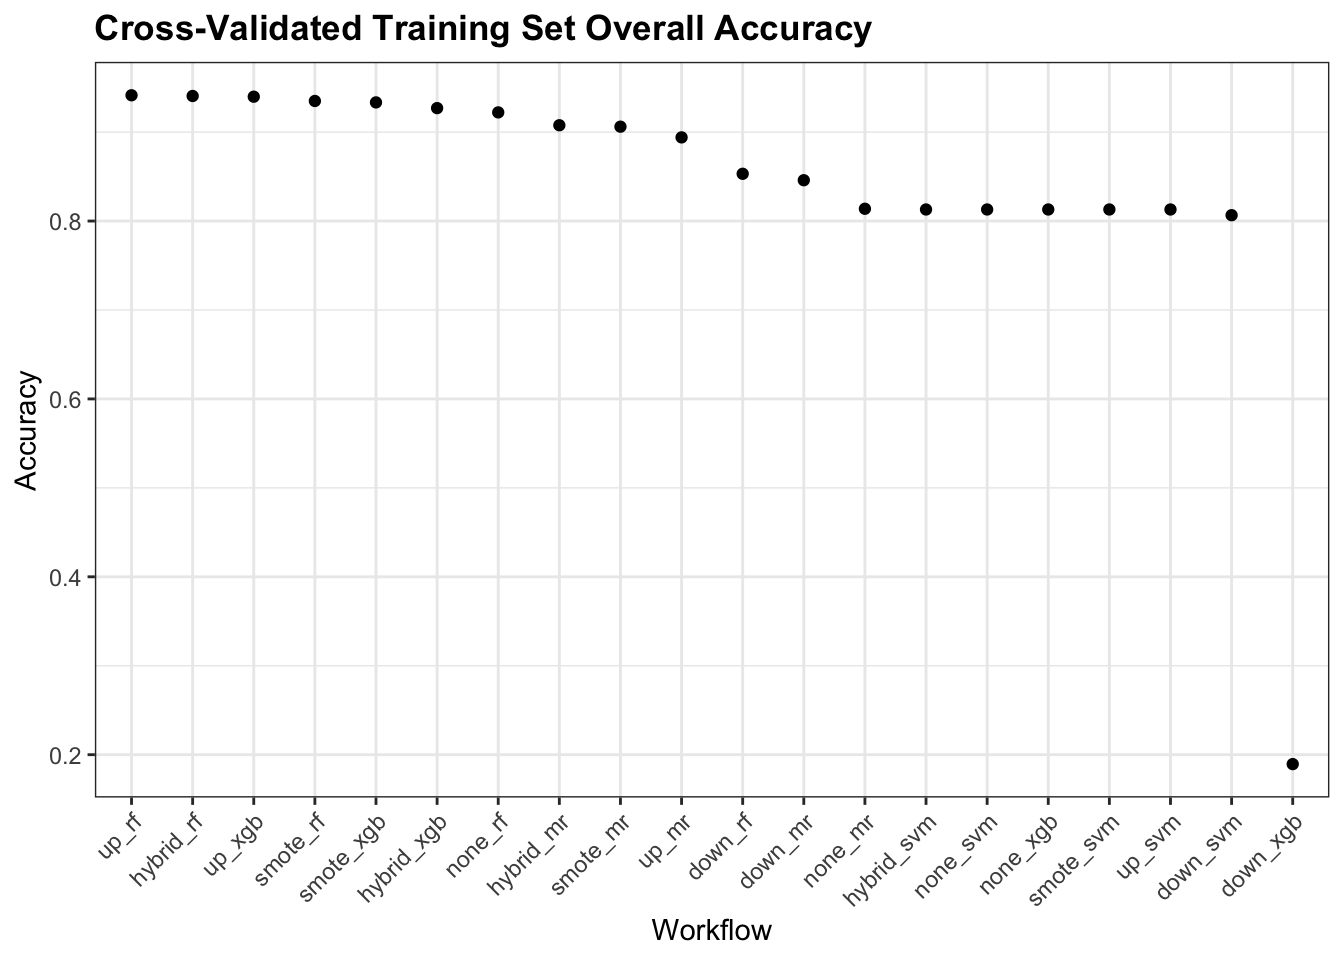
\includegraphics{OV_Histotypes_RSF_files/figure-latex/train-accuracy-1} 

}

\caption{Training Set Accuracy}\label{fig:train-accuracy}
\end{figure}

\begin{table}

\caption{\label{tab:train-accuracy-table}Training Set Accuracy by Algorithm and Subsampling Method}
\centering
\begin{tabular}[t]{l|l|l|l|l|l}
\hline
sampling & rf & svm & adaboost & mlr\_ridge & mlr\_lasso\\
\hline
none & 0.932 & 0.938 & 0.921 & 0.931 & 0.93\\
\hline
up & 0.937 & 0.936 & \textbf{0.94} & 0.893 & 0.903\\
\hline
down & 0.871 & 0.868 & 0.865 & 0.853 & 0.834\\
\hline
smote & 0.939 & 0.933 & 0.929 & 0.908 & 0.907\\
\hline
\end{tabular}
\end{table}

\begin{figure}[H]

{\centering 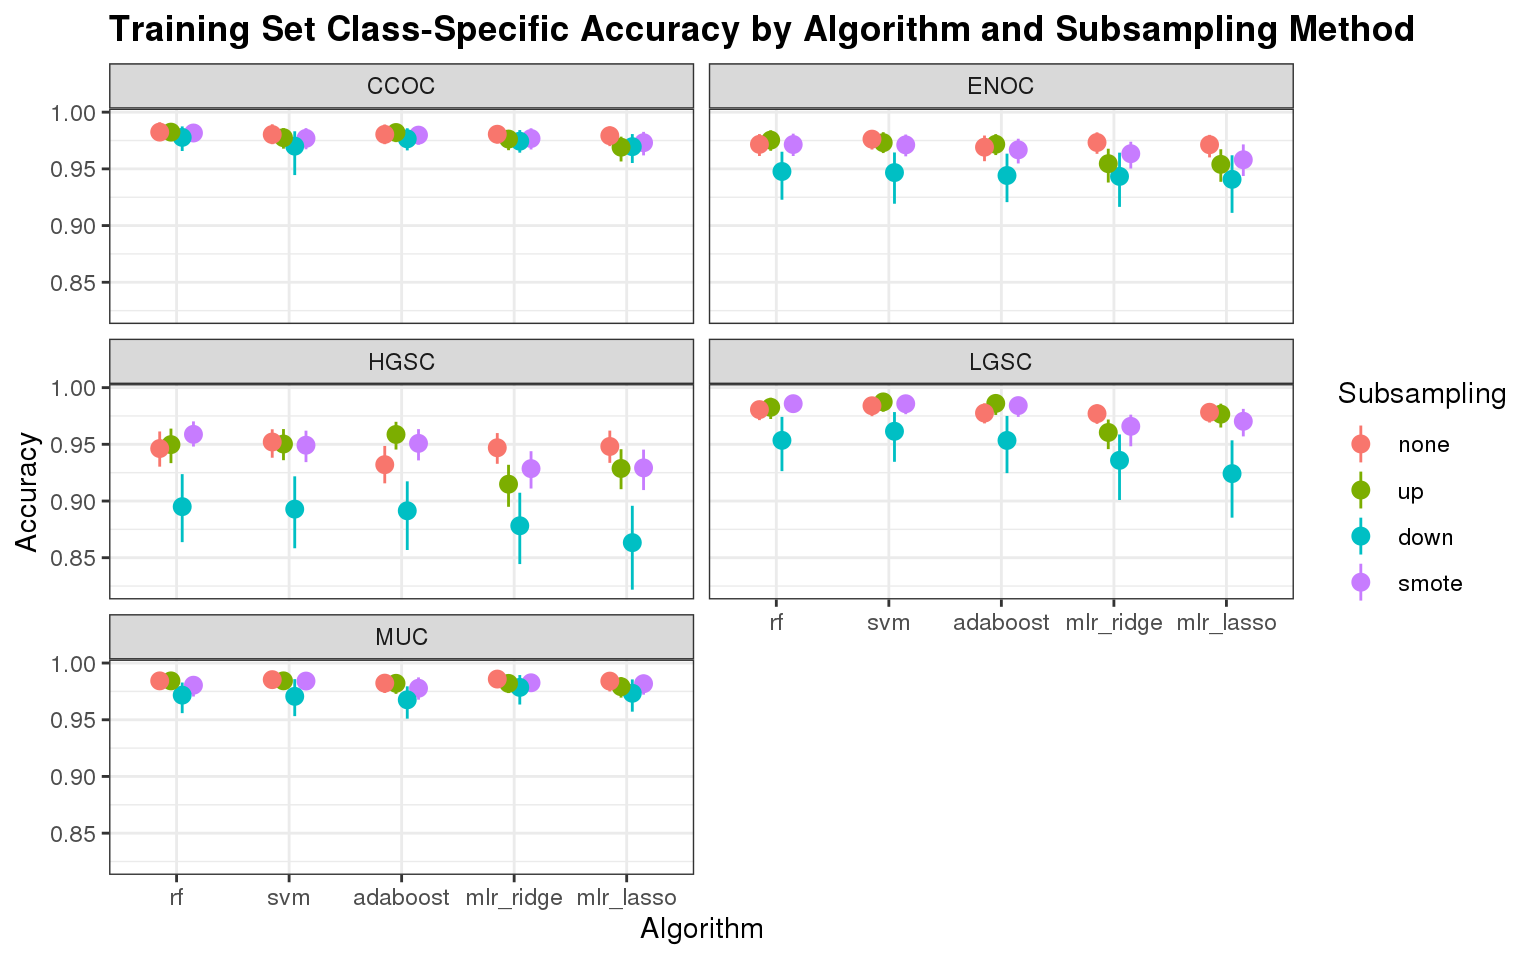
\includegraphics{OV_Histotypes_RSF_files/figure-latex/train-accuracy-class-1} 

}

\caption{Training Set Class-Specific Accuracy}\label{fig:train-accuracy-class}
\end{figure}

\begin{table}

\caption{\label{tab:train-accuracy-class-table}Training Set Class-Specific Accuracy by Algorithm and Subsampling Method}
\centering
\begin{tabular}[t]{l|l|l|l|l|l|l}
\hline
sampling & histotype & rf & svm & adaboost & mlr\_ridge & mlr\_lasso\\
\hline
none & CCOC & 0.982 & 0.98 & 0.98 & 0.981 & 0.979\\
\hline
none & ENOC & 0.972 & 0.976 & 0.969 & 0.973 & 0.971\\
\hline
none & HGSC & 0.946 & 0.952 & 0.932 & 0.947 & 0.948\\
\hline
none & LGSC & 0.981 & 0.984 & 0.978 & 0.977 & 0.978\\
\hline
none & MUC & 0.984 & 0.985 & 0.982 & 0.986 & 0.984\\
\hline
up & CCOC & 0.982 & 0.978 & 0.982 & 0.976 & 0.969\\
\hline
up & ENOC & 0.975 & 0.973 & 0.972 & 0.955 & 0.954\\
\hline
up & HGSC & 0.95 & 0.95 & 0.959 & 0.915 & 0.929\\
\hline
up & LGSC & 0.983 & \textbf{0.987} & 0.986 & 0.96 & 0.977\\
\hline
up & MUC & 0.984 & 0.984 & 0.982 & 0.982 & 0.979\\
\hline
down & CCOC & 0.978 & 0.97 & 0.976 & 0.974 & 0.97\\
\hline
down & ENOC & 0.948 & 0.947 & 0.944 & 0.943 & 0.941\\
\hline
down & HGSC & 0.895 & 0.893 & 0.891 & 0.878 & 0.863\\
\hline
down & LGSC & 0.953 & 0.962 & 0.953 & 0.936 & 0.924\\
\hline
down & MUC & 0.972 & 0.971 & 0.968 & 0.979 & 0.973\\
\hline
smote & CCOC & 0.982 & 0.977 & 0.98 & 0.977 & 0.973\\
\hline
smote & ENOC & 0.971 & 0.971 & 0.967 & 0.963 & 0.958\\
\hline
smote & HGSC & 0.959 & 0.949 & 0.951 & 0.929 & 0.929\\
\hline
smote & LGSC & 0.986 & 0.986 & 0.984 & 0.966 & 0.97\\
\hline
smote & MUC & 0.98 & 0.984 & 0.978 & 0.983 & 0.982\\
\hline
\end{tabular}
\end{table}

\hypertarget{f1-score}{%
\subsection{F1-Score}\label{f1-score}}

\begin{figure}[H]

{\centering 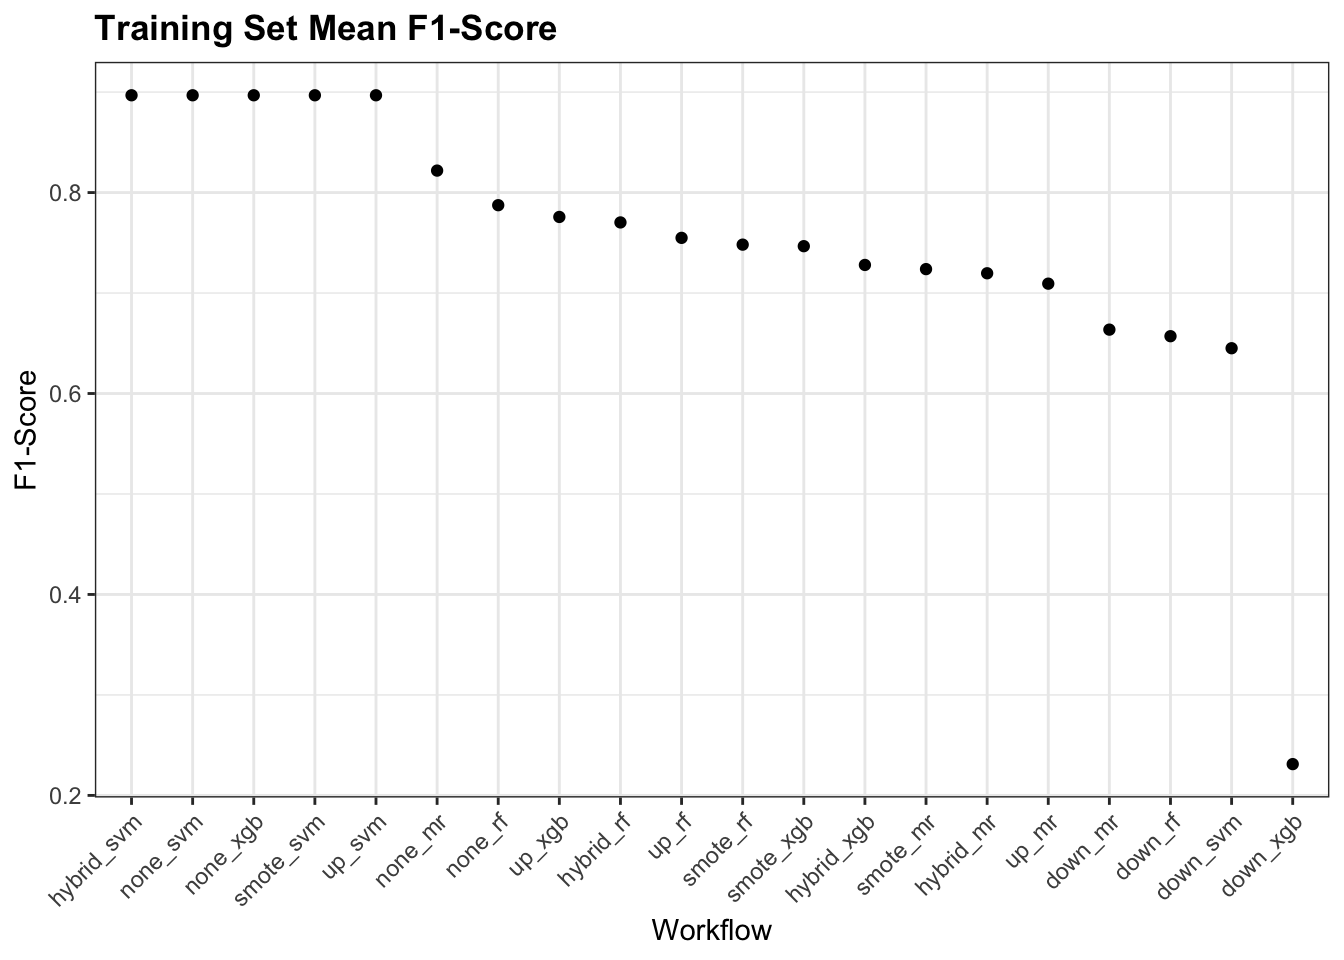
\includegraphics{OV_Histotypes_RSF_files/figure-latex/train-f1-1} 

}

\caption{Training Set F1-Score}\label{fig:train-f1}
\end{figure}

\begin{table}

\caption{\label{tab:train-f1-table}Training Set Macro-Averaged F1-Score by Algorithm and Subsampling Method}
\centering
\begin{tabular}[t]{l|l|l|l|l|l}
\hline
sampling & rf & svm & adaboost & mlr\_ridge & mlr\_lasso\\
\hline
none & 0.755 & 0.82 & 0.711 & 0.76 & 0.772\\
\hline
up & 0.791 & 0.818 & 0.821 & 0.762 & 0.759\\
\hline
down & 0.73 & 0.727 & 0.718 & 0.717 & 0.687\\
\hline
smote & \textbf{0.824} & 0.817 & 0.81 & 0.777 & 0.769\\
\hline
\end{tabular}
\end{table}

\begin{figure}[H]

{\centering 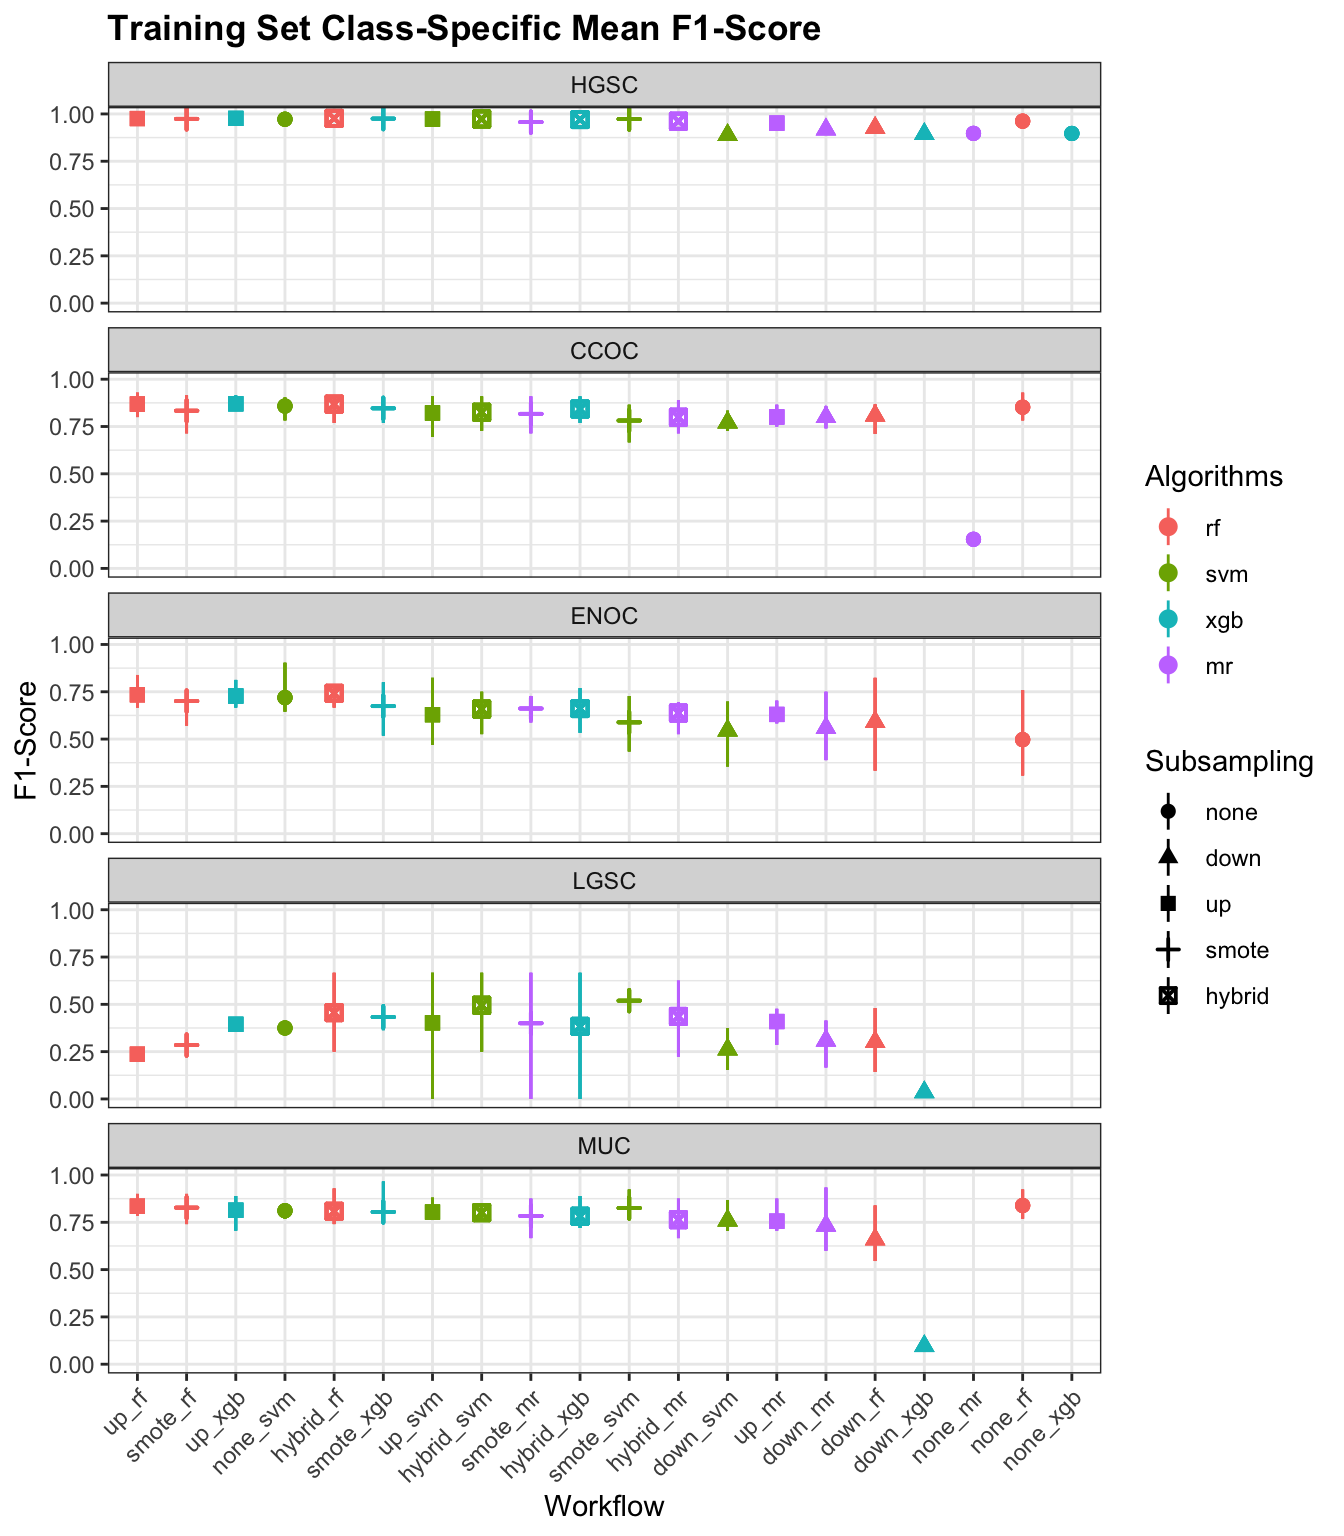
\includegraphics{OV_Histotypes_RSF_files/figure-latex/train-f1-class-1} 

}

\caption{Training Set Class-Specific F1-Score}\label{fig:train-f1-class}
\end{figure}

\begin{table}

\caption{\label{tab:train-f1-class-table}Training Set Class-Specific F1-Score by Algorithm and Subsampling Method}
\centering
\begin{tabular}[t]{l|l|l|l|l|l|l}
\hline
sampling & histotype & rf & svm & adaboost & mlr\_ridge & mlr\_lasso\\
\hline
none & CCOC & 0.866 & 0.848 & 0.846 & 0.853 & 0.843\\
\hline
none & ENOC & 0.724 & 0.786 & 0.681 & 0.757 & 0.74\\
\hline
none & HGSC & 0.967 & 0.97 & 0.959 & 0.967 & 0.968\\
\hline
none & LGSC & 0.375 & 0.667 & 0.2 & 0.353 & 0.471\\
\hline
none & MUC & 0.852 & 0.857 & 0.827 & 0.872 & 0.849\\
\hline
up & CCOC & 0.864 & 0.822 & 0.865 & 0.833 & 0.778\\
\hline
up & ENOC & 0.767 & 0.75 & 0.754 & 0.667 & 0.638\\
\hline
up & HGSC & 0.969 & 0.969 & \textbf{0.974} & 0.944 & 0.954\\
\hline
up & LGSC & 0.522 & 0.714 & 0.69 & 0.524 & 0.611\\
\hline
up & MUC & 0.852 & 0.846 & 0.839 & 0.841 & 0.808\\
\hline
down & CCOC & 0.841 & 0.79 & 0.833 & 0.821 & 0.792\\
\hline
down & ENOC & 0.641 & 0.629 & 0.615 & 0.627 & 0.605\\
\hline
down & HGSC & 0.93 & 0.928 & 0.927 & 0.917 & 0.907\\
\hline
down & LGSC & 0.487 & 0.526 & 0.481 & 0.413 & 0.368\\
\hline
down & MUC & 0.765 & 0.762 & 0.741 & 0.811 & 0.769\\
\hline
smote & CCOC & 0.862 & 0.824 & 0.85 & 0.835 & 0.813\\
\hline
smote & ENOC & 0.759 & 0.759 & 0.721 & 0.71 & 0.675\\
\hline
smote & HGSC & \textbf{0.974} & 0.968 & 0.969 & 0.953 & 0.954\\
\hline
smote & LGSC & 0.71 & 0.706 & 0.706 & 0.545 & 0.571\\
\hline
smote & MUC & 0.829 & 0.847 & 0.81 & 0.847 & 0.833\\
\hline
\end{tabular}
\end{table}

\hypertarget{kappa}{%
\subsection{Kappa}\label{kappa}}

\begin{figure}[H]

{\centering 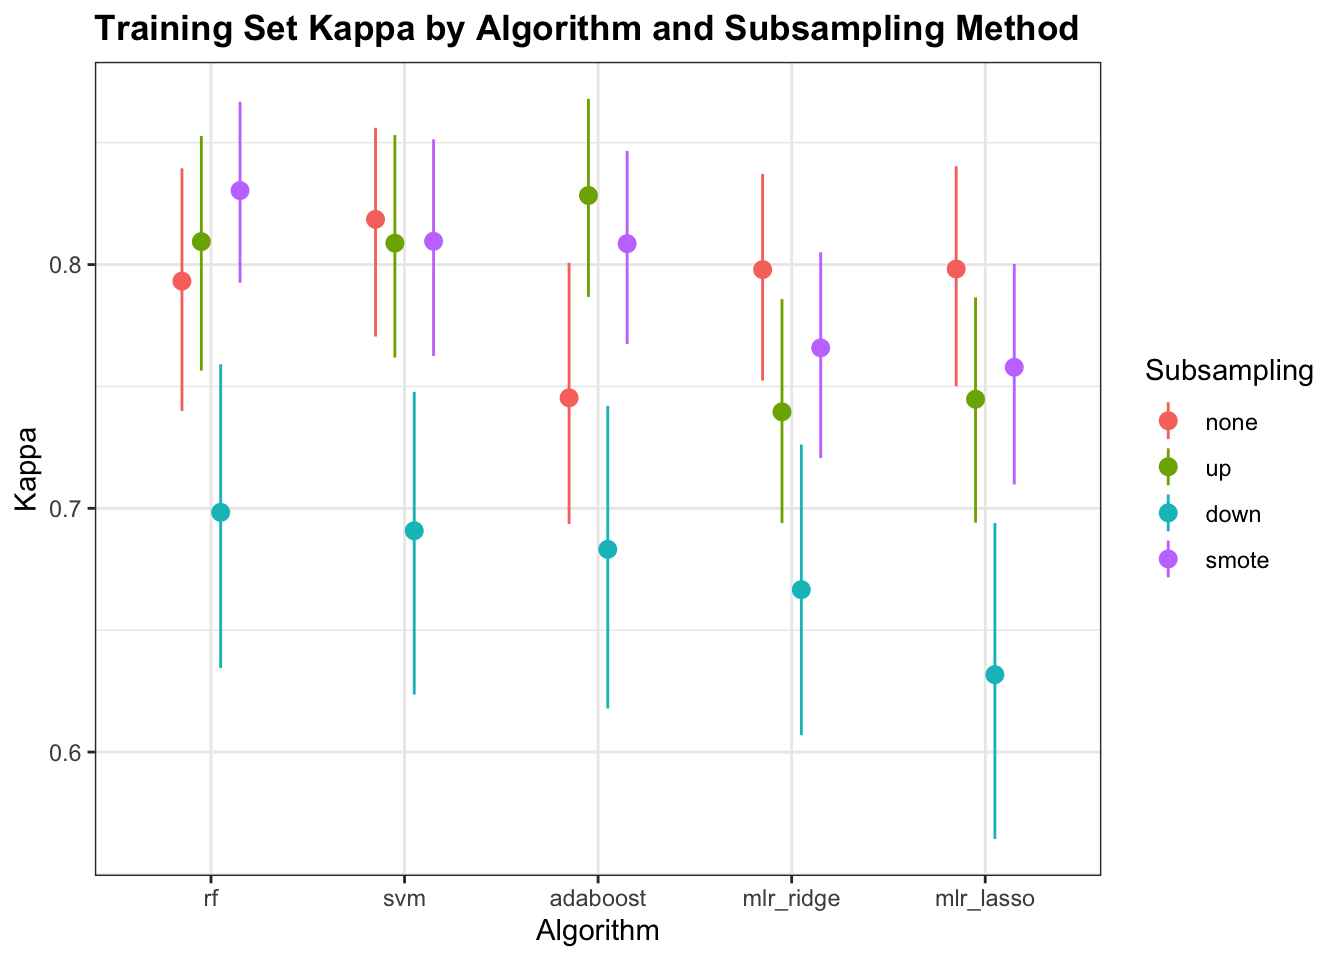
\includegraphics{OV_Histotypes_RSF_files/figure-latex/train-kappa-1} 

}

\caption{Training Set Kappa}\label{fig:train-kappa}
\end{figure}

\begin{table}

\caption{\label{tab:train-kappa-table}Training Set Kappa by Algorithm and Subsampling Method}
\centering
\begin{tabular}[t]{l|l|l|l|l|l}
\hline
sampling & rf & svm & adaboost & mlr\_ridge & mlr\_lasso\\
\hline
none & 0.793 & 0.819 & 0.745 & 0.798 & 0.798\\
\hline
up & 0.809 & 0.809 & 0.828 & 0.74 & 0.745\\
\hline
down & 0.698 & 0.691 & 0.683 & 0.667 & 0.632\\
\hline
smote & \textbf{0.83} & 0.81 & 0.809 & 0.766 & 0.758\\
\hline
\end{tabular}
\end{table}

\begin{figure}[H]

{\centering 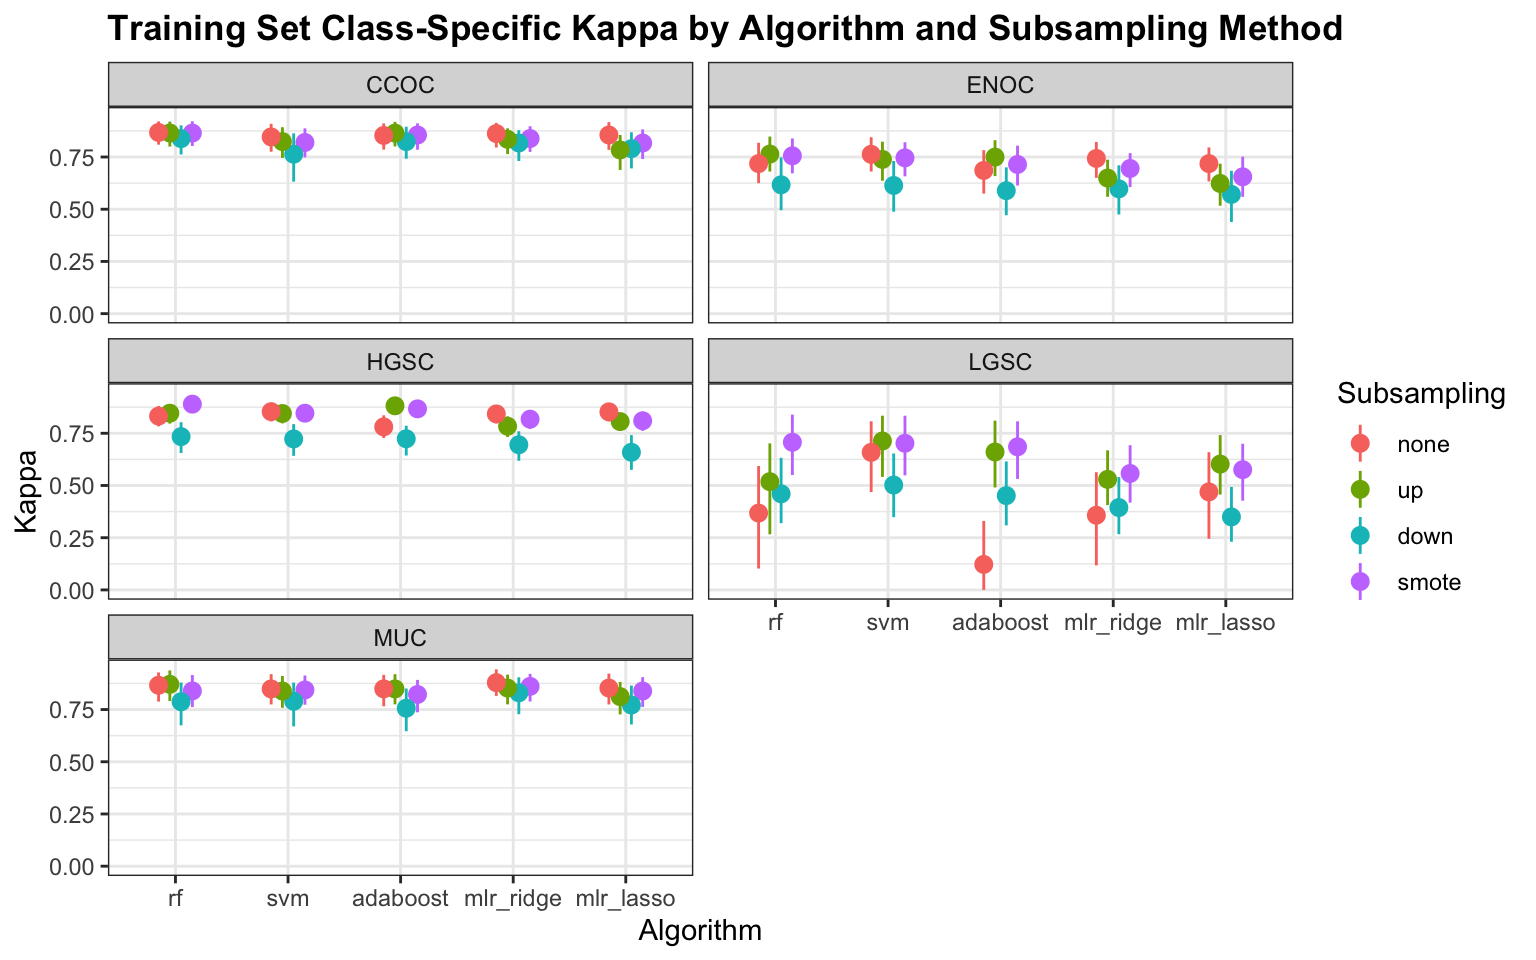
\includegraphics{OV_Histotypes_RSF_files/figure-latex/train-kappa-class-1} 

}

\caption{Training Set Class-Specific Kappa}\label{fig:train-kappa-class}
\end{figure}

\begin{table}

\caption{\label{tab:train-kappa-class-table}Training Set Class-Specific Kappa by Algorithm and Subsampling Method}
\centering
\begin{tabular}[t]{l|l|l|l|l|l|l}
\hline
sampling & histotype & rf & svm & adaboost & mlr\_ridge & mlr\_lasso\\
\hline
none & CCOC & 0.857 & 0.836 & 0.835 & 0.843 & 0.831\\
\hline
none & ENOC & 0.71 & 0.774 & 0.666 & 0.744 & 0.723\\
\hline
none & HGSC & 0.822 & 0.848 & 0.77 & 0.829 & 0.837\\
\hline
none & LGSC & 0.369 & 0.656 & 0.151 & 0.344 & 0.464\\
\hline
none & MUC & 0.844 & 0.849 & 0.818 & 0.864 & 0.839\\
\hline
up & CCOC & 0.854 & 0.812 & 0.855 & 0.82 & 0.762\\
\hline
up & ENOC & 0.753 & 0.735 & 0.739 & 0.645 & 0.614\\
\hline
up & HGSC & 0.835 & 0.839 & 0.873 & 0.768 & 0.792\\
\hline
up & LGSC & 0.514 & 0.707 & 0.682 & 0.508 & 0.599\\
\hline
up & MUC & 0.844 & 0.839 & 0.829 & 0.83 & 0.797\\
\hline
down & CCOC & 0.828 & 0.774 & 0.821 & 0.807 & 0.775\\
\hline
down & ENOC & 0.615 & 0.6 & 0.586 & 0.598 & 0.575\\
\hline
down & HGSC & 0.724 & 0.719 & 0.715 & 0.686 & 0.656\\
\hline
down & LGSC & 0.465 & 0.509 & 0.461 & 0.387 & 0.341\\
\hline
down & MUC & 0.75 & 0.746 & 0.723 & 0.798 & 0.755\\
\hline
smote & CCOC & 0.853 & 0.81 & 0.839 & 0.822 & 0.798\\
\hline
smote & ENOC & 0.744 & 0.743 & 0.704 & 0.69 & 0.651\\
\hline
smote & HGSC & \textbf{0.876} & 0.842 & 0.854 & 0.8 & 0.798\\
\hline
smote & LGSC & 0.701 & 0.697 & 0.696 & 0.528 & 0.559\\
\hline
smote & MUC & 0.817 & 0.839 & 0.797 & 0.839 & 0.824\\
\hline
\end{tabular}
\end{table}

\hypertarget{g-mean}{%
\subsection{G-mean}\label{g-mean}}

\begin{figure}[H]

{\centering 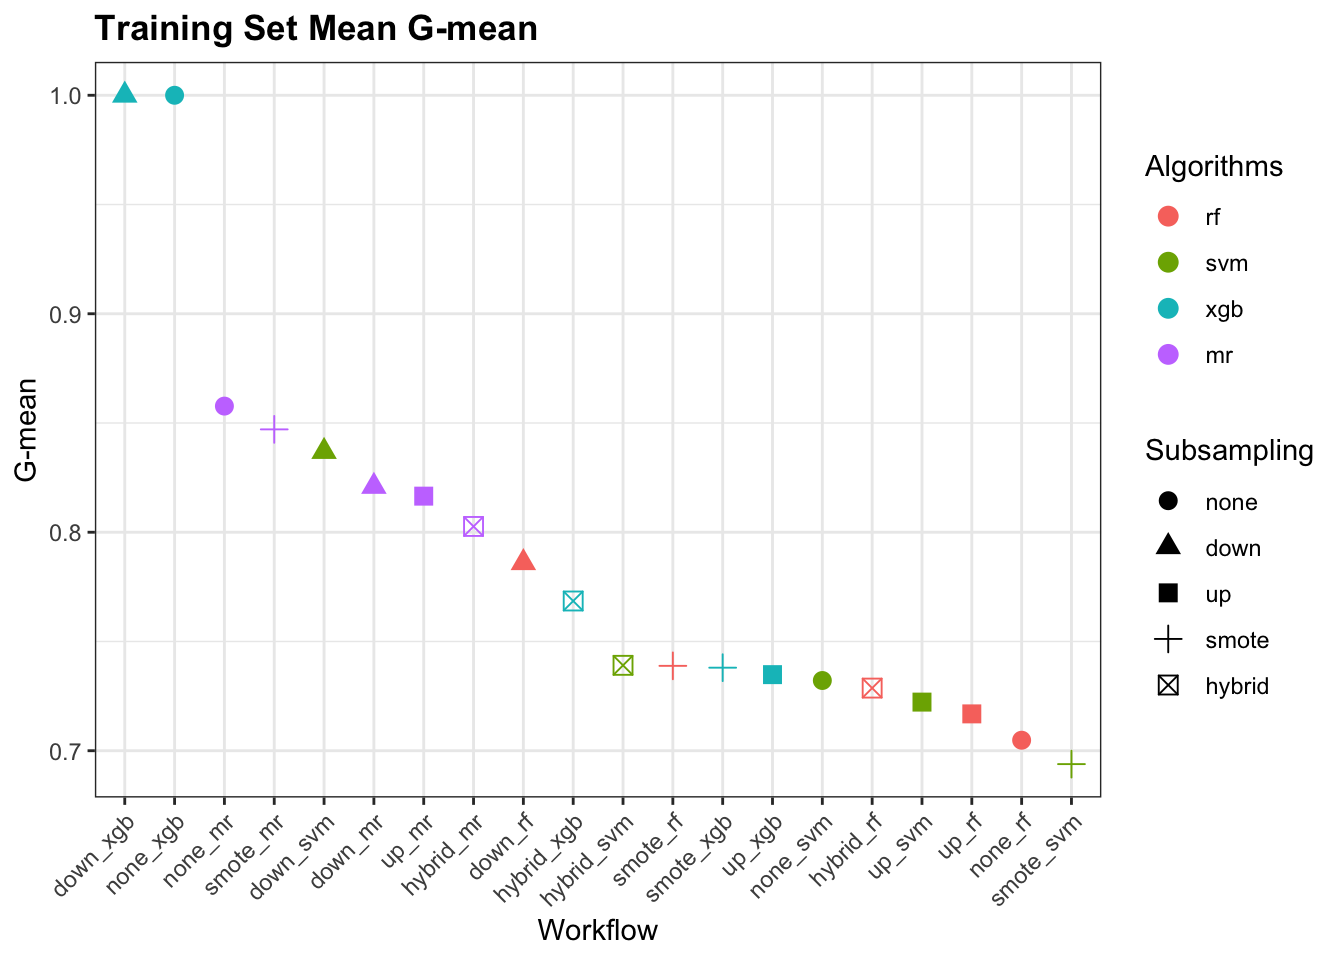
\includegraphics{OV_Histotypes_RSF_files/figure-latex/train-gmean-1} 

}

\caption{Training Set G-mean}\label{fig:train-gmean}
\end{figure}

\begin{table}

\caption{\label{tab:train-gmean-table}Training Set G-mean by Algorithm and Subsampling Method}
\centering
\begin{tabular}[t]{l|l|l|l|l|l}
\hline
sampling & rf & svm & adaboost & mlr\_ridge & mlr\_lasso\\
\hline
none & 0.632 & 0.779 & 0.497 & 0.654 & 0.71\\
\hline
up & 0.701 & 0.766 & 0.8 & \textbf{0.868} & 0.799\\
\hline
down & 0.851 & 0.843 & 0.841 & 0.856 & 0.832\\
\hline
smote & 0.828 & 0.801 & 0.831 & 0.852 & 0.835\\
\hline
\end{tabular}
\end{table}

\begin{figure}[H]

{\centering 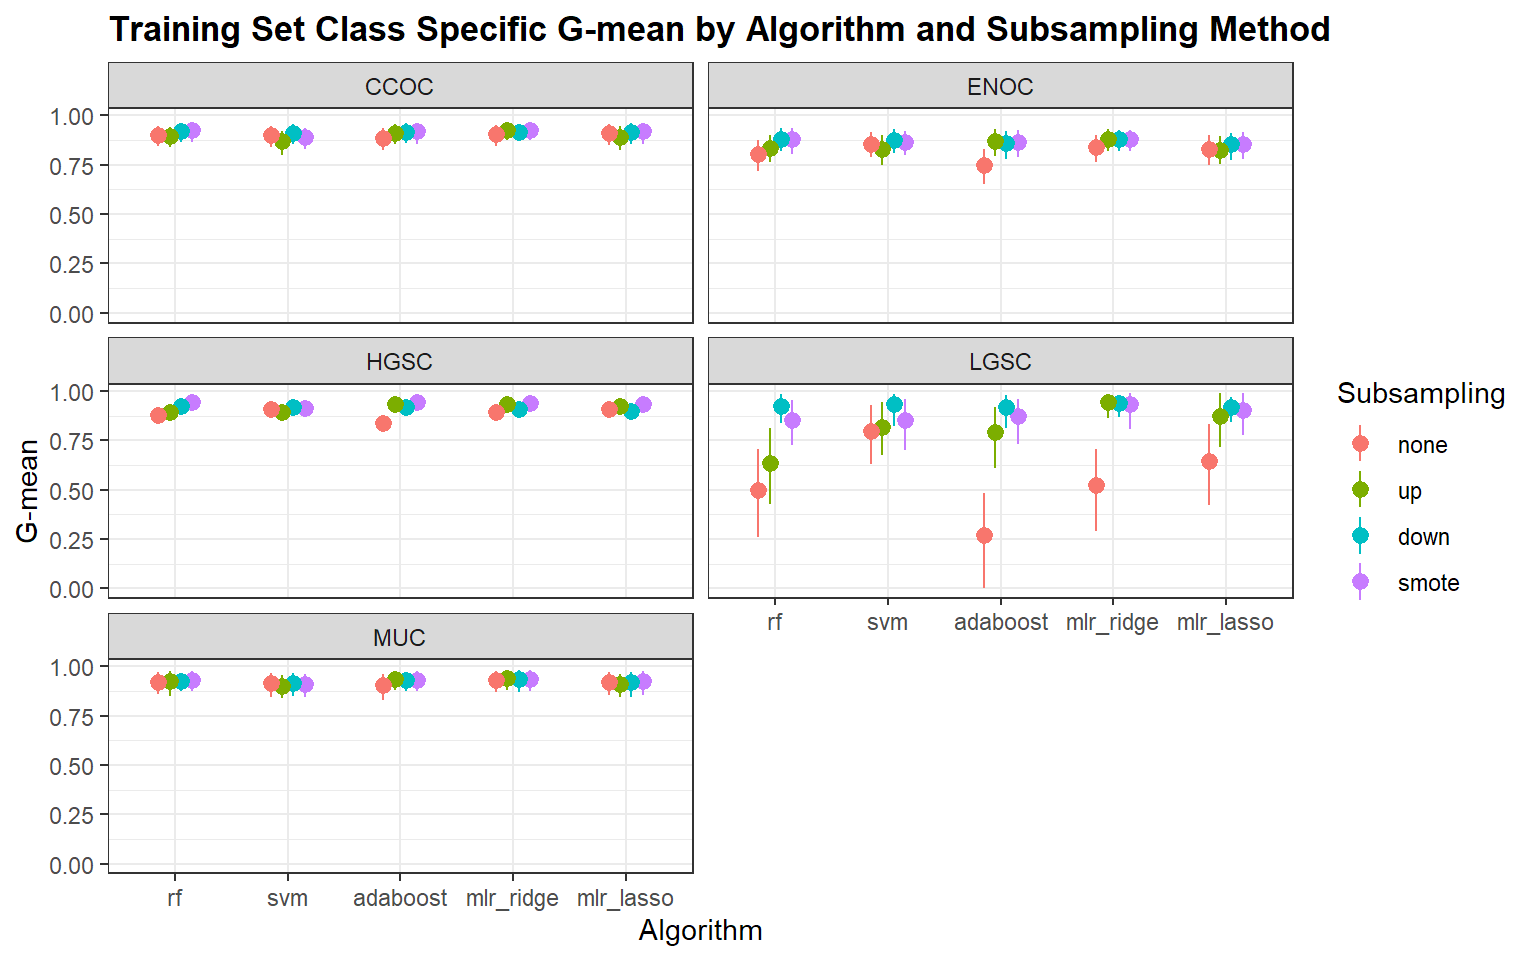
\includegraphics{OV_Histotypes_RSF_files/figure-latex/train-gmean-class-1} 

}

\caption{Training Set Class-Specific G-mean}\label{fig:train-gmean-class}
\end{figure}

\begin{table}

\caption{\label{tab:train-gmean-class-table}Training Set Class-Specific G-mean by Algorithm and Subsampling Method}
\centering
\begin{tabular}[t]{l|l|l|l|l|l|l}
\hline
sampling & histotype & rf & svm & adaboost & mlr\_ridge & mlr\_lasso\\
\hline
none & CCOC & 0.896 & 0.892 & 0.876 & 0.896 & 0.9\\
\hline
none & ENOC & 0.796 & 0.857 & 0.753 & 0.843 & 0.836\\
\hline
none & HGSC & 0.873 & 0.903 & 0.83 & 0.888 & 0.901\\
\hline
none & LGSC & 0.499 & 0.785 & 0.289 & 0.5 & 0.622\\
\hline
none & MUC & 0.912 & 0.901 & 0.881 & 0.926 & 0.918\\
\hline
up & CCOC & 0.893 & 0.864 & 0.906 & 0.921 & 0.885\\
\hline
up & ENOC & 0.835 & 0.83 & 0.86 & 0.878 & 0.831\\
\hline
up & HGSC & 0.883 & 0.891 & 0.93 & 0.93 & 0.918\\
\hline
up & LGSC & 0.612 & 0.813 & 0.794 & 0.933 & 0.867\\
\hline
up & MUC & 0.906 & 0.889 & 0.927 & 0.935 & 0.902\\
\hline
down & CCOC & 0.921 & 0.903 & 0.914 & 0.912 & 0.911\\
\hline
down & ENOC & 0.878 & 0.869 & 0.854 & 0.879 & 0.858\\
\hline
down & HGSC & 0.917 & 0.914 & 0.914 & 0.908 & 0.898\\
\hline
down & LGSC & 0.912 & 0.916 & 0.909 & 0.928 & 0.908\\
\hline
down & MUC & 0.921 & 0.919 & 0.923 & 0.927 & 0.912\\
\hline
smote & CCOC & 0.92 & 0.885 & 0.913 & 0.919 & 0.916\\
\hline
smote & ENOC & 0.875 & 0.865 & 0.861 & 0.874 & 0.858\\
\hline
smote & HGSC & \textbf{0.943} & 0.912 & 0.939 & 0.933 & 0.929\\
\hline
smote & LGSC & 0.842 & 0.841 & 0.871 & 0.91 & 0.886\\
\hline
smote & MUC & 0.927 & 0.9 & 0.928 & 0.933 & 0.926\\
\hline
\end{tabular}
\end{table}

\hypertarget{two-step-training-set}{%
\section{Two-Step Training Set}\label{two-step-training-set}}

\hypertarget{accuracy-1}{%
\subsection{Accuracy}\label{accuracy-1}}

\begin{figure}[H]

{\centering 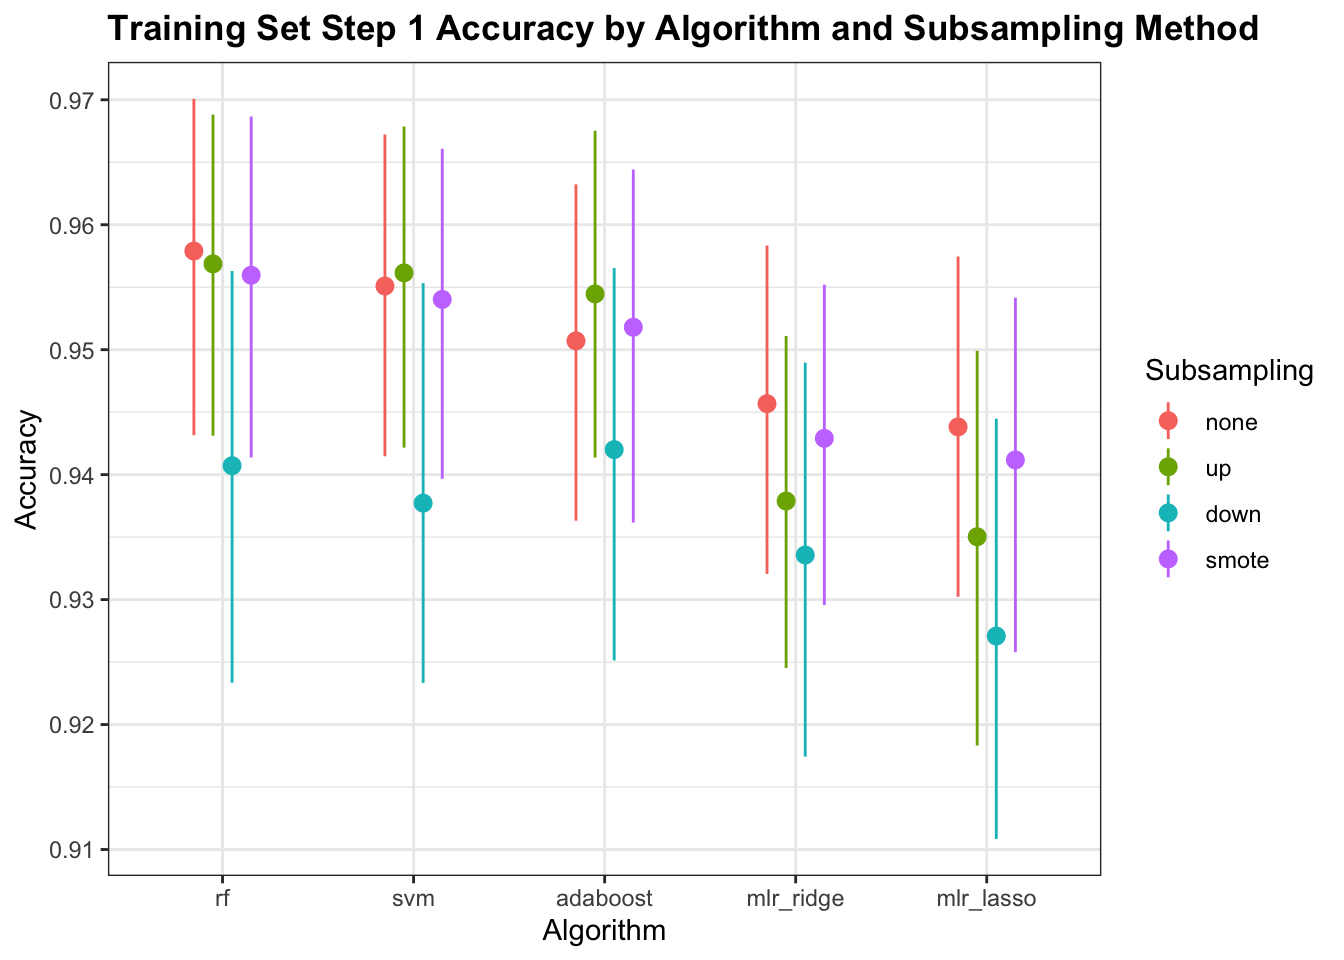
\includegraphics{OV_Histotypes_RSF_files/figure-latex/train-step1-accuracy-1} 

}

\caption{Training Set Step 1 Accuracy}\label{fig:train-step1-accuracy}
\end{figure}

\begin{figure}[H]

{\centering 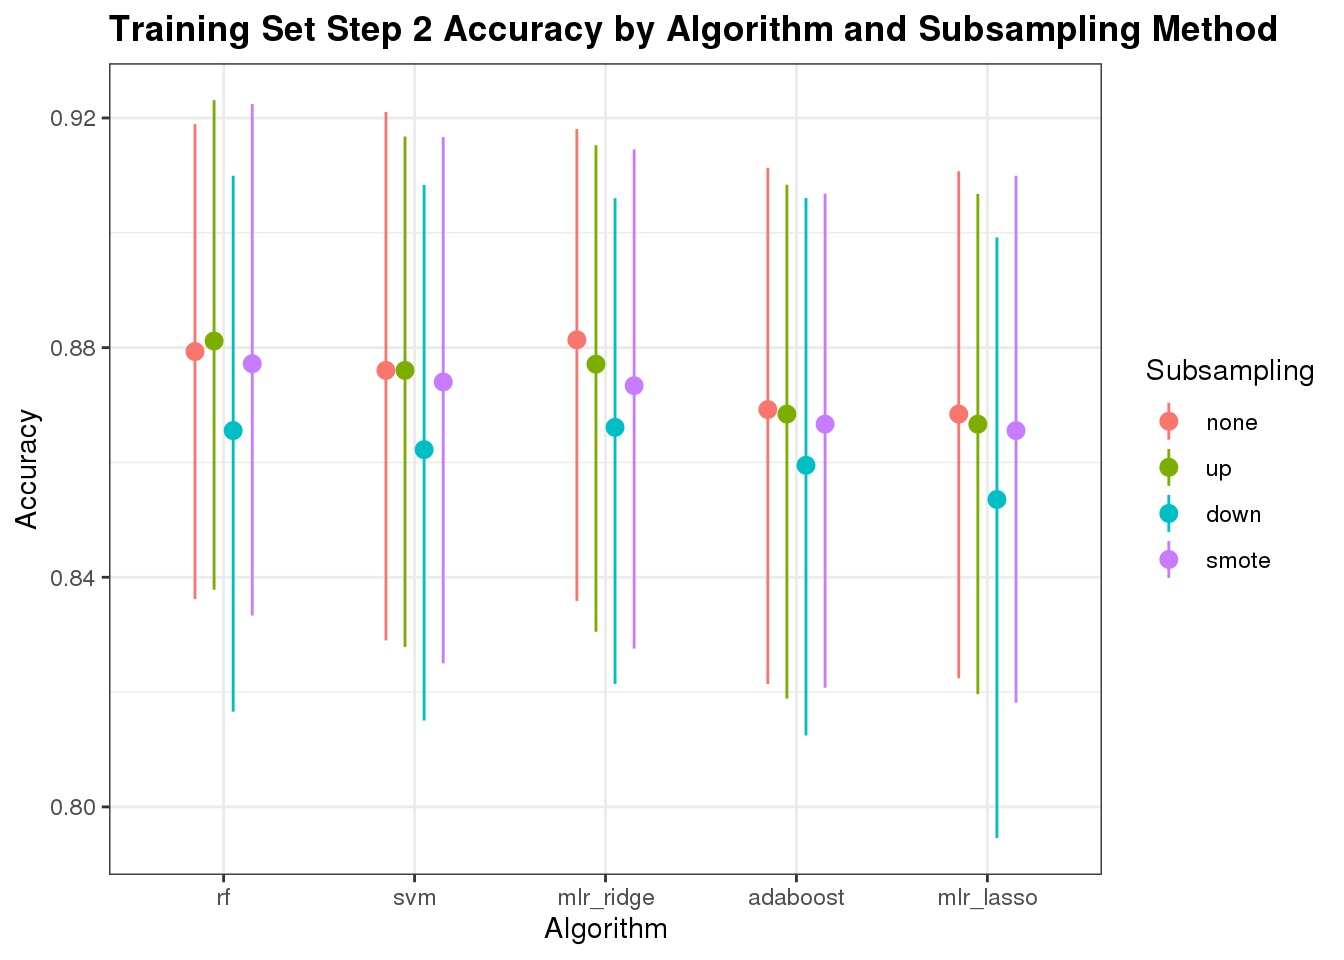
\includegraphics{OV_Histotypes_RSF_files/figure-latex/train-step2-accuracy-1} 

}

\caption{Training Set Step 2 Accuracy}\label{fig:train-step2-accuracy}
\end{figure}

\begin{table}

\caption{\label{tab:train-step1-accuracy-table}Training Set Step 1 Accuracy by Algorithm and Subsampling Method}
\centering
\begin{tabular}[t]{l|l|l|l|l|l}
\hline
sampling & rf & svm & adaboost & mlr\_ridge & mlr\_lasso\\
\hline
none & \textbf{0.958} & 0.955 & 0.951 & 0.946 & 0.944\\
\hline
up & 0.957 & 0.956 & 0.954 & 0.938 & 0.935\\
\hline
down & 0.941 & 0.938 & 0.942 & 0.934 & 0.927\\
\hline
smote & 0.956 & 0.954 & 0.952 & 0.943 & 0.941\\
\hline
\end{tabular}
\end{table}

\begin{table}

\caption{\label{tab:train-step2-accuracy-table}Training Set Step 2 Accuracy by Algorithm and Subsampling Method}
\centering
\begin{tabular}[t]{l|l|l|l|l|l}
\hline
sampling & rf & svm & mlr\_ridge & adaboost & mlr\_lasso\\
\hline
none & 0.879 & 0.876 & \textbf{0.881} & 0.869 & 0.868\\
\hline
up & \textbf{0.881} & 0.876 & 0.877 & 0.868 & 0.867\\
\hline
down & 0.866 & 0.862 & 0.866 & 0.86 & 0.854\\
\hline
smote & 0.877 & 0.874 & 0.873 & 0.867 & 0.866\\
\hline
\end{tabular}
\end{table}

\begin{figure}[H]

{\centering 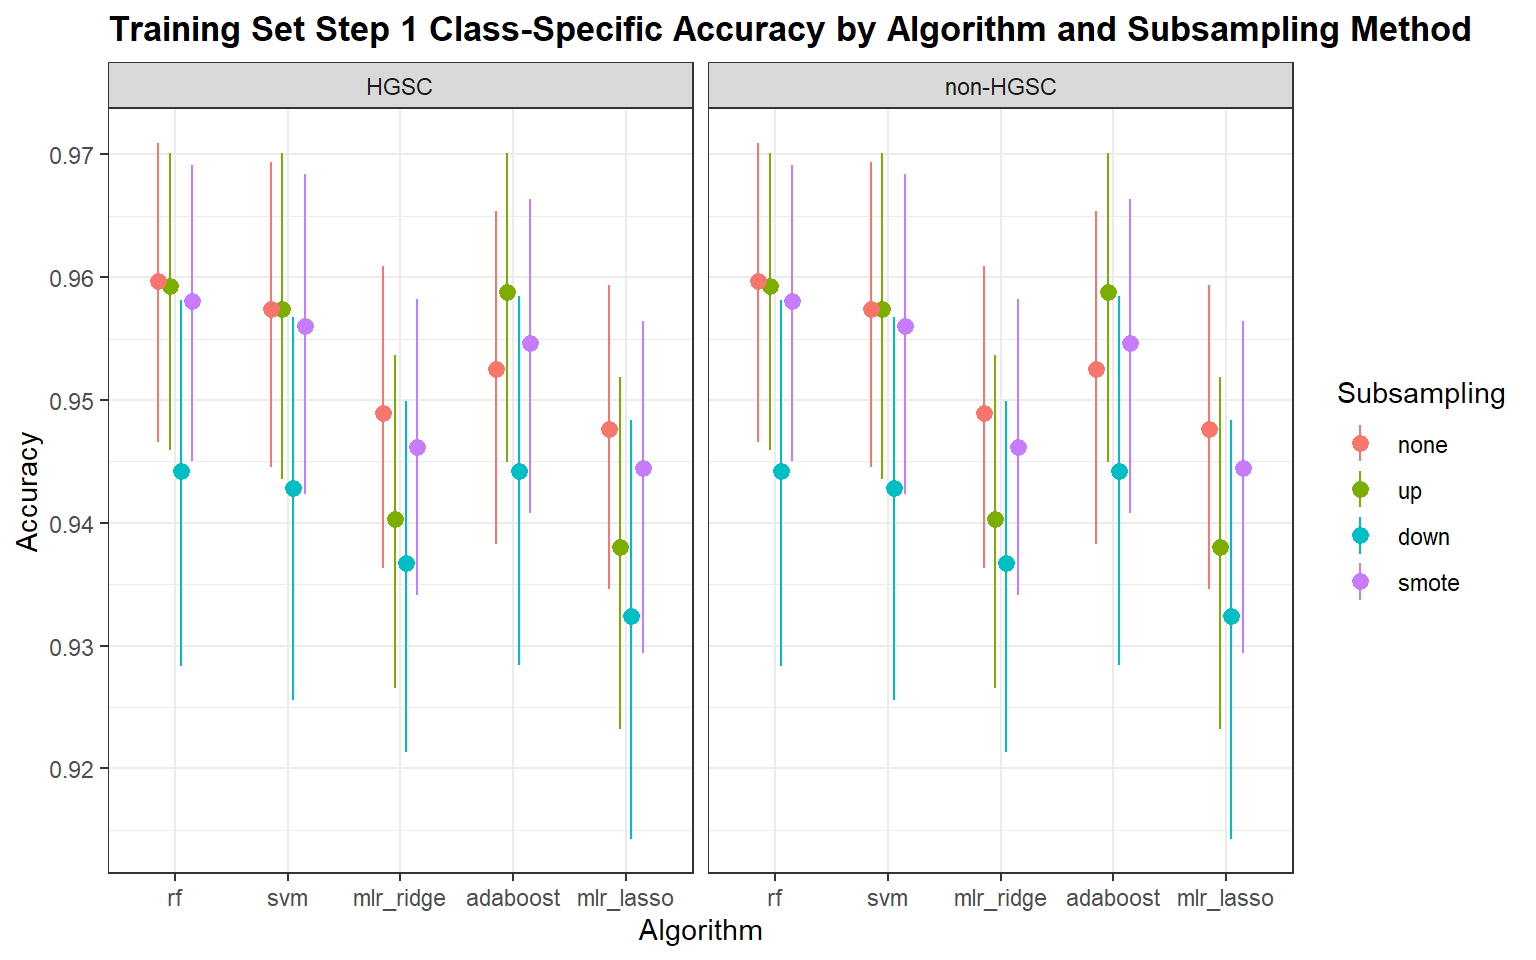
\includegraphics{OV_Histotypes_RSF_files/figure-latex/train-step1-accuracy-class-1} 

}

\caption{Training Set Step 1 Class-Specific Accuracy}\label{fig:train-step1-accuracy-class}
\end{figure}

\begin{figure}[H]

{\centering 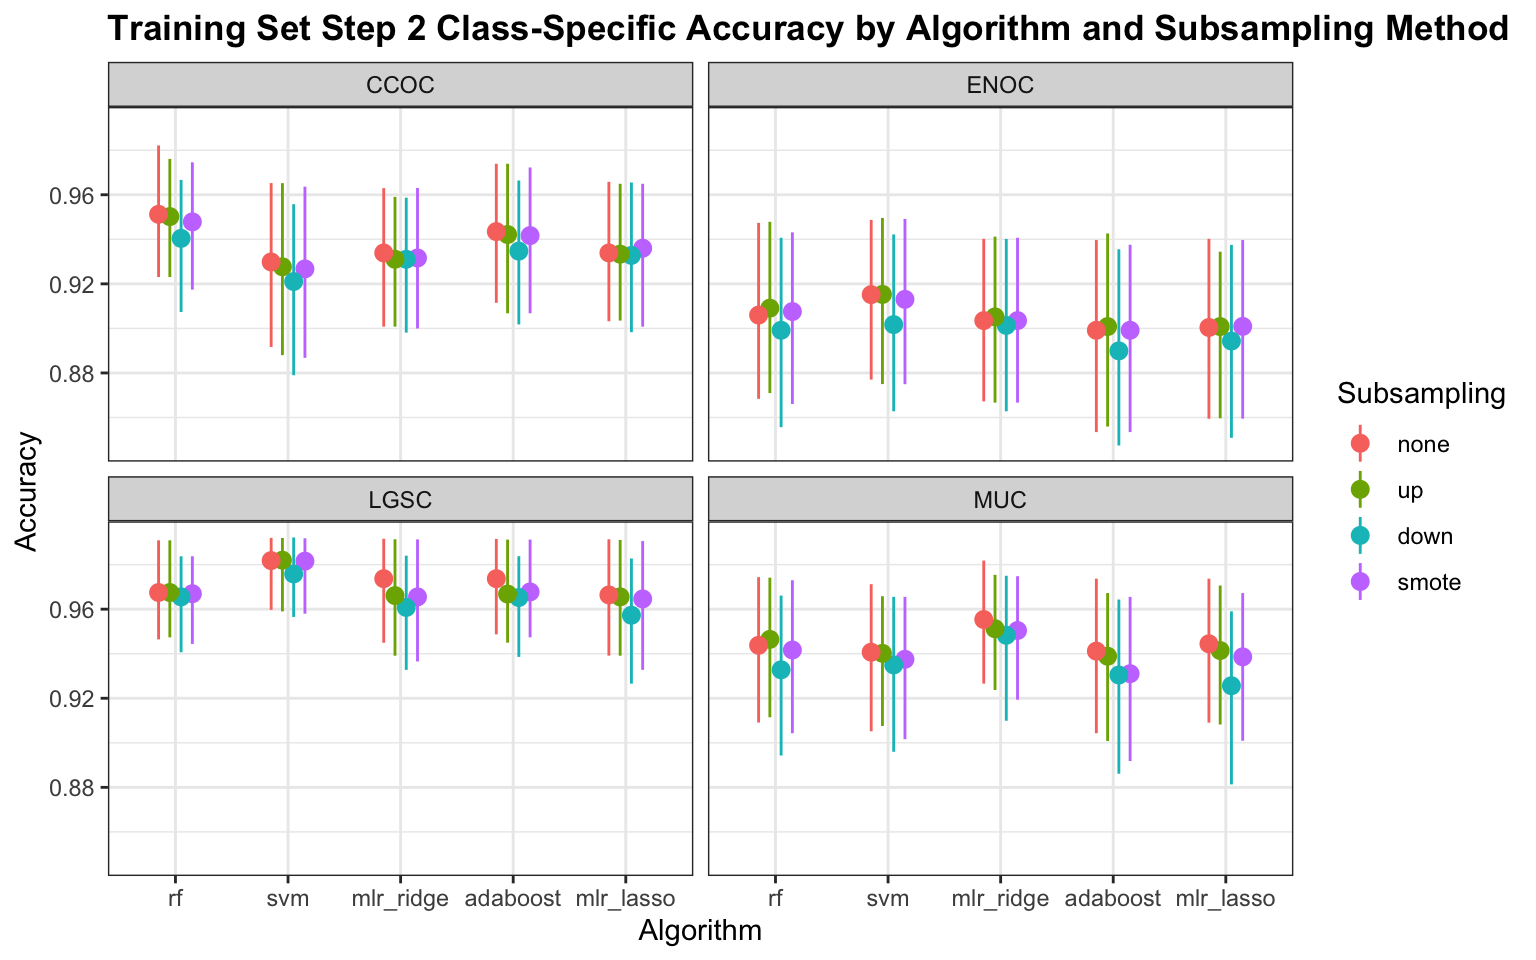
\includegraphics{OV_Histotypes_RSF_files/figure-latex/train-step2-accuracy-class-1} 

}

\caption{Training Set Step 2 Class-Specific Accuracy}\label{fig:train-step2-accuracy-class}
\end{figure}

\begin{table}

\caption{\label{tab:train-step1-accuracy-class-table}Training Set Step 1 Class-Specific Accuracy by Algorithm and Subsampling Method}
\centering
\begin{tabular}[t]{l|l|l|l|l|l|l}
\hline
sampling & histotype & rf & svm & mlr\_ridge & adaboost & mlr\_lasso\\
\hline
none & HGSC & \textbf{0.958} & 0.955 & 0.946 & 0.951 & 0.944\\
\hline
none & non-HGSC & \textbf{0.958} & 0.955 & 0.946 & 0.951 & 0.944\\
\hline
up & HGSC & 0.957 & 0.956 & 0.938 & 0.954 & 0.935\\
\hline
up & non-HGSC & 0.957 & 0.956 & 0.938 & 0.954 & 0.935\\
\hline
down & HGSC & 0.941 & 0.938 & 0.934 & 0.942 & 0.927\\
\hline
down & non-HGSC & 0.941 & 0.938 & 0.934 & 0.942 & 0.927\\
\hline
smote & HGSC & 0.956 & 0.954 & 0.943 & 0.952 & 0.941\\
\hline
smote & non-HGSC & 0.956 & 0.954 & 0.943 & 0.952 & 0.941\\
\hline
\end{tabular}
\end{table}

\begin{table}

\caption{\label{tab:train-step2-accuracy-class-table}Training Set Step 2 Class-Specific Accuracy by Algorithm and Subsampling Method}
\centering
\begin{tabular}[t]{l|l|l|l|l|l|l}
\hline
sampling & histotype & rf & svm & mlr\_ridge & adaboost & mlr\_lasso\\
\hline
none & CCOC & 0.948 & 0.928 & 0.936 & 0.942 & 0.933\\
\hline
none & ENOC & 0.901 & 0.912 & 0.903 & 0.894 & 0.899\\
\hline
none & LGSC & 0.968 & \textbf{0.982} & 0.973 & 0.972 & 0.966\\
\hline
none & MUC & 0.942 & 0.936 & 0.95 & 0.931 & 0.94\\
\hline
up & CCOC & 0.948 & 0.926 & 0.934 & 0.939 & 0.933\\
\hline
up & ENOC & 0.903 & 0.912 & 0.904 & 0.895 & 0.898\\
\hline
up & LGSC & 0.967 & \textbf{0.982} & 0.966 & 0.968 & 0.965\\
\hline
up & MUC & 0.943 & 0.935 & 0.948 & 0.934 & 0.938\\
\hline
down & CCOC & 0.939 & 0.919 & 0.932 & 0.934 & 0.932\\
\hline
down & ENOC & 0.894 & 0.901 & 0.899 & 0.888 & 0.895\\
\hline
down & LGSC & 0.966 & 0.976 & 0.958 & 0.966 & 0.958\\
\hline
down & MUC & 0.937 & 0.93 & 0.942 & 0.93 & 0.927\\
\hline
smote & CCOC & 0.943 & 0.926 & 0.934 & 0.938 & 0.933\\
\hline
smote & ENOC & 0.903 & 0.911 & 0.904 & 0.895 & 0.899\\
\hline
smote & LGSC & 0.967 & 0.976 & 0.964 & 0.973 & 0.964\\
\hline
smote & MUC & 0.943 & 0.935 & 0.947 & 0.933 & 0.936\\
\hline
\end{tabular}
\end{table}

\hypertarget{f1-score-1}{%
\subsection{F1-Score}\label{f1-score-1}}

\begin{figure}[H]

{\centering 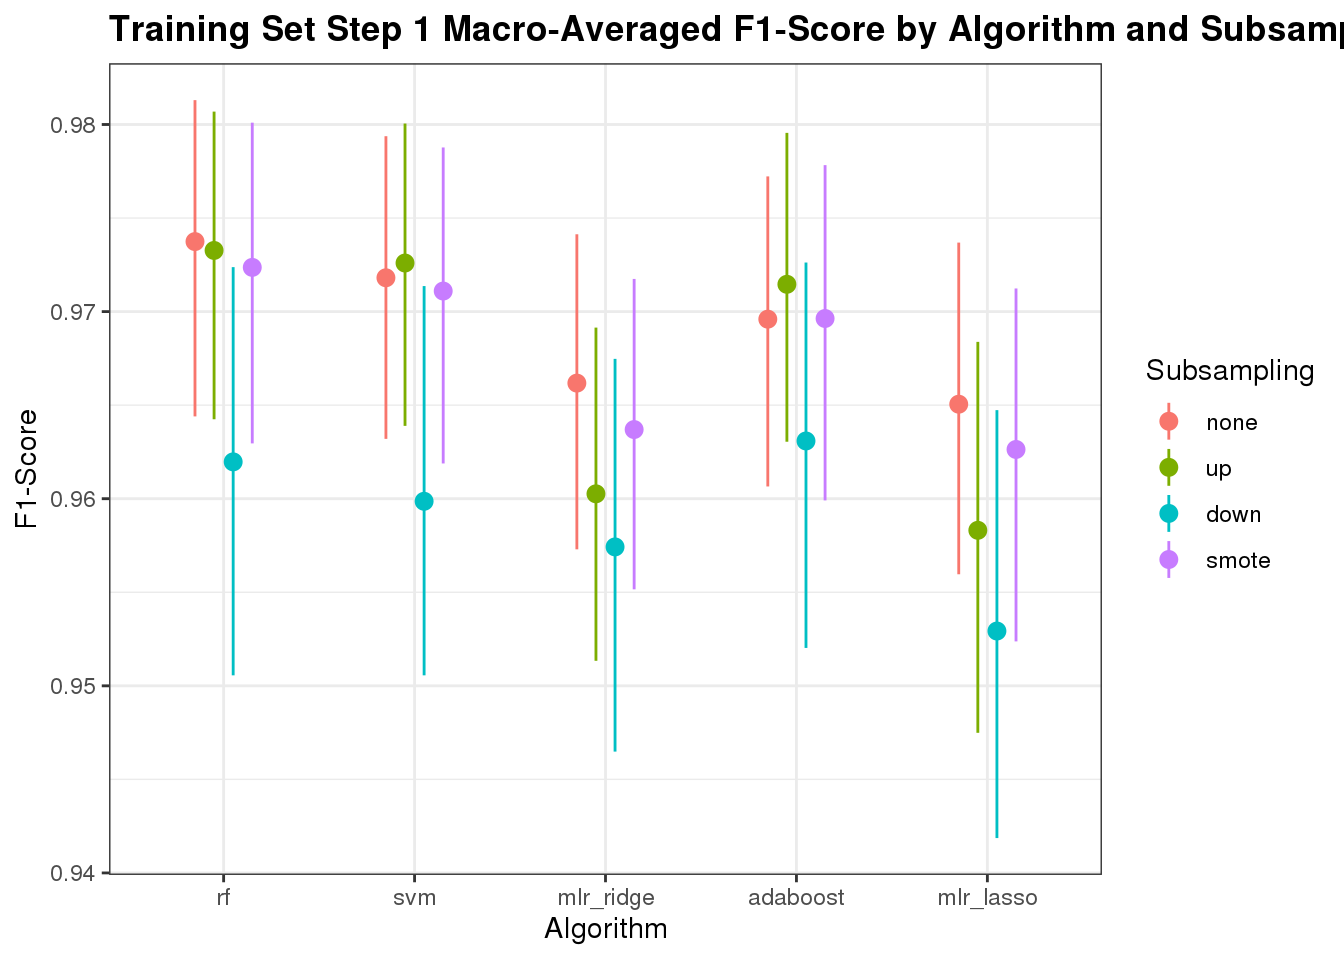
\includegraphics{OV_Histotypes_RSF_files/figure-latex/train-step1-f1-1} 

}

\caption{Training Set Step 1 F1-Score}\label{fig:train-step1-f1}
\end{figure}

\begin{figure}[H]

{\centering 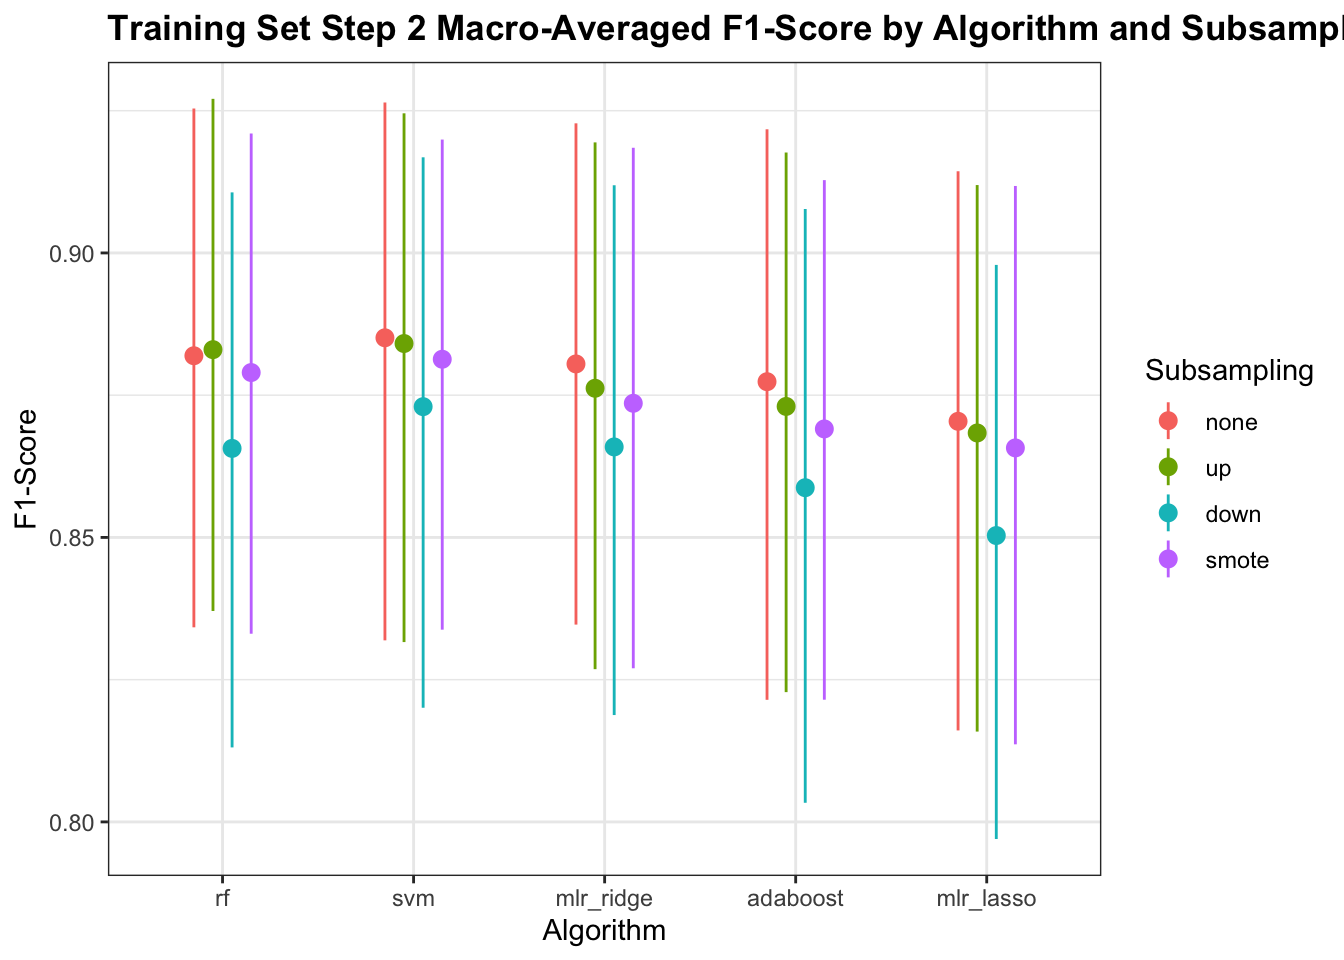
\includegraphics{OV_Histotypes_RSF_files/figure-latex/train-step2-f1-1} 

}

\caption{Training Set Step 2 F1-Score}\label{fig:train-step2-f1}
\end{figure}

\begin{table}

\caption{\label{tab:train-step1-f1-table}Training Set Step 1 Macro-Averaged F1-Score by Algorithm and Subsampling Method}
\centering
\begin{tabular}[t]{l|l|l|l|l|l}
\hline
sampling & rf & svm & mlr\_ridge & adaboost & mlr\_lasso\\
\hline
none & \textbf{0.974} & 0.972 & 0.966 & 0.97 & 0.965\\
\hline
up & 0.973 & 0.973 & 0.96 & 0.971 & 0.958\\
\hline
down & 0.962 & 0.96 & 0.957 & 0.963 & 0.953\\
\hline
smote & 0.972 & 0.971 & 0.964 & 0.97 & 0.963\\
\hline
\end{tabular}
\end{table}

\begin{table}

\caption{\label{tab:train-step2-f1-table}Training Set Step 2 Macro-Averaged F1-Score by Algorithm and Subsampling Method}
\centering
\begin{tabular}[t]{l|l|l|l|l|l}
\hline
sampling & rf & svm & mlr\_ridge & adaboost & mlr\_lasso\\
\hline
none & 0.879 & \textbf{0.88} & 0.879 & 0.869 & 0.865\\
\hline
up & 0.879 & \textbf{0.88} & 0.873 & 0.869 & 0.862\\
\hline
down & 0.865 & 0.867 & 0.861 & 0.858 & 0.848\\
\hline
smote & 0.877 & 0.878 & 0.871 & 0.866 & 0.862\\
\hline
\end{tabular}
\end{table}

\begin{figure}[H]

{\centering 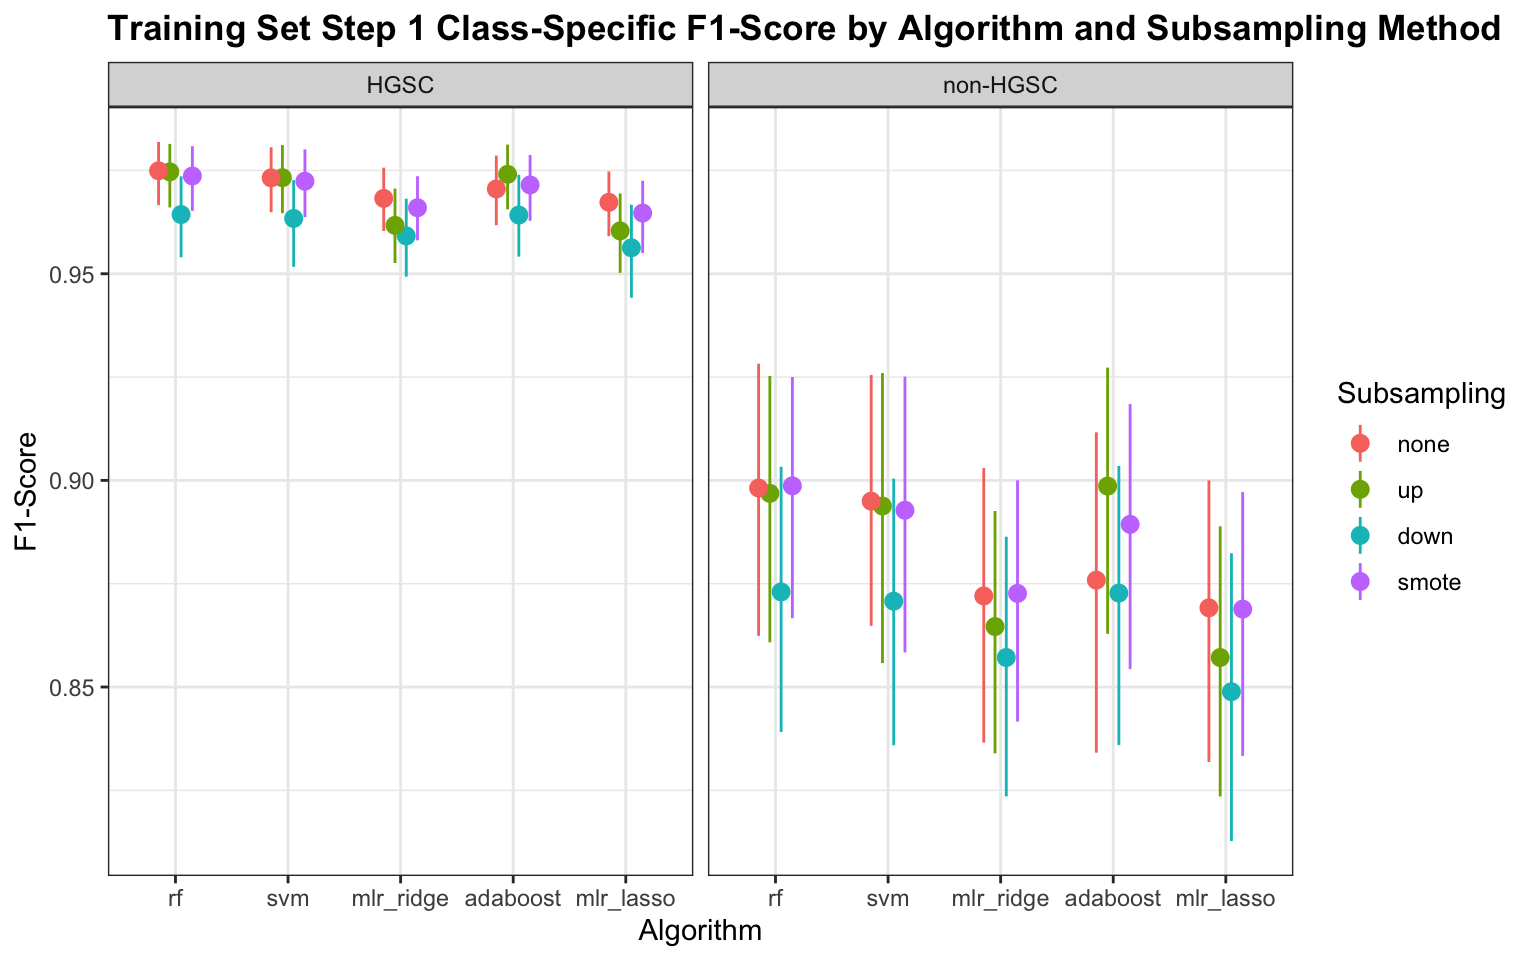
\includegraphics{OV_Histotypes_RSF_files/figure-latex/train-step1-f1-class-1} 

}

\caption{Training Set Step 1 Class-Specific F1-Score}\label{fig:train-step1-f1-class}
\end{figure}

\begin{figure}[H]

{\centering 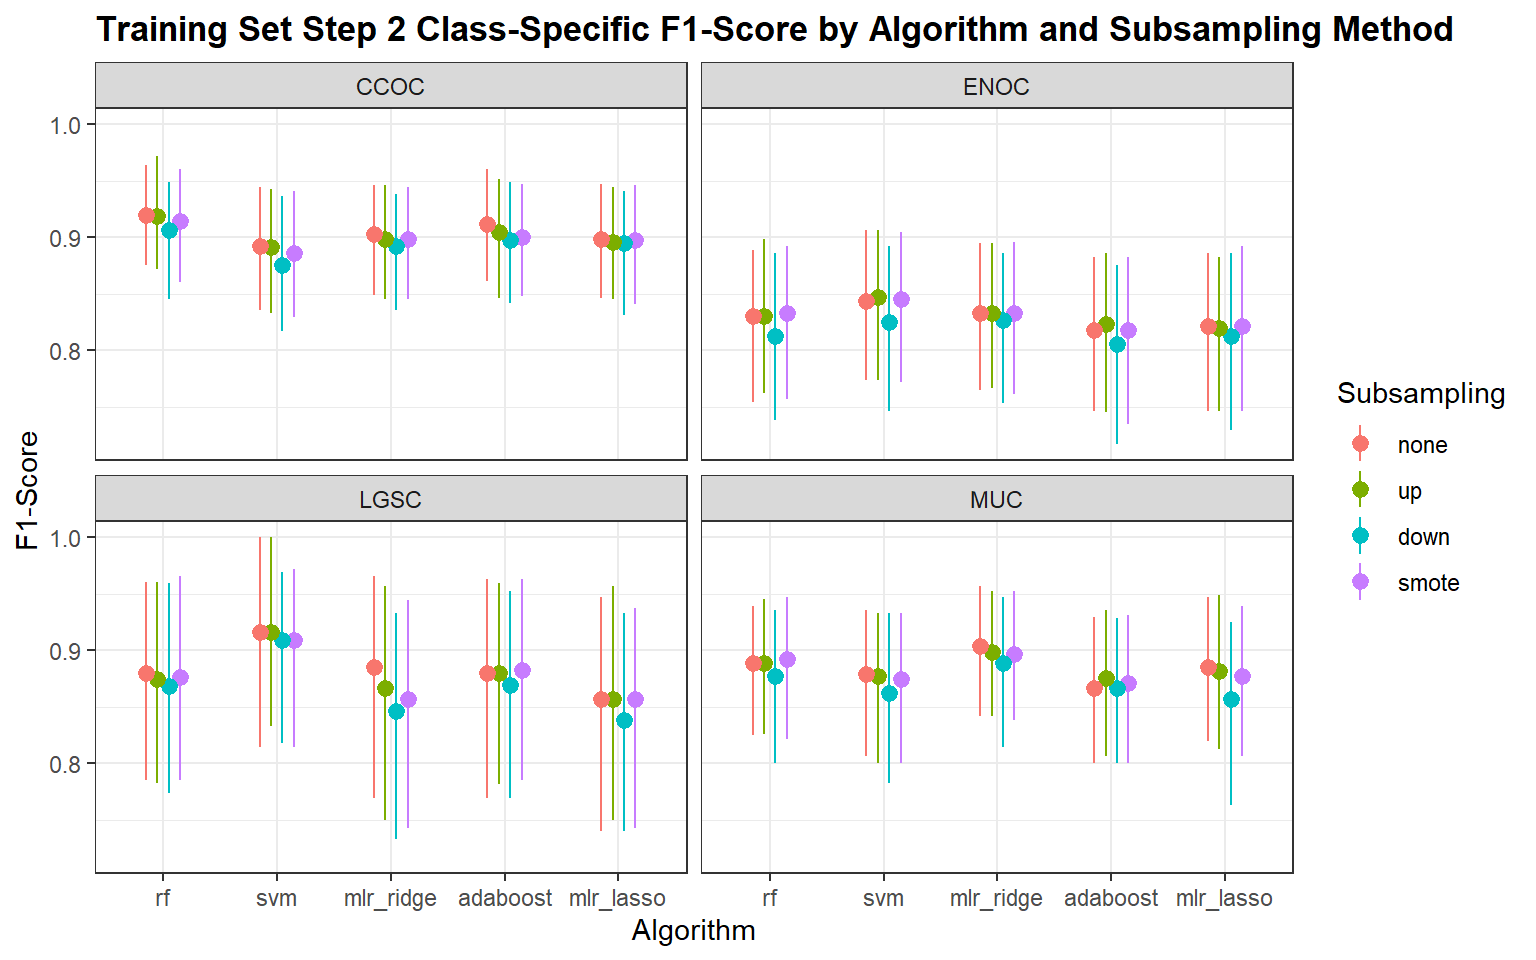
\includegraphics{OV_Histotypes_RSF_files/figure-latex/train-step2-f1-class-1} 

}

\caption{Training Set Step 2 Class-Specific F1-Score}\label{fig:train-step2-f1-class}
\end{figure}

\begin{center}\includegraphics{OV_Histotypes_RSF_files/figure-latex/train-step1-f1-class-table-1} \end{center}

\begin{center}\includegraphics{OV_Histotypes_RSF_files/figure-latex/train-step2-f1-class-table-1} \end{center}

\hypertarget{kappa-1}{%
\subsection{Kappa}\label{kappa-1}}

\begin{figure}[H]

{\centering 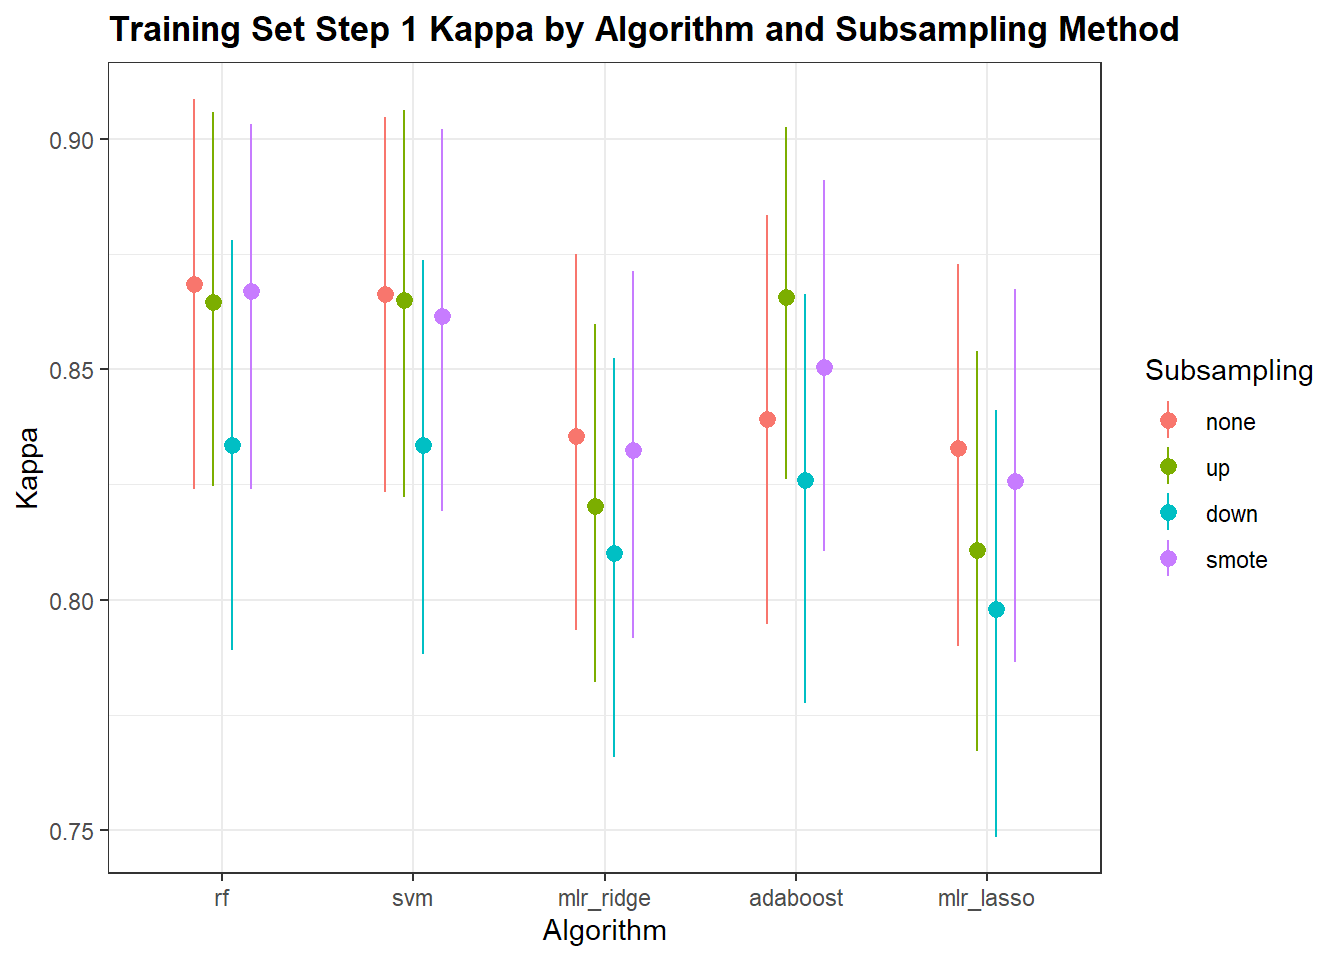
\includegraphics{OV_Histotypes_RSF_files/figure-latex/train-step1-kappa-1} 

}

\caption{Training Set Step 1 Kappa}\label{fig:train-step1-kappa}
\end{figure}

\begin{figure}[H]

{\centering 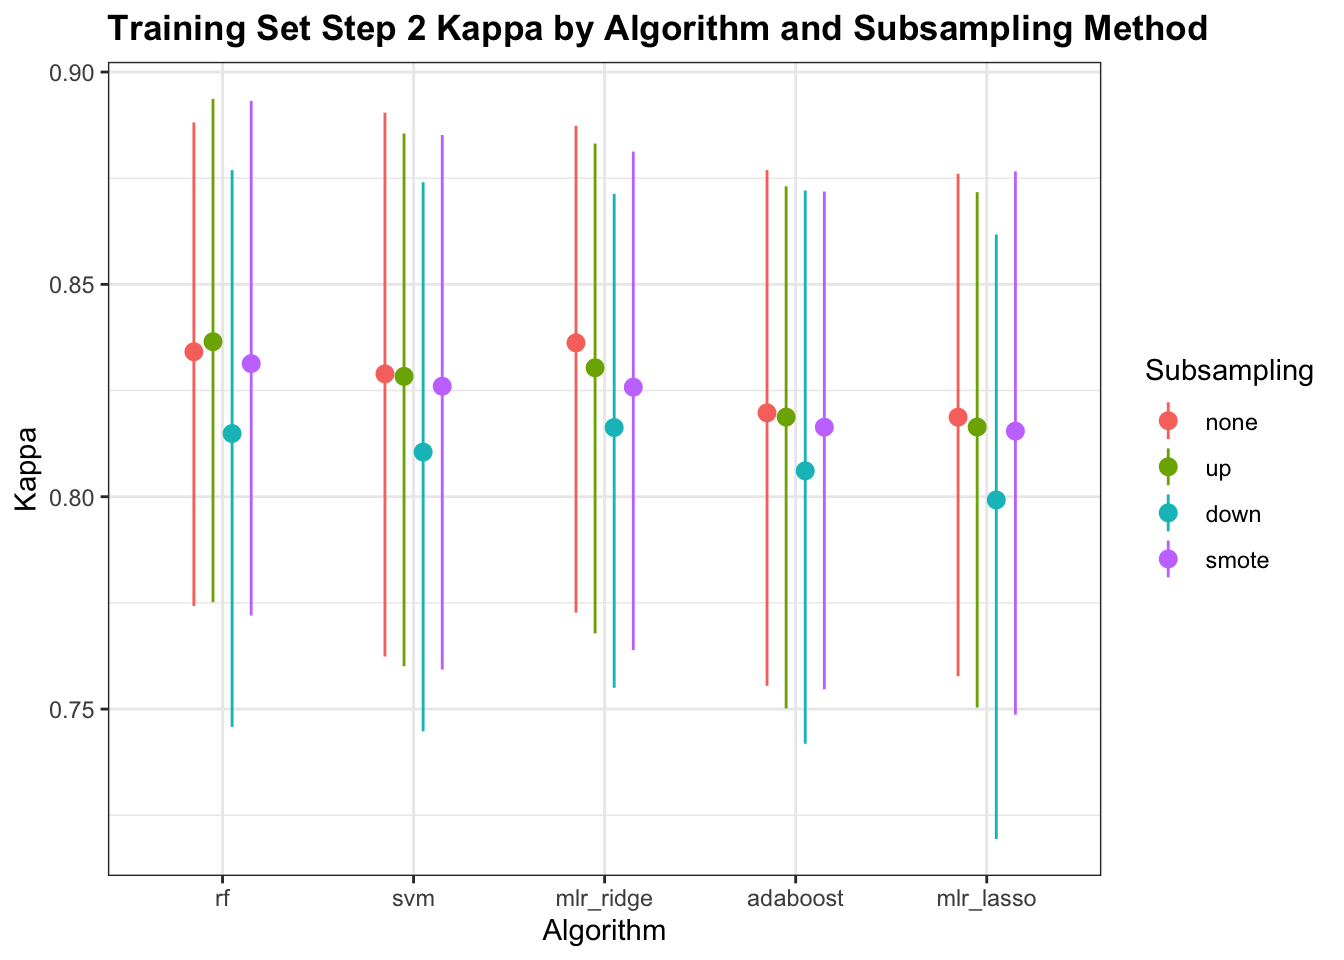
\includegraphics{OV_Histotypes_RSF_files/figure-latex/train-step2-kappa-1} 

}

\caption{Training Set Step 2 Kappa}\label{fig:train-step2-kappa}
\end{figure}

\begin{table}

\caption{\label{tab:train-step1-kappa-table}Training Set Step 1 Kappa by Algorithm and Subsampling Method}
\centering
\begin{tabular}[t]{l|l|l|l|l|l}
\hline
sampling & rf & svm & mlr\_ridge & adaboost & mlr\_lasso\\
\hline
none & \textbf{0.865} & 0.861 & 0.83 & 0.842 & 0.826\\
\hline
up & 0.863 & 0.862 & 0.82 & 0.859 & 0.809\\
\hline
down & 0.827 & 0.821 & 0.809 & 0.831 & 0.791\\
\hline
smote & 0.864 & 0.858 & 0.829 & 0.851 & 0.824\\
\hline
\end{tabular}
\end{table}

\begin{table}

\caption{\label{tab:train-step2-kappa-table}Training Set Step 2 Kappa by Algorithm and Subsampling Method}
\centering
\begin{tabular}[t]{l|l|l|l|l|l}
\hline
sampling & rf & svm & mlr\_ridge & adaboost & mlr\_lasso\\
\hline
none & 0.834 & 0.829 & 0.836 & 0.82 & 0.819\\
\hline
up & \textbf{0.837} & 0.828 & 0.83 & 0.819 & 0.816\\
\hline
down & 0.815 & 0.811 & 0.816 & 0.806 & 0.799\\
\hline
smote & 0.831 & 0.826 & 0.826 & 0.816 & 0.815\\
\hline
\end{tabular}
\end{table}

\begin{figure}[H]

{\centering 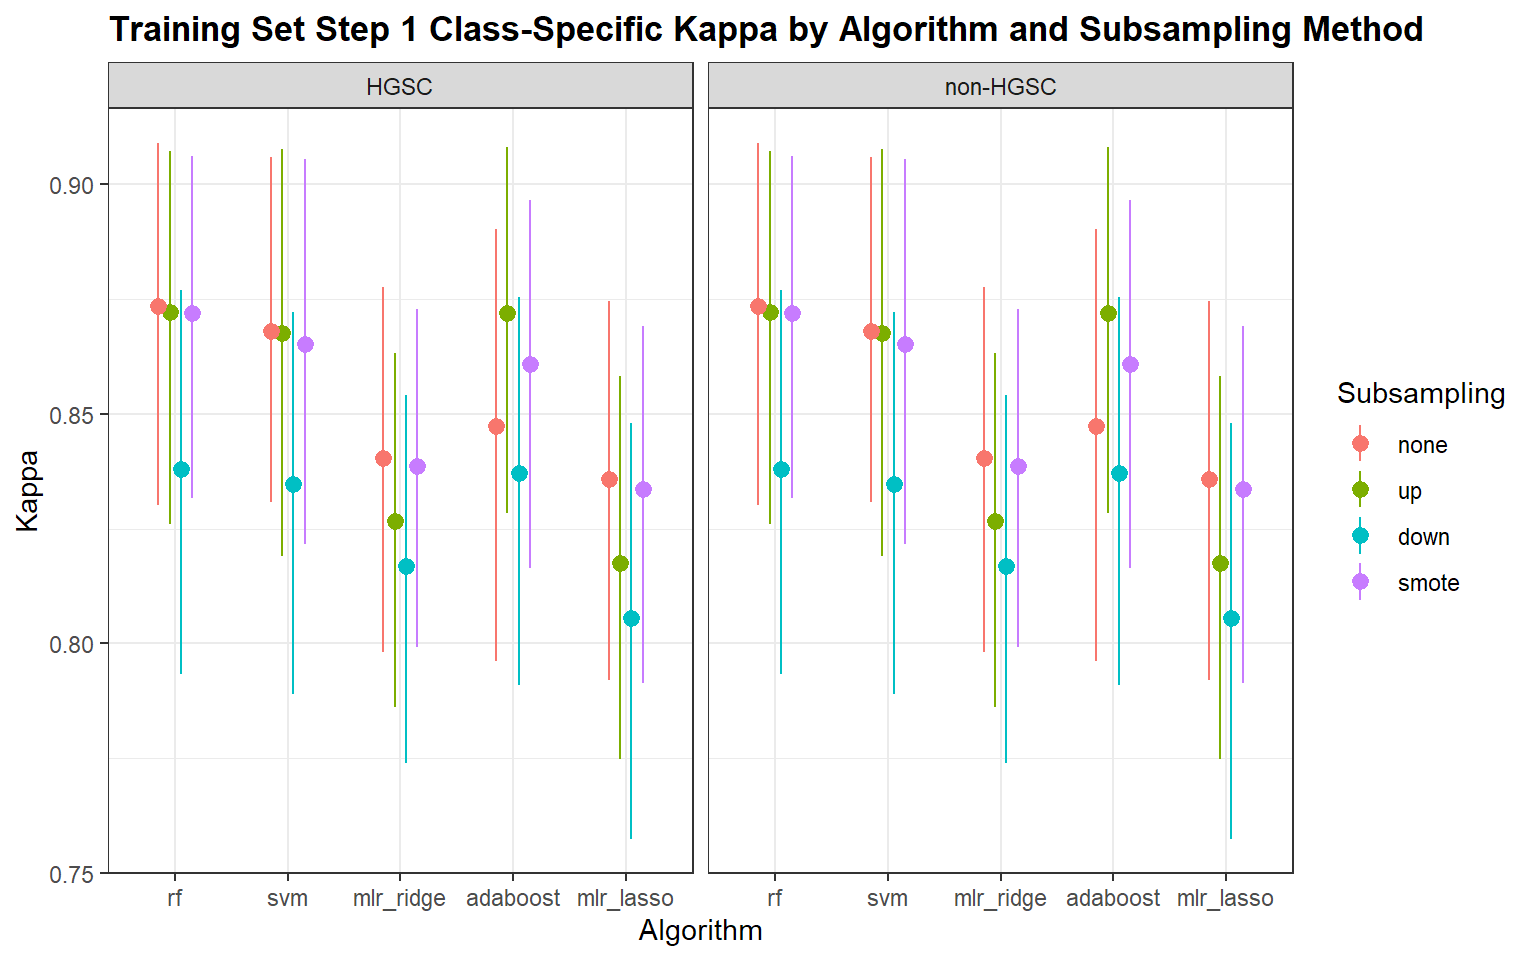
\includegraphics{OV_Histotypes_RSF_files/figure-latex/train-step1-kappa-class-1} 

}

\caption{Training Set Step 1 Class-Specific Kappa}\label{fig:train-step1-kappa-class}
\end{figure}

\begin{figure}[H]

{\centering 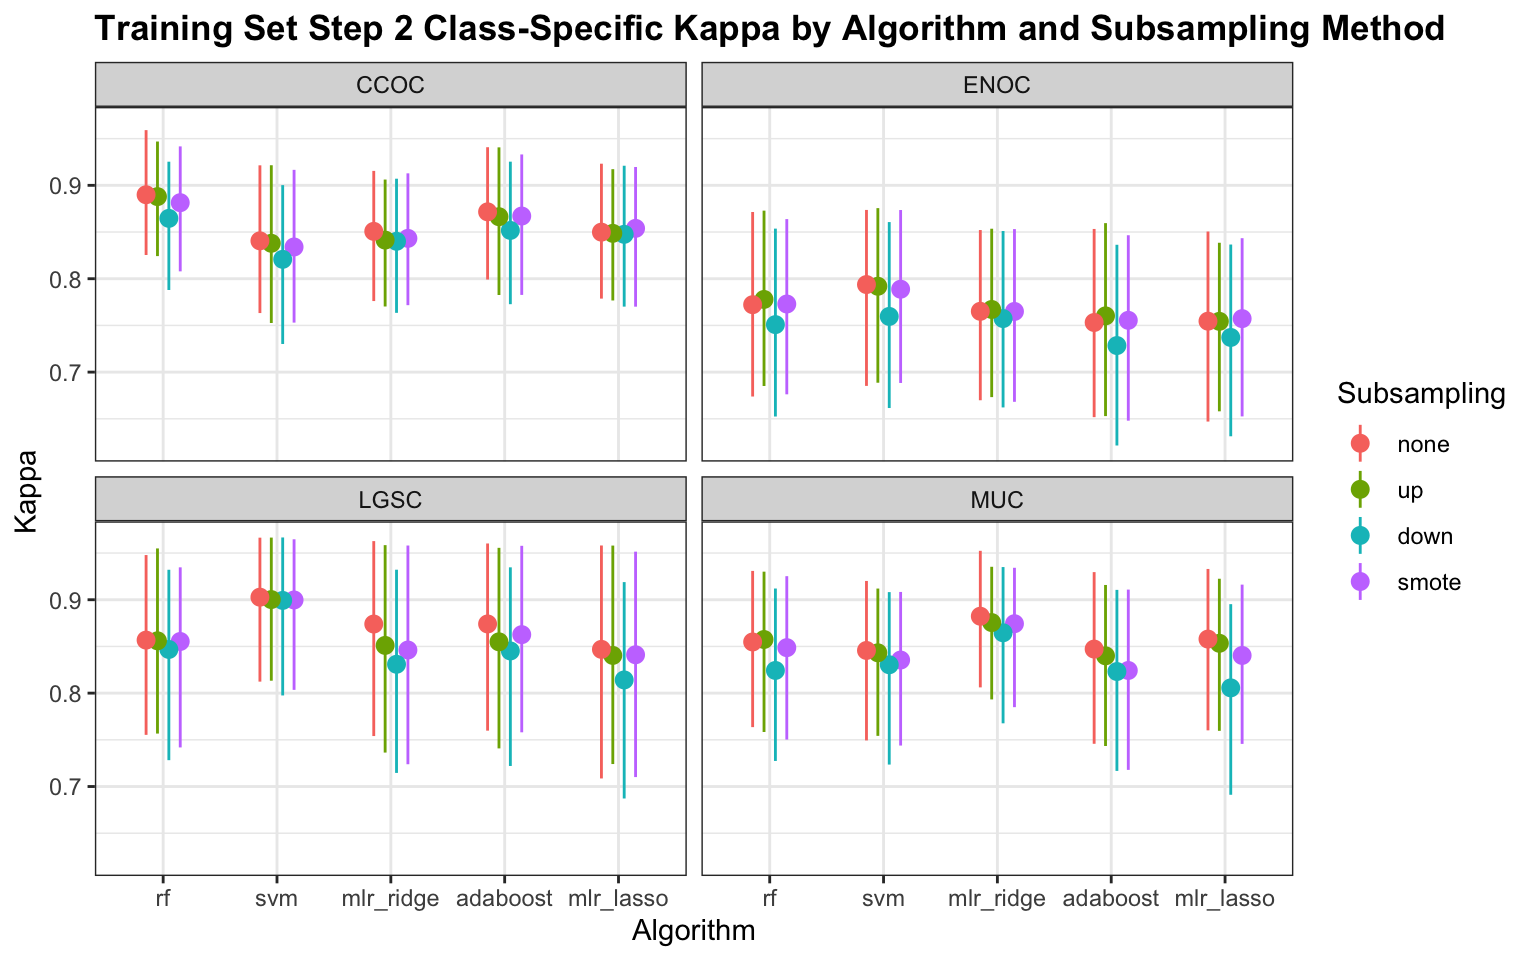
\includegraphics{OV_Histotypes_RSF_files/figure-latex/train-step2-kappa-class-1} 

}

\caption{Training Set Step 2 Class-Specific Kappa}\label{fig:train-step2-kappa-class}
\end{figure}

\begin{table}

\caption{\label{tab:train-step1-kappa-class-table}Training Set Step 1 Class-Specific Kappa by Algorithm and Subsampling Method}
\centering
\begin{tabular}[t]{l|l|l|l|l|l|l}
\hline
sampling & histotype & rf & svm & mlr\_ridge & adaboost & mlr\_lasso\\
\hline
none & HGSC & \textbf{0.865} & 0.861 & 0.83 & 0.842 & 0.826\\
\hline
none & non-HGSC & \textbf{0.865} & 0.861 & 0.83 & 0.842 & 0.826\\
\hline
up & HGSC & 0.863 & 0.862 & 0.82 & 0.859 & 0.809\\
\hline
up & non-HGSC & 0.863 & 0.862 & 0.82 & 0.859 & 0.809\\
\hline
down & HGSC & 0.827 & 0.821 & 0.809 & 0.831 & 0.791\\
\hline
down & non-HGSC & 0.827 & 0.821 & 0.809 & 0.831 & 0.791\\
\hline
smote & HGSC & 0.864 & 0.858 & 0.829 & 0.851 & 0.824\\
\hline
smote & non-HGSC & 0.864 & 0.858 & 0.829 & 0.851 & 0.824\\
\hline
\end{tabular}
\end{table}

\begin{table}

\caption{\label{tab:train-step2-kappa-class-table}Training Set Step 2 Class-Specific Kappa by Algorithm and Subsampling Method}
\centering
\begin{tabular}[t]{l|l|l|l|l|l|l}
\hline
sampling & histotype & rf & svm & mlr\_ridge & adaboost & mlr\_lasso\\
\hline
none & CCOC & 0.882 & 0.837 & 0.855 & 0.868 & 0.849\\
\hline
none & ENOC & 0.76 & 0.784 & 0.765 & 0.743 & 0.75\\
\hline
none & LGSC & 0.862 & \textbf{0.907} & 0.868 & 0.865 & 0.84\\
\hline
none & MUC & 0.849 & 0.836 & 0.87 & 0.821 & 0.844\\
\hline
up & CCOC & 0.88 & 0.834 & 0.85 & 0.859 & 0.845\\
\hline
up & ENOC & 0.763 & 0.785 & 0.766 & 0.748 & 0.749\\
\hline
up & LGSC & 0.856 & 0.905 & 0.846 & 0.862 & 0.839\\
\hline
up & MUC & 0.851 & 0.832 & 0.863 & 0.832 & 0.837\\
\hline
down & CCOC & 0.86 & 0.815 & 0.842 & 0.849 & 0.844\\
\hline
down & ENOC & 0.738 & 0.753 & 0.755 & 0.726 & 0.739\\
\hline
down & LGSC & 0.848 & 0.894 & 0.824 & 0.854 & 0.814\\
\hline
down & MUC & 0.834 & 0.814 & 0.85 & 0.819 & 0.81\\
\hline
smote & CCOC & 0.871 & 0.831 & 0.849 & 0.855 & 0.848\\
\hline
smote & ENOC & 0.763 & 0.781 & 0.766 & 0.745 & 0.751\\
\hline
smote & LGSC & 0.857 & 0.899 & 0.837 & 0.866 & 0.837\\
\hline
smote & MUC & 0.852 & 0.831 & 0.862 & 0.825 & 0.832\\
\hline
\end{tabular}
\end{table}

\hypertarget{g-mean-1}{%
\subsection{G-mean}\label{g-mean-1}}

\begin{figure}[H]

{\centering 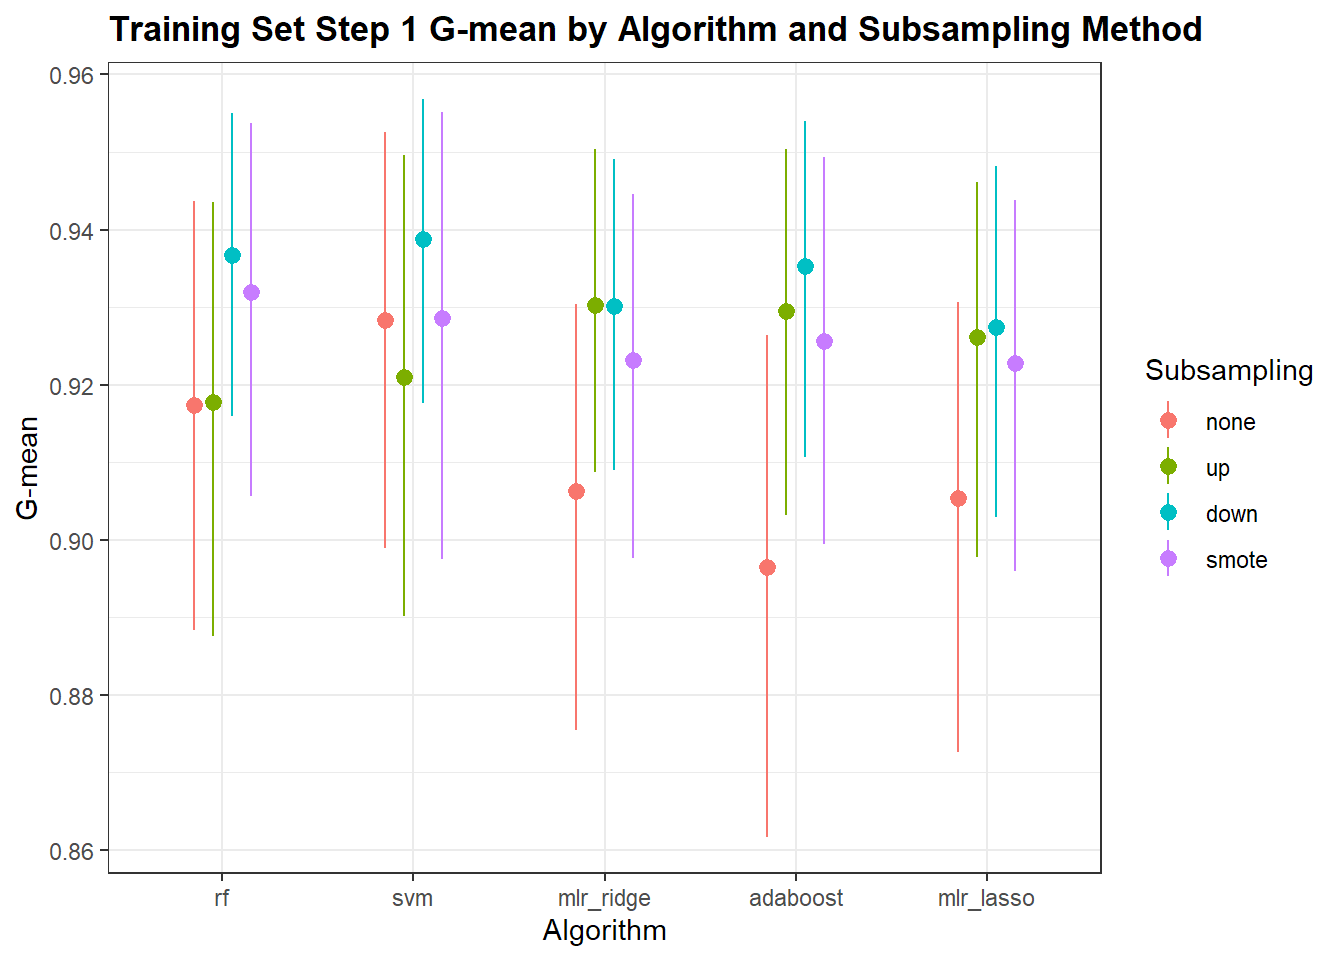
\includegraphics{OV_Histotypes_RSF_files/figure-latex/train-step1-gmean-1} 

}

\caption{Training Set Step 1 G-mean}\label{fig:train-step1-gmean}
\end{figure}

\begin{figure}[H]

{\centering 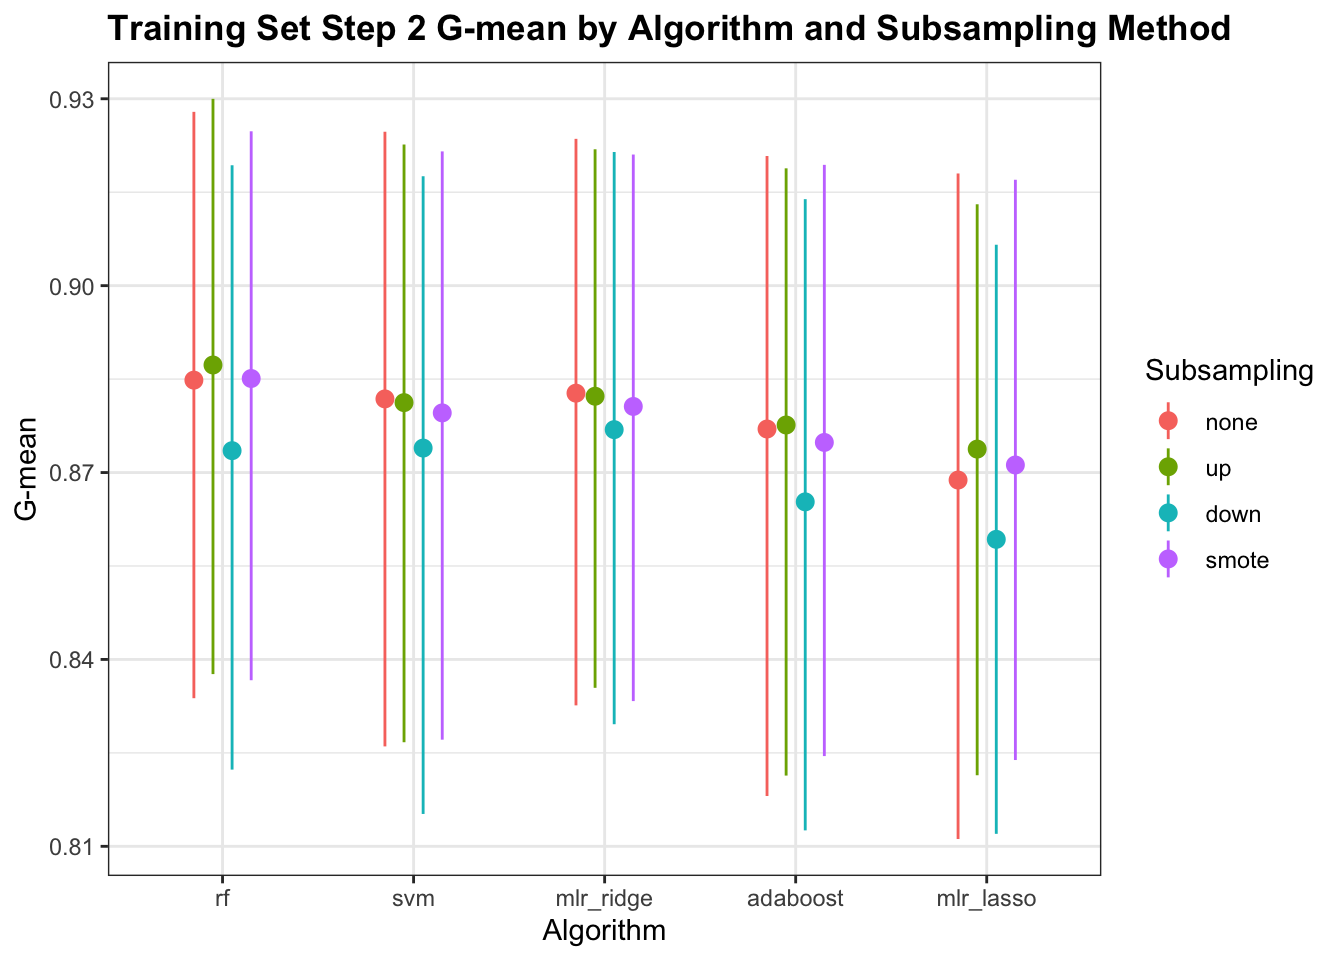
\includegraphics{OV_Histotypes_RSF_files/figure-latex/train-step2-gmean-1} 

}

\caption{Training Set Step 2 G-mean}\label{fig:train-step2-gmean}
\end{figure}

\begin{table}

\caption{\label{tab:train-step1-gmean-table}Training Set Step 1 G-mean by Algorithm and Subsampling Method}
\centering
\begin{tabular}[t]{l|l|l|l|l|l}
\hline
sampling & rf & svm & mlr\_ridge & adaboost & mlr\_lasso\\
\hline
none & 0.915 & 0.922 & 0.902 & 0.896 & 0.9\\
\hline
up & 0.914 & 0.92 & 0.929 & 0.922 & 0.924\\
\hline
down & \textbf{0.935} & \textbf{0.935} & 0.929 & 0.933 & 0.925\\
\hline
smote & 0.928 & 0.926 & 0.92 & 0.921 & 0.919\\
\hline
\end{tabular}
\end{table}

\begin{table}

\caption{\label{tab:train-step2-gmean-table}Training Set Step 2 G-mean by Algorithm and Subsampling Method}
\centering
\begin{tabular}[t]{l|l|l|l|l|l}
\hline
sampling & rf & svm & mlr\_ridge & adaboost & mlr\_lasso\\
\hline
none & 0.881 & 0.878 & 0.88 & 0.871 & 0.867\\
\hline
up & \textbf{0.884} & 0.878 & 0.88 & 0.873 & 0.868\\
\hline
down & 0.873 & 0.869 & 0.873 & 0.865 & 0.859\\
\hline
smote & 0.882 & 0.875 & 0.878 & 0.872 & 0.87\\
\hline
\end{tabular}
\end{table}

\begin{figure}[H]

{\centering 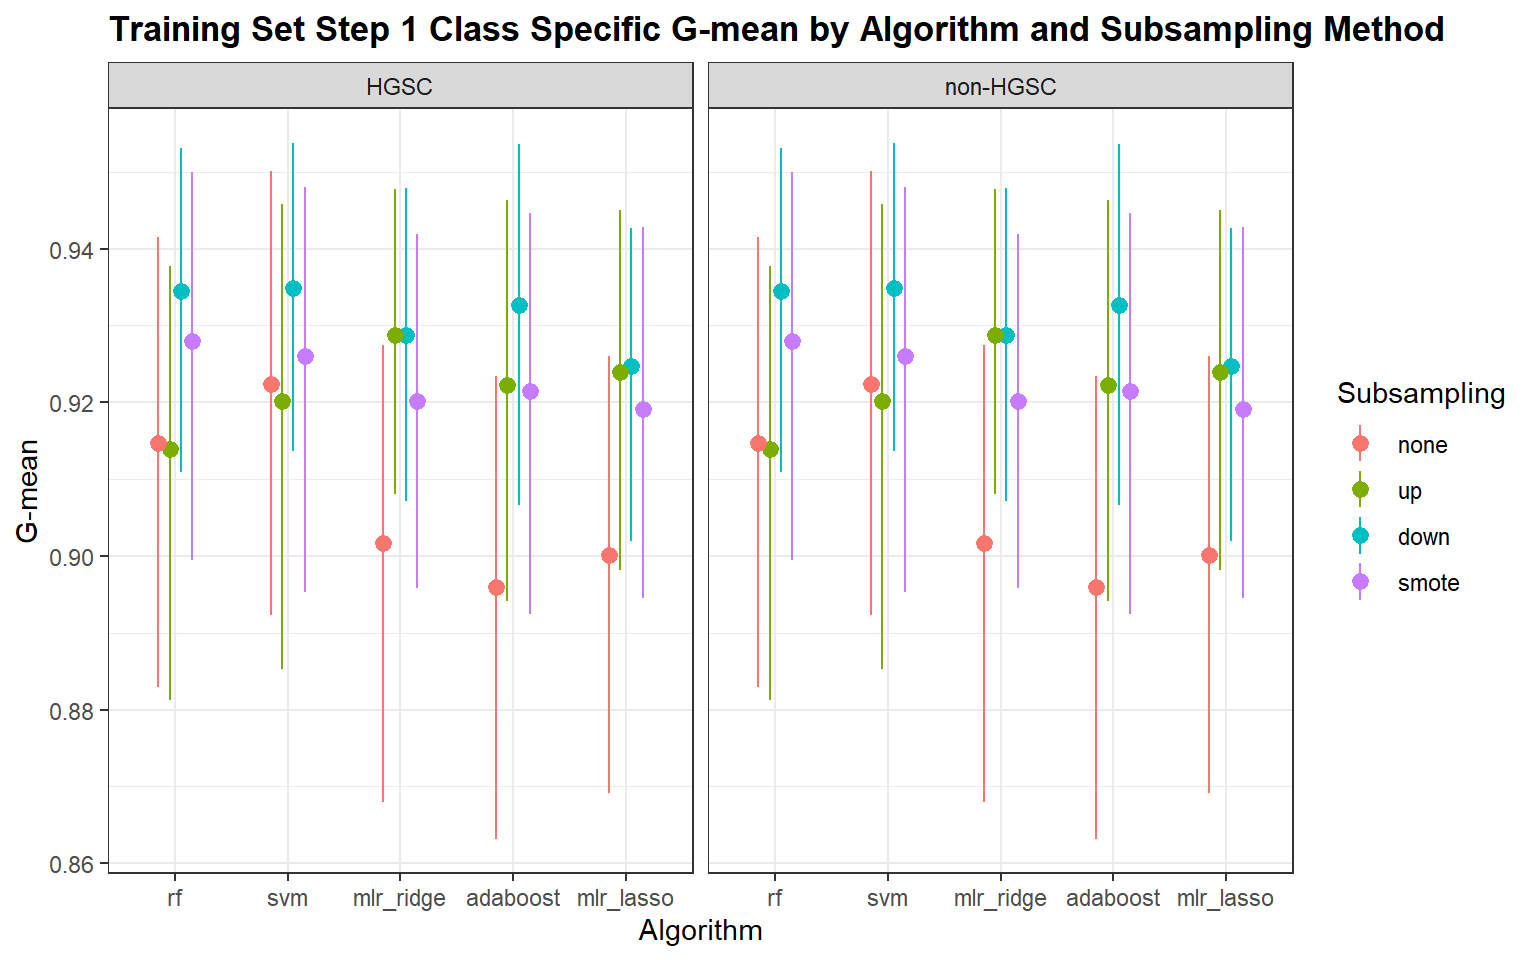
\includegraphics{OV_Histotypes_RSF_files/figure-latex/train-step1-gmean-class-1} 

}

\caption{Training Set Step 1 Class-Specific G-mean}\label{fig:train-step1-gmean-class}
\end{figure}

\begin{figure}[H]

{\centering 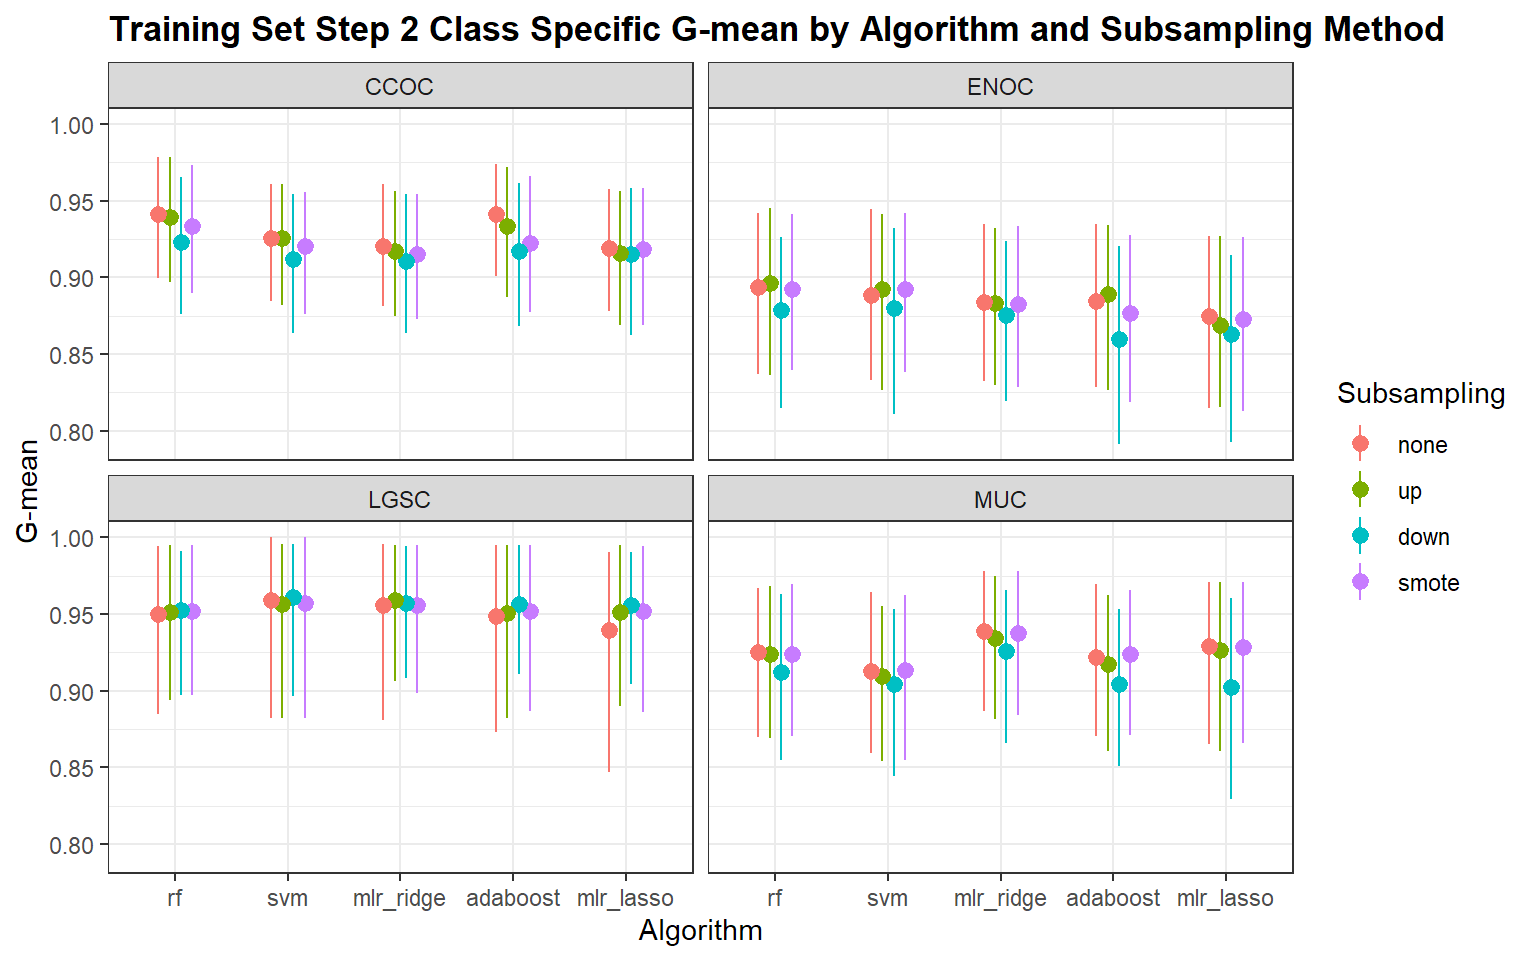
\includegraphics{OV_Histotypes_RSF_files/figure-latex/train-step2-gmean-class-1} 

}

\caption{Training Set Step 2 Class-Specific G-mean}\label{fig:train-step2-gmean-class}
\end{figure}

\begin{table}

\caption{\label{tab:train-step1-gmean-class-table}Training Set Step 1 Class-Specific G-mean by Algorithm and Subsampling Method}
\centering
\begin{tabular}[t]{l|l|l|l|l|l|l}
\hline
sampling & histotype & rf & svm & mlr\_ridge & adaboost & mlr\_lasso\\
\hline
none & HGSC & 0.915 & 0.922 & 0.902 & 0.896 & 0.9\\
\hline
none & non-HGSC & 0.915 & 0.922 & 0.902 & 0.896 & 0.9\\
\hline
up & HGSC & 0.914 & 0.92 & 0.929 & 0.922 & 0.924\\
\hline
up & non-HGSC & 0.914 & 0.92 & 0.929 & 0.922 & 0.924\\
\hline
down & HGSC & \textbf{0.935} & \textbf{0.935} & 0.929 & 0.933 & 0.925\\
\hline
down & non-HGSC & \textbf{0.935} & \textbf{0.935} & 0.929 & 0.933 & 0.925\\
\hline
smote & HGSC & 0.928 & 0.926 & 0.92 & 0.921 & 0.919\\
\hline
smote & non-HGSC & 0.928 & 0.926 & 0.92 & 0.921 & 0.919\\
\hline
\end{tabular}
\end{table}

\begin{table}

\caption{\label{tab:train-step2-gmean-class-table}Training Set Step 2 Class-Specific G-mean by Algorithm and Subsampling Method}
\centering
\begin{tabular}[t]{l|l|l|l|l|l|l}
\hline
sampling & histotype & rf & svm & mlr\_ridge & adaboost & mlr\_lasso\\
\hline
none & CCOC & 0.939 & 0.921 & 0.925 & 0.928 & 0.923\\
\hline
none & ENOC & 0.885 & 0.891 & 0.885 & 0.877 & 0.874\\
\hline
none & LGSC & 0.944 & 0.953 & 0.94 & 0.938 & 0.922\\
\hline
none & MUC & 0.918 & 0.92 & 0.933 & 0.908 & 0.924\\
\hline
up & CCOC & 0.936 & 0.92 & 0.92 & 0.921 & 0.918\\
\hline
up & ENOC & 0.889 & 0.891 & 0.885 & 0.88 & 0.871\\
\hline
up & LGSC & 0.947 & 0.951 & 0.947 & 0.942 & 0.941\\
\hline
up & MUC & 0.92 & 0.913 & 0.929 & 0.913 & 0.921\\
\hline
down & CCOC & 0.923 & 0.907 & 0.913 & 0.918 & 0.918\\
\hline
down & ENOC & 0.871 & 0.877 & 0.879 & 0.859 & 0.867\\
\hline
down & LGSC & 0.951 & \textbf{0.957} & 0.948 & 0.954 & 0.946\\
\hline
down & MUC & 0.912 & 0.904 & 0.92 & 0.913 & 0.901\\
\hline
smote & CCOC & 0.929 & 0.914 & 0.917 & 0.918 & 0.92\\
\hline
smote & ENOC & 0.888 & 0.895 & 0.887 & 0.877 & 0.873\\
\hline
smote & LGSC & 0.951 & 0.951 & 0.946 & 0.951 & 0.945\\
\hline
smote & MUC & 0.919 & 0.916 & 0.928 & 0.913 & 0.918\\
\hline
\end{tabular}
\end{table}

\hypertarget{cs1-set}{%
\section{CS1 Set}\label{cs1-set}}

\hypertarget{accuracy-2}{%
\subsection{Accuracy}\label{accuracy-2}}

\begin{figure}[H]

{\centering 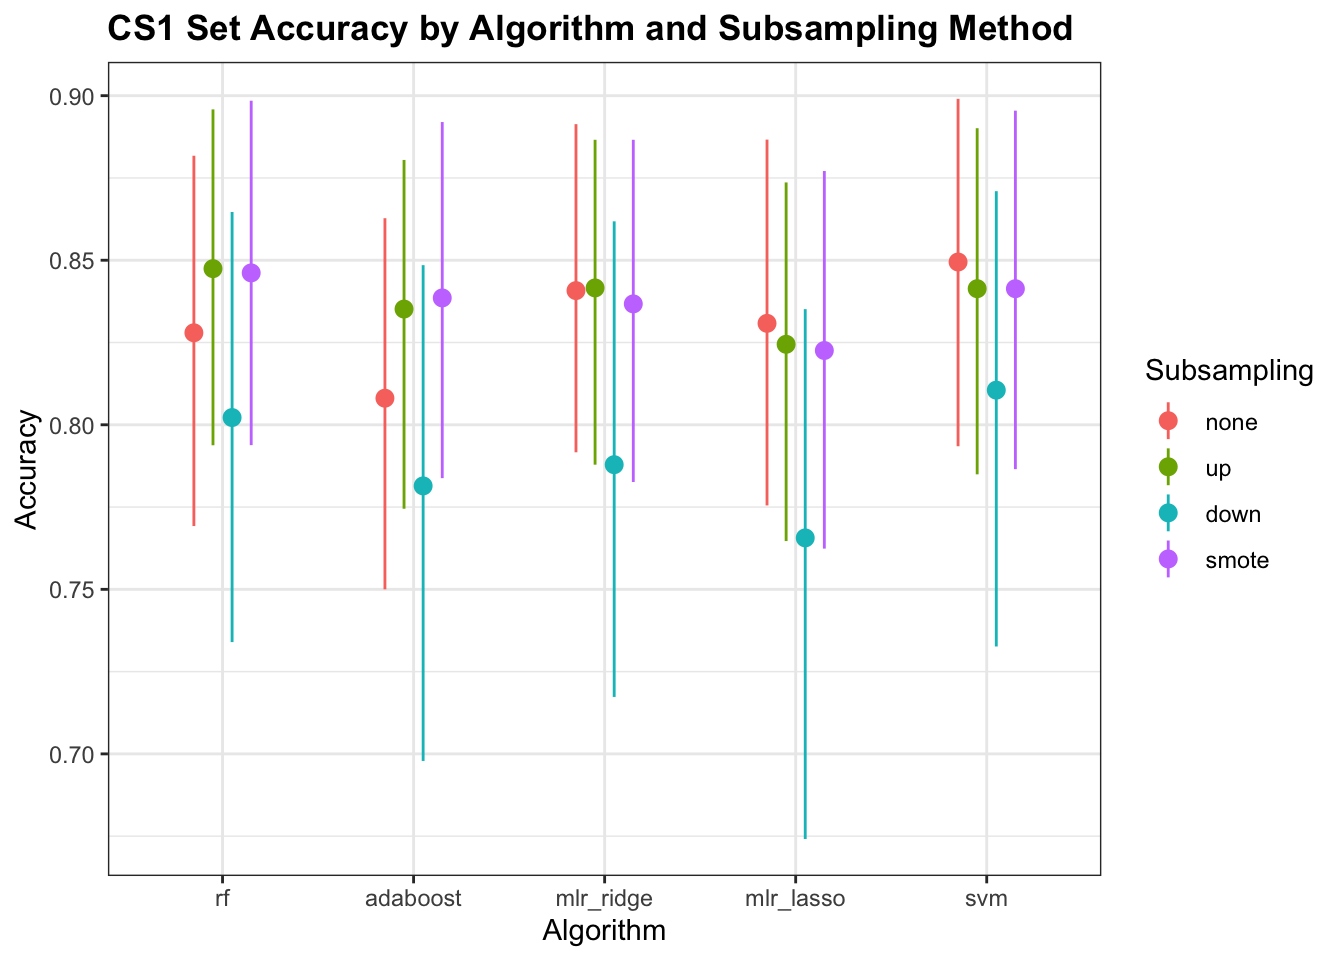
\includegraphics{OV_Histotypes_RSF_files/figure-latex/cs1-accuracy-1} 

}

\caption{CS1 Set Accuracy}\label{fig:cs1-accuracy}
\end{figure}

\begin{table}

\caption{\label{tab:cs1-accuracy-table}CS1 Set Accuracy by Algorithm and Subsampling Method}
\centering
\begin{tabular}[t]{l|l|l|l|l|l}
\hline
sampling & rf & svm & mlr\_ridge & adaboost & mlr\_lasso\\
\hline
none & 0.816 & \textbf{0.842} & 0.832 & 0.8 & 0.823\\
\hline
up & 0.835 & 0.833 & 0.83 & 0.825 & 0.814\\
\hline
down & 0.798 & 0.802 & 0.788 & 0.776 & 0.764\\
\hline
smote & 0.837 & 0.837 & 0.83 & 0.828 & 0.814\\
\hline
\end{tabular}
\end{table}

\begin{figure}[H]

{\centering 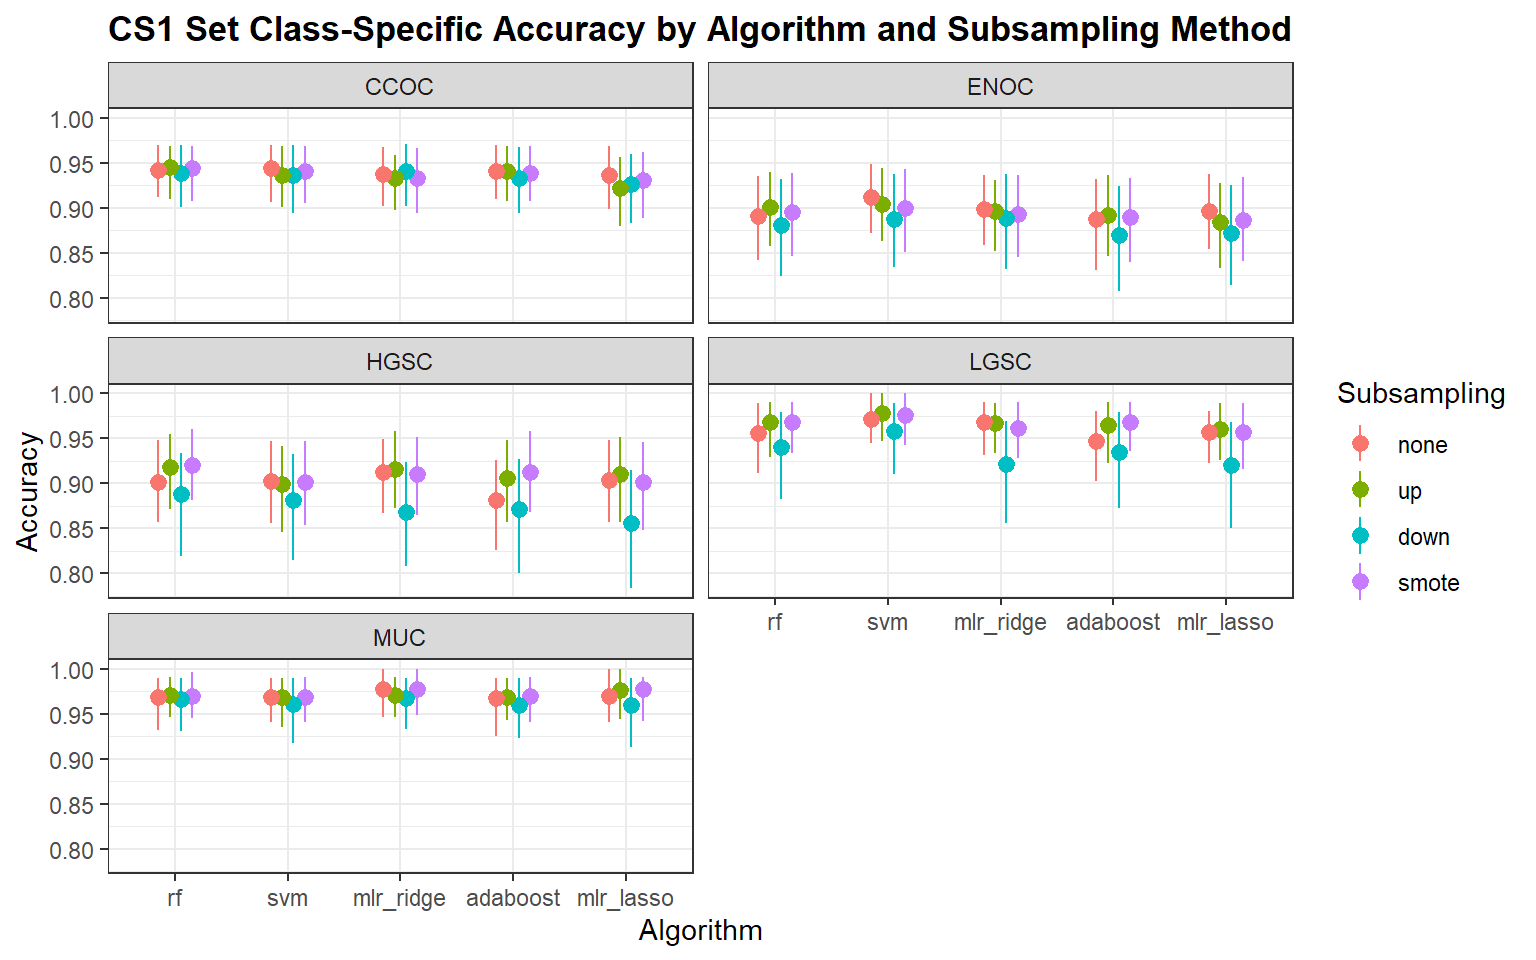
\includegraphics{OV_Histotypes_RSF_files/figure-latex/cs1-accuracy-class-1} 

}

\caption{CS1 Set Class-Specific Accuracy}\label{fig:cs1-accuracy-class}
\end{figure}

\begin{table}

\caption{\label{tab:cs1-accuracy-class-table}CS1 Set Class-Specific Accuracy by Algorithm and Subsampling Method}
\centering
\begin{tabular}[t]{l|l|l|l|l|l|l}
\hline
sampling & histotype & rf & svm & mlr\_ridge & adaboost & mlr\_lasso\\
\hline
none & CCOC & 0.939 & 0.943 & 0.935 & 0.939 & 0.931\\
\hline
none & ENOC & 0.894 & 0.917 & 0.902 & 0.892 & 0.9\\
\hline
none & HGSC & 0.891 & 0.894 & 0.903 & 0.87 & 0.896\\
\hline
none & LGSC & 0.95 & 0.969 & 0.96 & 0.943 & 0.957\\
\hline
none & MUC & 0.966 & 0.962 & 0.969 & 0.96 & 0.969\\
\hline
up & CCOC & 0.942 & 0.938 & 0.927 & 0.939 & 0.918\\
\hline
up & ENOC & 0.902 & 0.906 & 0.899 & 0.897 & 0.885\\
\hline
up & HGSC & 0.907 & 0.894 & 0.908 & 0.897 & 0.903\\
\hline
up & LGSC & 0.96 & \textbf{0.971} & 0.959 & 0.958 & 0.958\\
\hline
up & MUC & 0.967 & 0.963 & 0.968 & 0.961 & 0.969\\
\hline
down & CCOC & 0.936 & 0.938 & 0.937 & 0.932 & 0.922\\
\hline
down & ENOC & 0.887 & 0.895 & 0.892 & 0.876 & 0.878\\
\hline
down & HGSC & 0.883 & 0.874 & 0.872 & 0.869 & 0.858\\
\hline
down & LGSC & 0.939 & 0.949 & 0.925 & 0.935 & 0.921\\
\hline
down & MUC & 0.958 & 0.954 & 0.96 & 0.95 & 0.957\\
\hline
smote & CCOC & 0.94 & 0.939 & 0.929 & 0.939 & 0.926\\
\hline
smote & ENOC & 0.892 & 0.905 & 0.896 & 0.888 & 0.891\\
\hline
smote & HGSC & 0.916 & 0.897 & 0.907 & 0.905 & 0.894\\
\hline
smote & LGSC & 0.961 & 0.97 & 0.96 & 0.963 & 0.957\\
\hline
smote & MUC & 0.962 & 0.967 & 0.968 & 0.96 & 0.969\\
\hline
\end{tabular}
\end{table}

\hypertarget{f1-score-2}{%
\subsection{F1-Score}\label{f1-score-2}}

\begin{figure}[H]

{\centering 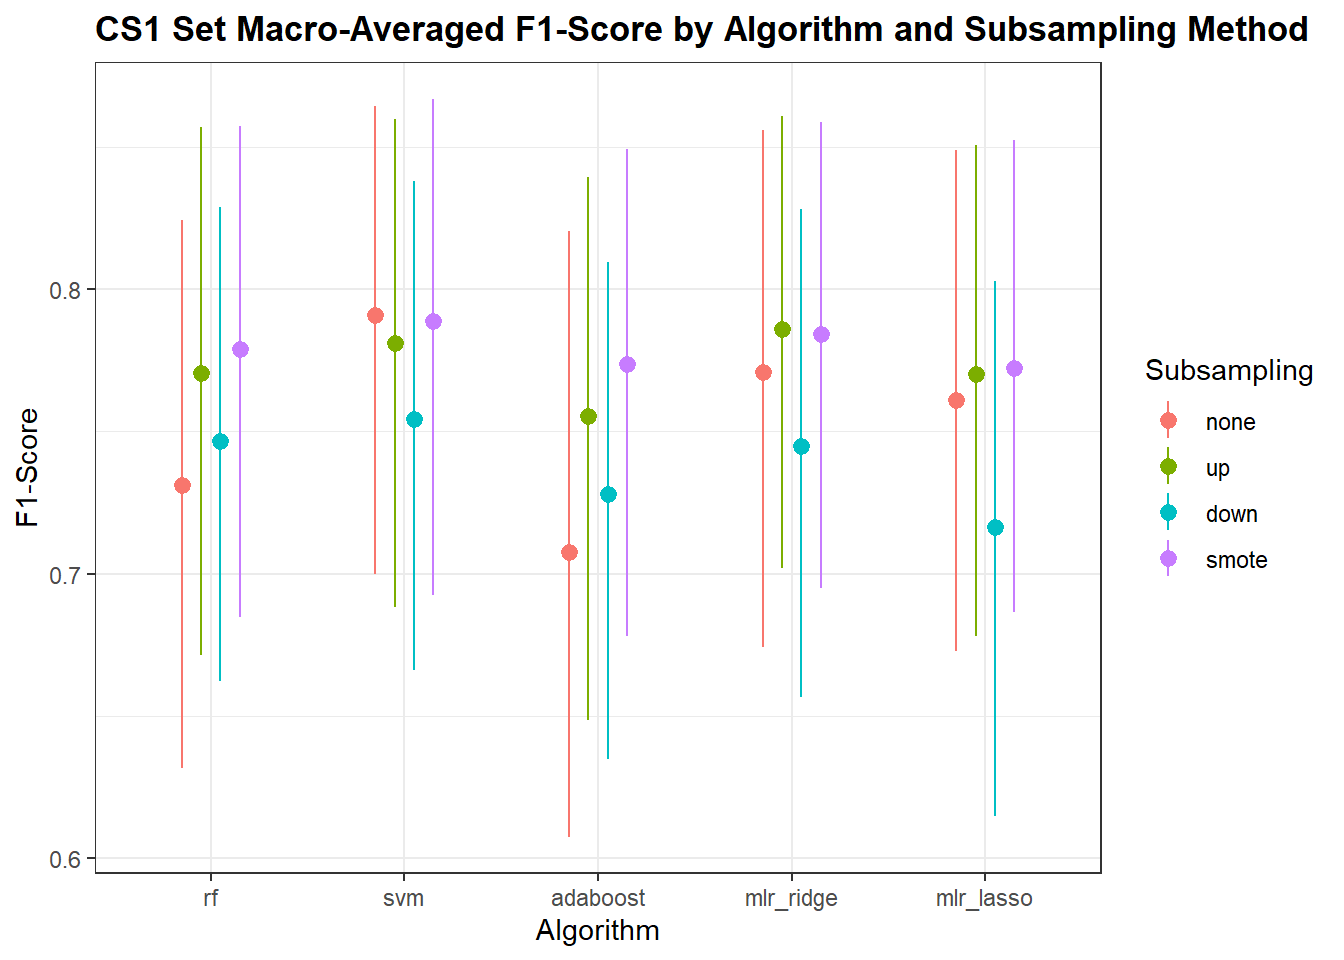
\includegraphics{OV_Histotypes_RSF_files/figure-latex/cs1-f1-1} 

}

\caption{CS1 Set F1-Score}\label{fig:cs1-f1}
\end{figure}

\begin{table}

\caption{\label{tab:cs1-f1-table}CS1 Set Macro-Averaged F1-Score by Algorithm and Subsampling Method}
\centering
\begin{tabular}[t]{l|l|l|l|l|l}
\hline
sampling & rf & svm & mlr\_ridge & adaboost & mlr\_lasso\\
\hline
none & 0.731 & \textbf{0.791} & 0.771 & 0.707 & 0.761\\
\hline
up & 0.77 & 0.781 & 0.786 & 0.755 & 0.77\\
\hline
down & 0.746 & 0.754 & 0.745 & 0.728 & 0.716\\
\hline
smote & 0.779 & 0.789 & 0.784 & 0.773 & 0.773\\
\hline
\end{tabular}
\end{table}

\begin{figure}[H]

{\centering 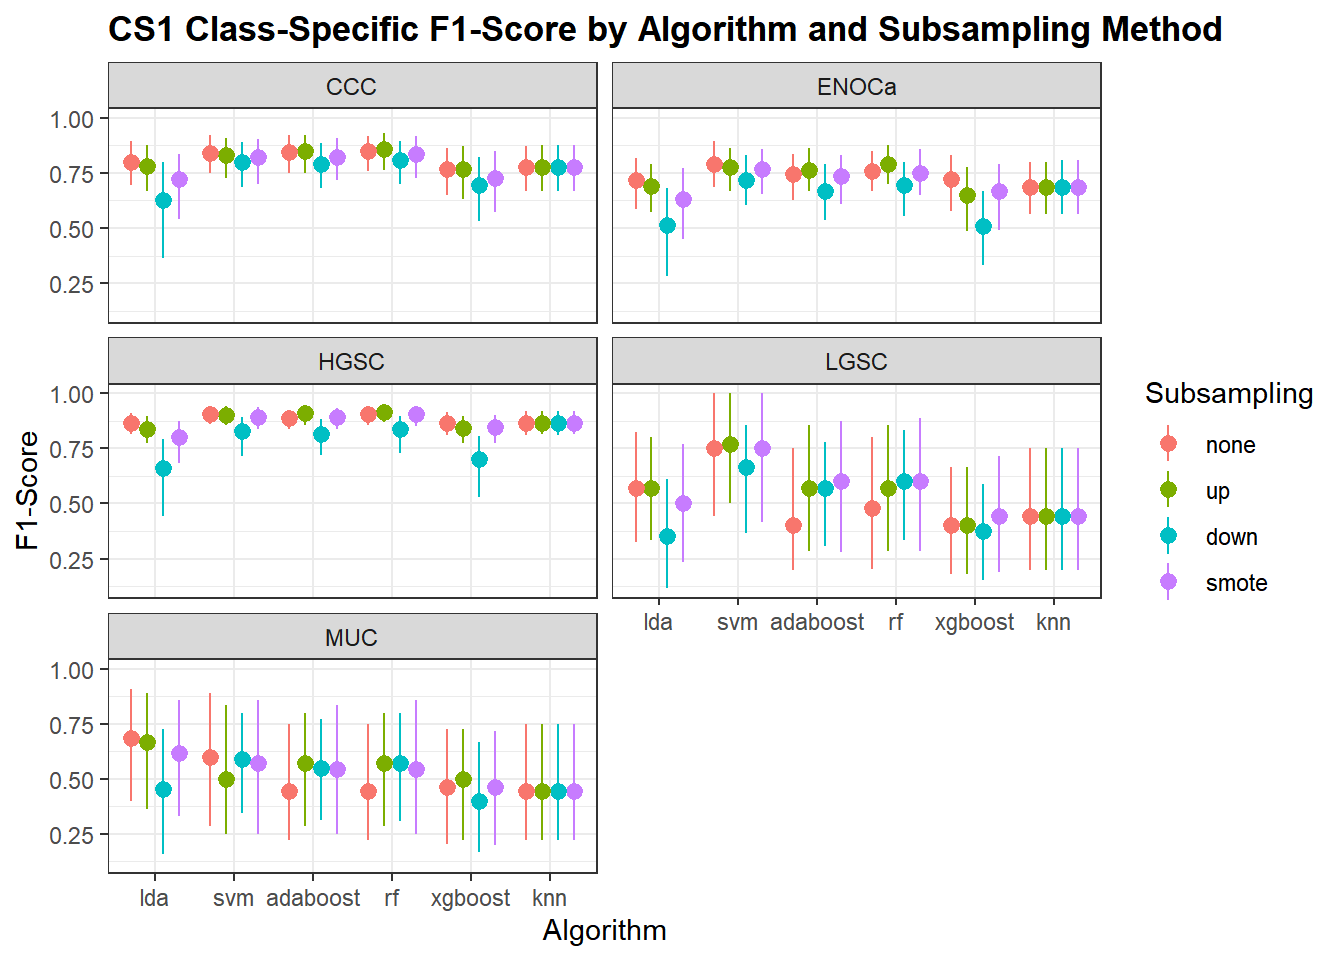
\includegraphics{OV_Histotypes_RSF_files/figure-latex/cs1-f1-class-1} 

}

\caption{CS1 Set Class-Specific F1-Score}\label{fig:cs1-f1-class}
\end{figure}

\begin{table}

\caption{\label{tab:cs1-f1-class-table}CS1 Set Class-Specific F1-Score by Algorithm and Subsampling Method}
\centering
\begin{tabular}[t]{l|l|l|l|l|l|l}
\hline
sampling & histotype & rf & svm & mlr\_ridge & adaboost & mlr\_lasso\\
\hline
none & CCOC & 0.824 & 0.828 & 0.812 & 0.824 & 0.8\\
\hline
none & ENOC & 0.762 & 0.8 & 0.769 & 0.745 & 0.772\\
\hline
none & HGSC & 0.889 & 0.893 & 0.9 & 0.873 & 0.891\\
\hline
none & LGSC & 0.5 & 0.75 & 0.667 & 0.4 & 0.615\\
\hline
none & MUC & 0.667 & 0.714 & 0.75 & 0.667 & 0.75\\
\hline
up & CCOC & 0.833 & 0.815 & 0.8 & 0.824 & 0.773\\
\hline
up & ENOC & 0.78 & 0.783 & 0.769 & 0.765 & 0.744\\
\hline
up & HGSC & 0.905 & 0.893 & 0.901 & 0.895 & 0.891\\
\hline
up & LGSC & 0.667 & 0.769 & 0.727 & 0.615 & 0.714\\
\hline
up & MUC & 0.727 & 0.667 & 0.75 & 0.714 & 0.762\\
\hline
down & CCOC & 0.822 & 0.824 & 0.821 & 0.811 & 0.786\\
\hline
down & ENOC & 0.75 & 0.769 & 0.762 & 0.718 & 0.723\\
\hline
down & HGSC & 0.864 & 0.857 & 0.851 & 0.85 & 0.835\\
\hline
down & LGSC & 0.632 & 0.667 & 0.588 & 0.615 & 0.571\\
\hline
down & MUC & 0.706 & 0.706 & 0.714 & 0.667 & 0.667\\
\hline
smote & CCOC & 0.829 & 0.828 & 0.81 & 0.828 & 0.789\\
\hline
smote & ENOC & 0.769 & 0.783 & 0.766 & 0.756 & 0.757\\
\hline
smote & HGSC & \textbf{0.909} & 0.892 & 0.897 & 0.899 & 0.884\\
\hline
smote & LGSC & 0.714 & 0.75 & 0.727 & 0.714 & 0.706\\
\hline
smote & MUC & 0.727 & 0.714 & 0.75 & 0.706 & 0.762\\
\hline
\end{tabular}
\end{table}

\hypertarget{kappa-2}{%
\subsection{Kappa}\label{kappa-2}}

\begin{figure}[H]

{\centering 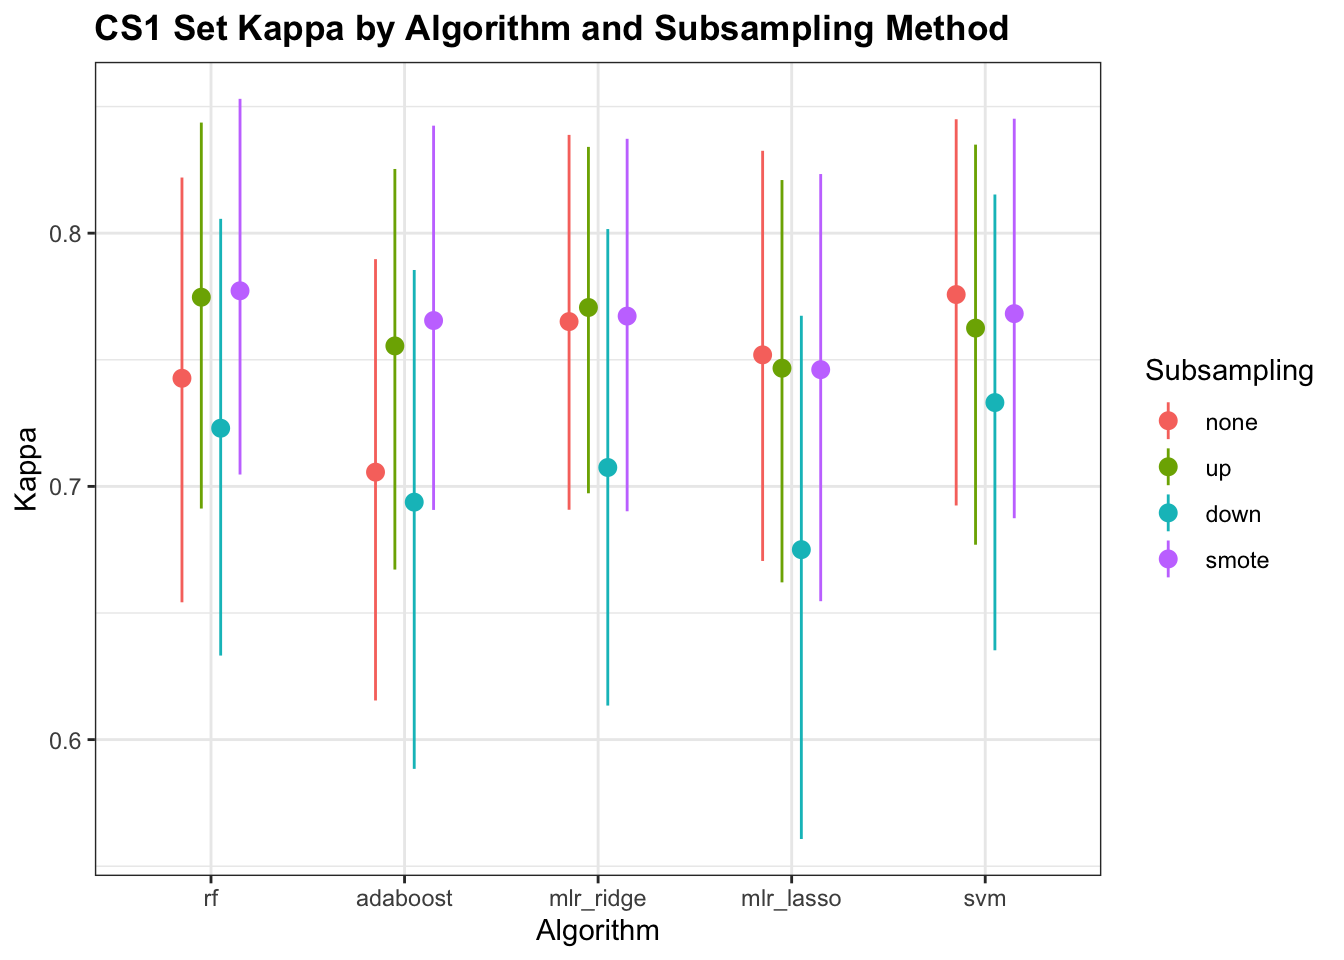
\includegraphics{OV_Histotypes_RSF_files/figure-latex/cs1-kappa-1} 

}

\caption{CS1 Set Kappa}\label{fig:cs1-kappa}
\end{figure}

\begin{table}

\caption{\label{tab:cs1-kappa-table}CS1 Set Kappa by Algorithm and Subsampling Method}
\centering
\begin{tabular}[t]{l|l|l|l|l|l}
\hline
sampling & rf & svm & mlr\_ridge & adaboost & mlr\_lasso\\
\hline
none & 0.724 & \textbf{0.767} & 0.752 & 0.697 & 0.74\\
\hline
up & 0.756 & 0.752 & 0.757 & 0.741 & 0.732\\
\hline
down & 0.716 & 0.72 & 0.706 & 0.687 & 0.673\\
\hline
smote & 0.763 & 0.759 & 0.755 & 0.751 & 0.736\\
\hline
\end{tabular}
\end{table}

\begin{figure}[H]

{\centering 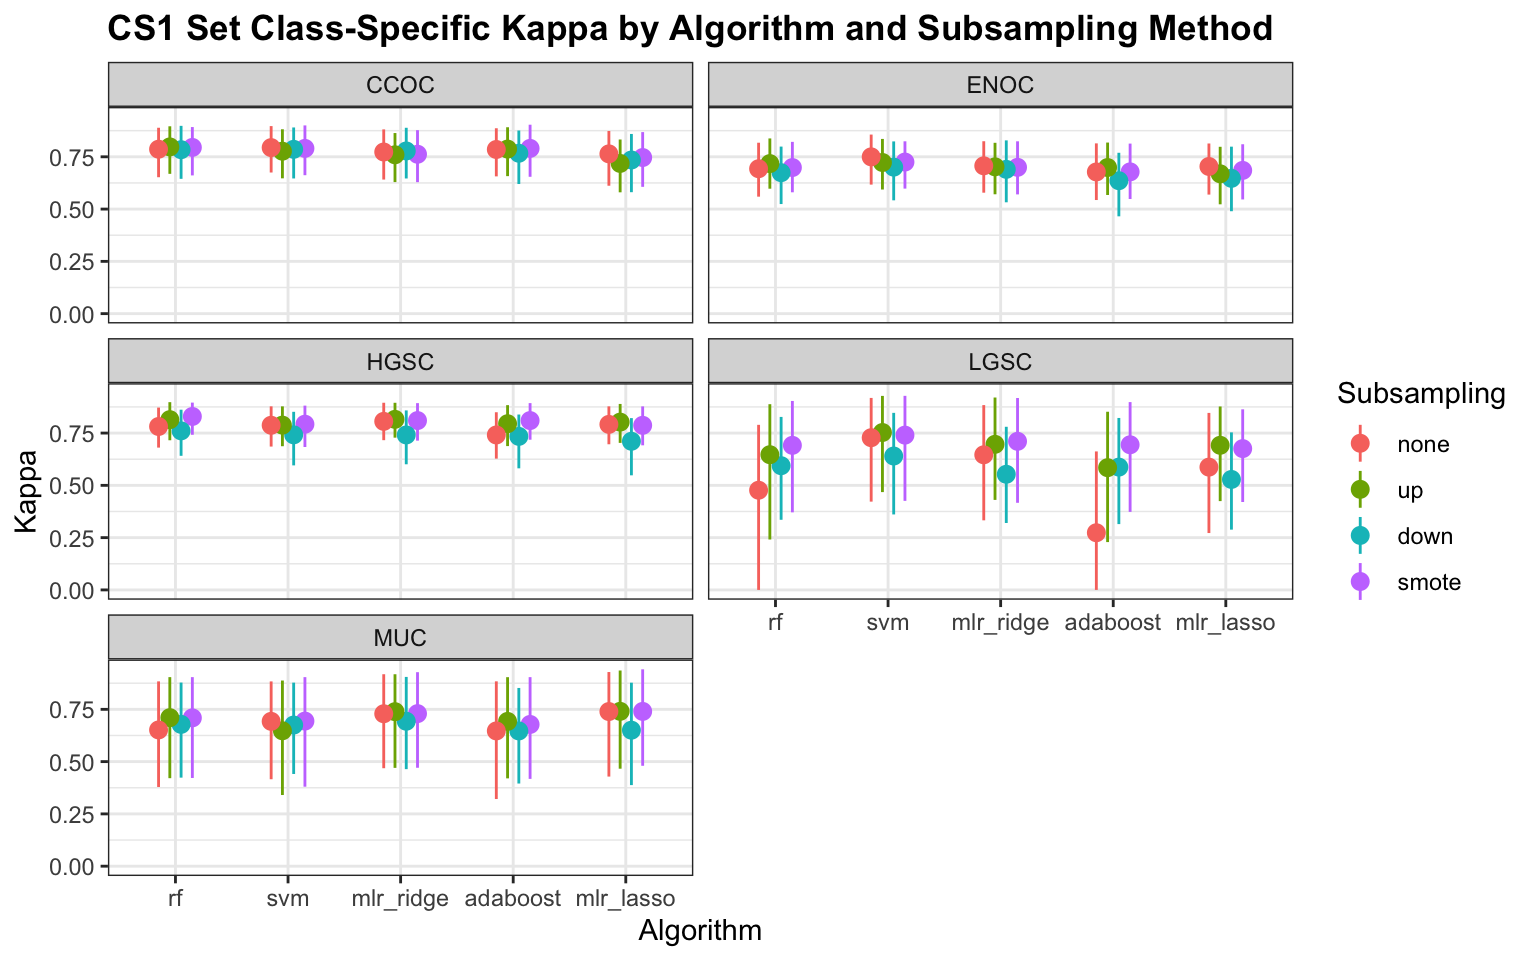
\includegraphics{OV_Histotypes_RSF_files/figure-latex/cs1-kappa-class-1} 

}

\caption{CS1 Set Class-Specific Kappa}\label{fig:cs1-kappa-class}
\end{figure}

\begin{table}

\caption{\label{tab:cs1-kappa-class-table}CS1 Set Class-Specific Kappa by Algorithm and Subsampling Method}
\centering
\begin{tabular}[t]{l|l|l|l|l|l|l}
\hline
sampling & histotype & rf & svm & mlr\_ridge & adaboost & mlr\_lasso\\
\hline
none & CCOC & 0.786 & 0.794 & 0.773 & 0.785 & 0.764\\
\hline
none & ENOC & 0.693 & 0.75 & 0.707 & 0.678 & 0.704\\
\hline
none & HGSC & 0.781 & 0.787 & 0.806 & 0.741 & 0.792\\
\hline
none & LGSC & 0.477 & 0.728 & 0.646 & 0.273 & 0.587\\
\hline
none & MUC & 0.652 & 0.693 & 0.729 & 0.647 & 0.739\\
\hline
up & CCOC & 0.797 & 0.777 & 0.76 & 0.787 & 0.718\\
\hline
up & ENOC & 0.718 & 0.723 & 0.702 & 0.699 & 0.669\\
\hline
up & HGSC & 0.814 & 0.788 & 0.816 & 0.795 & 0.802\\
\hline
up & LGSC & 0.647 & 0.753 & 0.696 & 0.585 & 0.692\\
\hline
up & MUC & 0.71 & 0.647 & 0.739 & 0.692 & 0.74\\
\hline
down & CCOC & 0.784 & 0.786 & 0.778 & 0.767 & 0.735\\
\hline
down & ENOC & 0.674 & 0.701 & 0.69 & 0.636 & 0.647\\
\hline
down & HGSC & 0.761 & 0.742 & 0.741 & 0.734 & 0.711\\
\hline
down & LGSC & 0.594 & 0.64 & 0.553 & 0.587 & 0.528\\
\hline
down & MUC & 0.678 & 0.675 & 0.693 & 0.647 & 0.65\\
\hline
smote & CCOC & 0.795 & 0.79 & 0.762 & 0.79 & 0.747\\
\hline
smote & ENOC & 0.699 & 0.725 & 0.7 & 0.678 & 0.685\\
\hline
smote & HGSC & \textbf{0.829} & 0.792 & 0.81 & 0.81 & 0.787\\
\hline
smote & LGSC & 0.691 & 0.74 & 0.711 & 0.694 & 0.676\\
\hline
smote & MUC & 0.709 & 0.694 & 0.73 & 0.678 & 0.74\\
\hline
\end{tabular}
\end{table}

\hypertarget{g-mean-2}{%
\subsection{G-mean}\label{g-mean-2}}

\begin{figure}[H]

{\centering 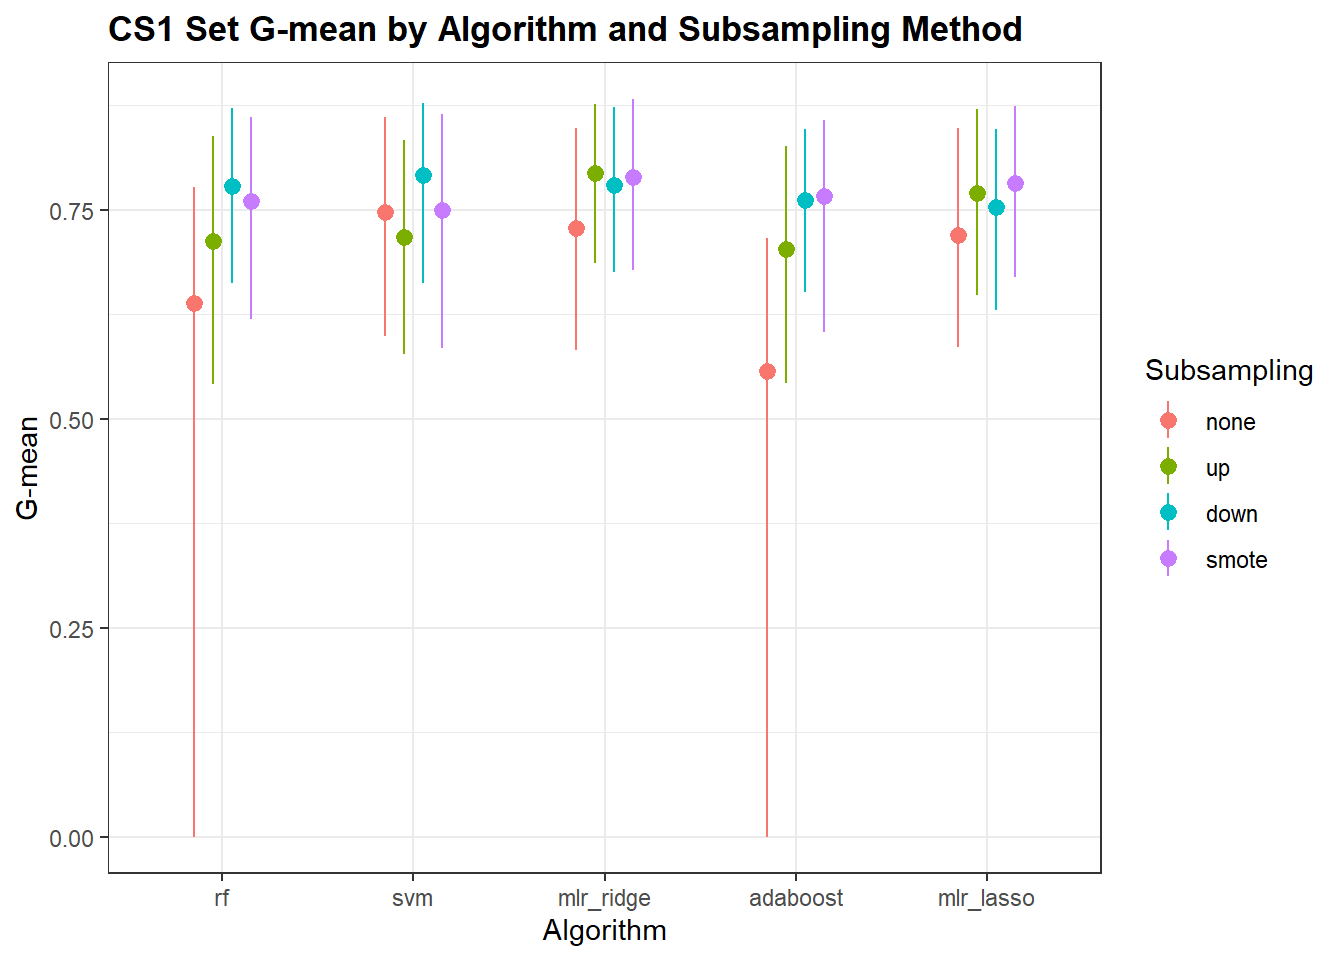
\includegraphics{OV_Histotypes_RSF_files/figure-latex/cs1-gmean-1} 

}

\caption{CS1 Set G-mean}\label{fig:cs1-gmean}
\end{figure}

\begin{table}

\caption{\label{tab:cs1-gmean-table}CS1 Set G-mean by Algorithm and Subsampling Method}
\centering
\begin{tabular}[t]{l|l|l|l|l|l}
\hline
sampling & rf & svm & mlr\_ridge & adaboost & mlr\_lasso\\
\hline
none & 0.638 & 0.747 & 0.728 & 0.557 & 0.72\\
\hline
up & 0.713 & 0.718 & \textbf{0.794} & 0.703 & 0.769\\
\hline
down & 0.778 & 0.791 & 0.779 & 0.761 & 0.753\\
\hline
smote & 0.76 & 0.75 & 0.789 & 0.766 & 0.782\\
\hline
\end{tabular}
\end{table}

\begin{figure}[H]

{\centering 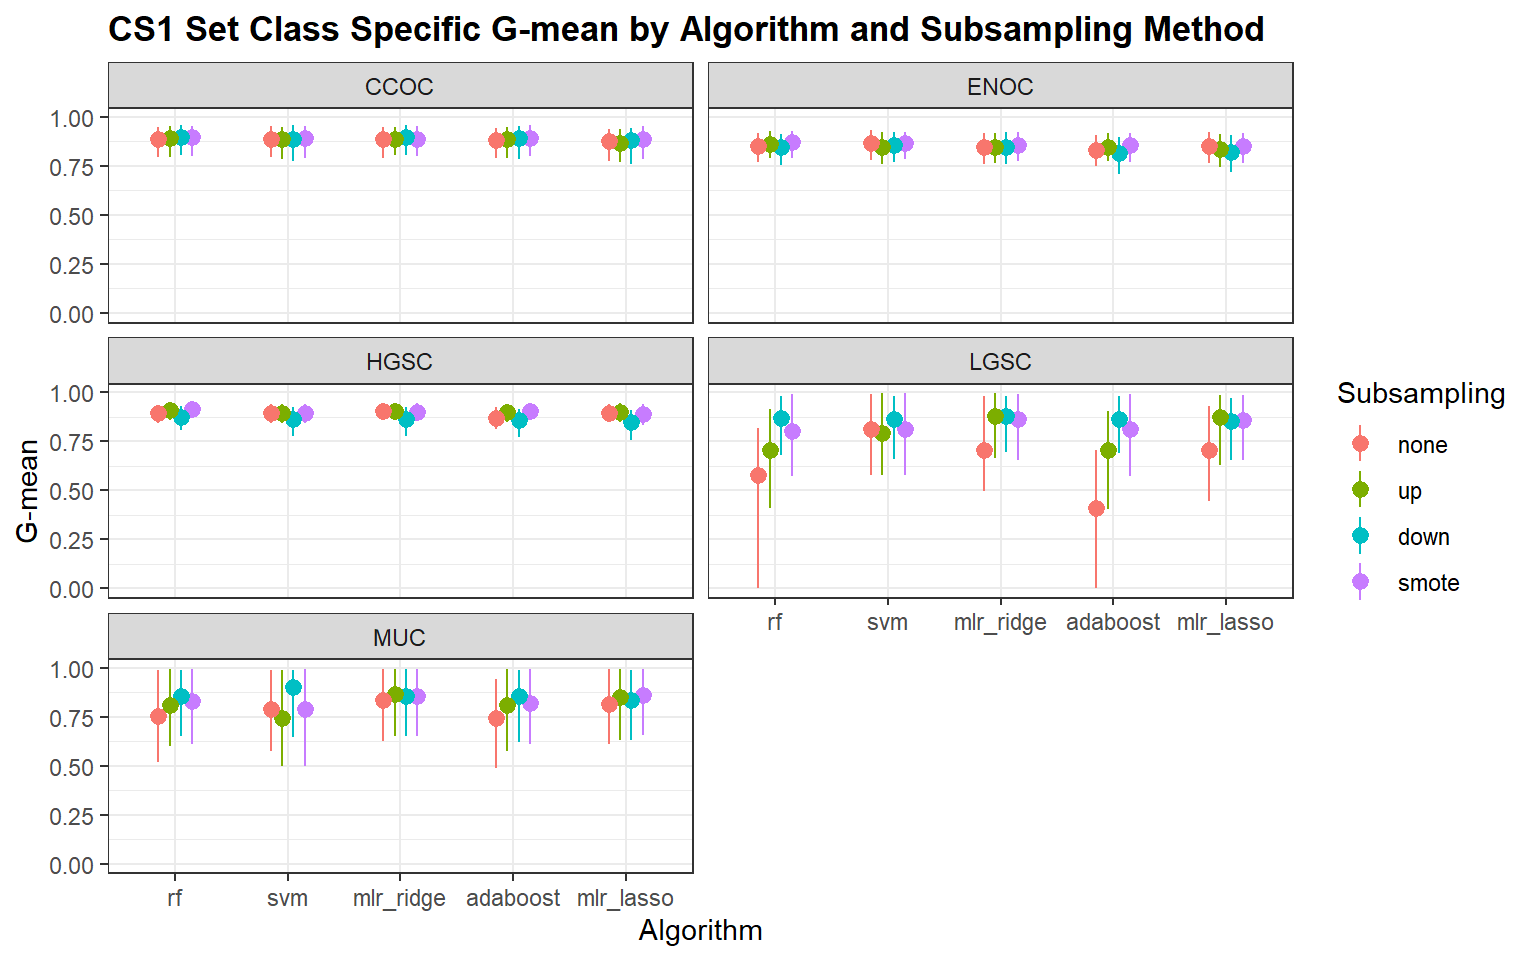
\includegraphics{OV_Histotypes_RSF_files/figure-latex/cs1-gmean-class-1} 

}

\caption{CS1 Set Class-Specific G-mean}\label{fig:cs1-gmean-class}
\end{figure}

\begin{table}

\caption{\label{tab:cs1-gmean-class-table}CS1 Set Class-Specific G-mean by Algorithm and Subsampling Method}
\centering
\begin{tabular}[t]{l|l|l|l|l|l|l}
\hline
sampling & histotype & rf & svm & mlr\_ridge & adaboost & mlr\_lasso\\
\hline
none & CCOC & 0.889 & 0.889 & 0.889 & 0.884 & 0.879\\
\hline
none & ENOC & 0.854 & 0.868 & 0.845 & 0.831 & 0.851\\
\hline
none & HGSC & 0.892 & 0.896 & 0.905 & 0.871 & 0.896\\
\hline
none & LGSC & 0.577 & 0.812 & 0.707 & 0.408 & 0.707\\
\hline
none & MUC & 0.756 & 0.791 & 0.836 & 0.745 & 0.816\\
\hline
up & CCOC & 0.893 & 0.886 & 0.889 & 0.886 & 0.868\\
\hline
up & ENOC & 0.863 & 0.848 & 0.847 & 0.848 & 0.836\\
\hline
up & HGSC & 0.909 & 0.895 & 0.906 & 0.898 & 0.899\\
\hline
up & LGSC & 0.707 & 0.793 & 0.88 & 0.703 & 0.873\\
\hline
up & MUC & 0.812 & 0.745 & 0.866 & 0.808 & 0.853\\
\hline
down & CCOC & 0.896 & 0.889 & 0.897 & 0.89 & 0.883\\
\hline
down & ENOC & 0.847 & 0.859 & 0.848 & 0.817 & 0.823\\
\hline
down & HGSC & 0.873 & 0.866 & 0.862 & 0.861 & 0.848\\
\hline
down & LGSC & 0.871 & 0.865 & 0.877 & 0.866 & 0.851\\
\hline
down & MUC & 0.854 & 0.902 & 0.856 & 0.855 & 0.837\\
\hline
smote & CCOC & 0.895 & 0.892 & 0.889 & 0.893 & 0.887\\
\hline
smote & ENOC & 0.87 & 0.868 & 0.856 & 0.856 & 0.853\\
\hline
smote & HGSC & \textbf{0.913} & 0.897 & 0.902 & 0.904 & 0.89\\
\hline
smote & LGSC & 0.804 & 0.812 & 0.861 & 0.812 & 0.857\\
\hline
smote & MUC & 0.832 & 0.791 & 0.857 & 0.82 & 0.861\\
\hline
\end{tabular}
\end{table}

\hypertarget{cs2-set}{%
\section{CS2 Set}\label{cs2-set}}

\hypertarget{accuracy-3}{%
\subsection{Accuracy}\label{accuracy-3}}

\begin{figure}[H]

{\centering 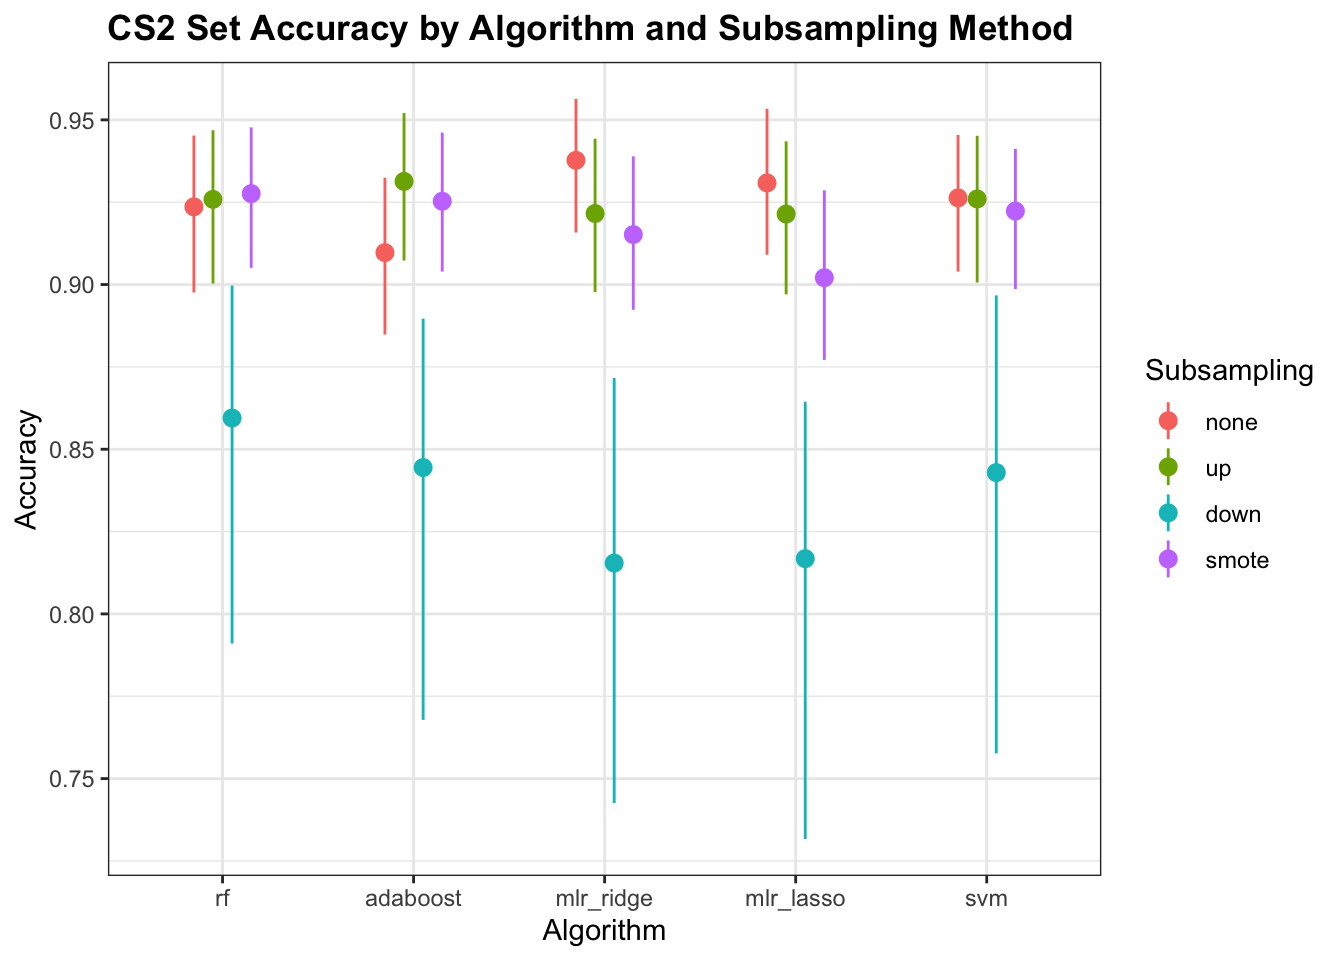
\includegraphics{OV_Histotypes_RSF_files/figure-latex/cs2-accuracy-1} 

}

\caption{CS2 Set Accuracy}\label{fig:cs2-accuracy}
\end{figure}

\begin{table}

\caption{\label{tab:cs2-accuracy-table}CS2 Set Accuracy by Algorithm and Subsampling Method}
\centering
\begin{tabular}[t]{l|l|l|l|l|l}
\hline
sampling & rf & svm & mlr\_ridge & adaboost & mlr\_lasso\\
\hline
none & 0.921 & 0.925 & \textbf{0.933} & 0.905 & 0.927\\
\hline
up & 0.925 & 0.923 & 0.918 & 0.93 & 0.916\\
\hline
down & 0.855 & 0.838 & 0.812 & 0.839 & 0.811\\
\hline
smote & 0.925 & 0.92 & 0.909 & 0.921 & 0.896\\
\hline
\end{tabular}
\end{table}

\begin{figure}[H]

{\centering 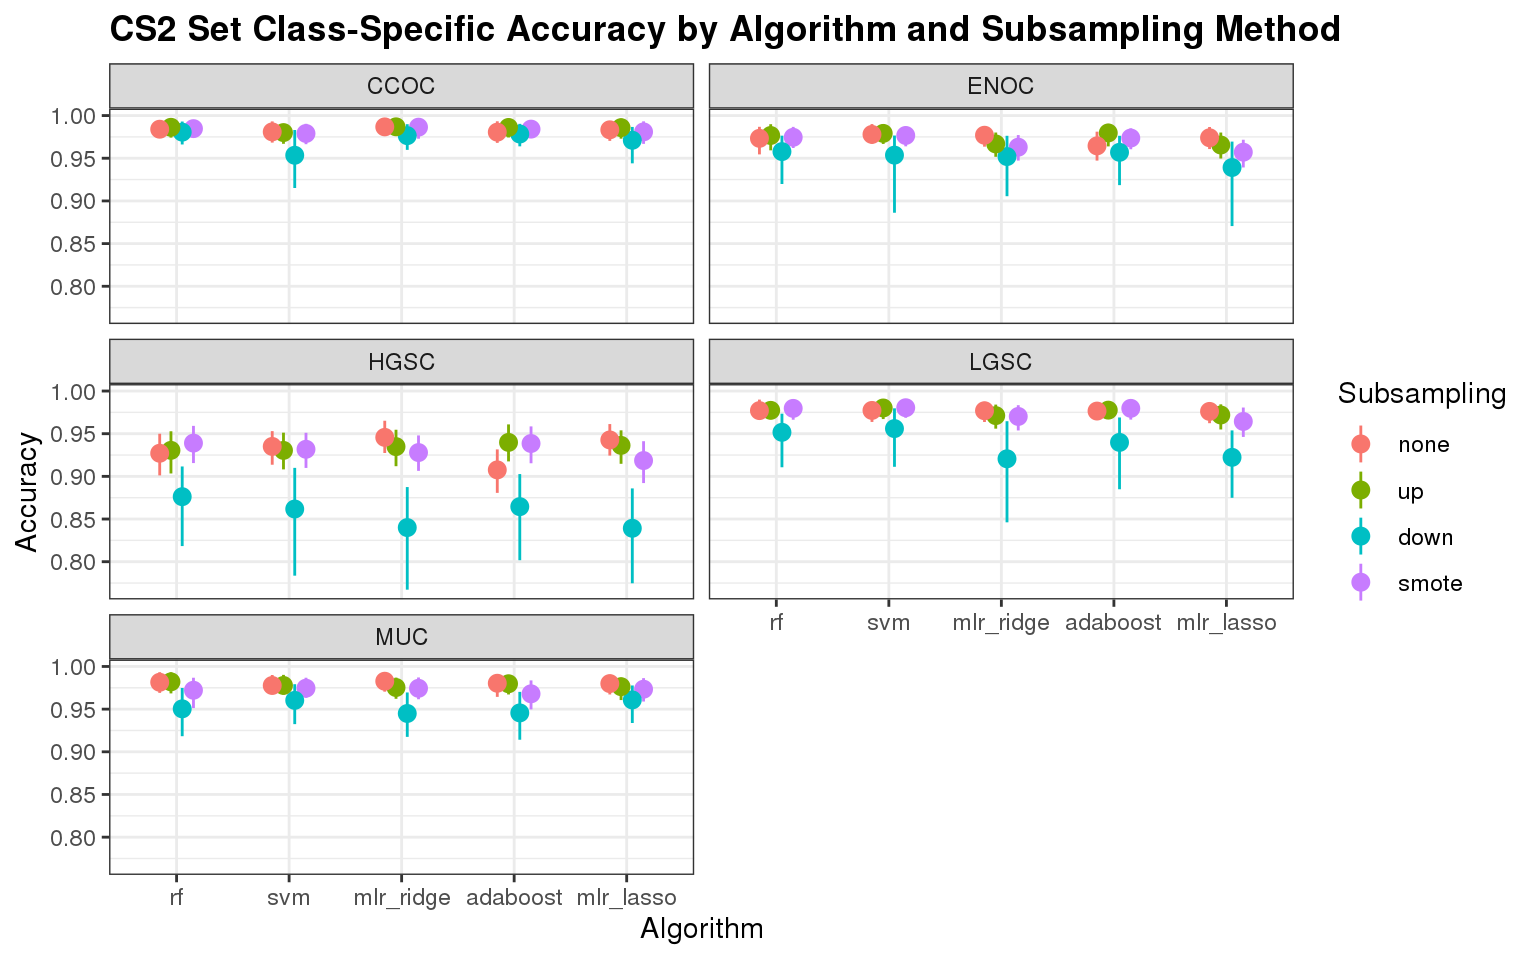
\includegraphics{OV_Histotypes_RSF_files/figure-latex/cs2-accuracy-class-1} 

}

\caption{CS2 Set Class-Specific Accuracy}\label{fig:cs2-accuracy-class}
\end{figure}

\begin{table}

\caption{\label{tab:cs2-accuracy-class-table}CS2 Set Class-Specific Accuracy by Algorithm and Subsampling Method}
\centering
\begin{tabular}[t]{l|l|l|l|l|l|l}
\hline
sampling & histotype & rf & svm & mlr\_ridge & adaboost & mlr\_lasso\\
\hline
none & CCOC & 0.984 & 0.981 & \textbf{0.987} & 0.981 & 0.983\\
\hline
none & ENOC & 0.973 & 0.978 & 0.977 & 0.965 & 0.974\\
\hline
none & HGSC & 0.927 & 0.935 & 0.946 & 0.908 & 0.943\\
\hline
none & LGSC & 0.977 & 0.977 & 0.977 & 0.977 & 0.976\\
\hline
none & MUC & 0.981 & 0.978 & 0.983 & 0.98 & 0.98\\
\hline
up & CCOC & 0.986 & 0.98 & \textbf{0.987} & 0.986 & 0.986\\
\hline
up & ENOC & 0.977 & 0.979 & 0.967 & 0.98 & 0.966\\
\hline
up & HGSC & 0.93 & 0.93 & 0.935 & 0.94 & 0.936\\
\hline
up & LGSC & 0.977 & 0.98 & 0.971 & 0.978 & 0.972\\
\hline
up & MUC & 0.982 & 0.978 & 0.975 & 0.98 & 0.976\\
\hline
down & CCOC & 0.981 & 0.953 & 0.976 & 0.978 & 0.971\\
\hline
down & ENOC & 0.958 & 0.954 & 0.952 & 0.957 & 0.939\\
\hline
down & HGSC & 0.876 & 0.862 & 0.84 & 0.865 & 0.839\\
\hline
down & LGSC & 0.952 & 0.956 & 0.921 & 0.94 & 0.922\\
\hline
down & MUC & 0.95 & 0.96 & 0.945 & 0.946 & 0.961\\
\hline
smote & CCOC & 0.985 & 0.979 & 0.986 & 0.984 & 0.981\\
\hline
smote & ENOC & 0.975 & 0.977 & 0.963 & 0.974 & 0.957\\
\hline
smote & HGSC & 0.939 & 0.932 & 0.928 & 0.939 & 0.919\\
\hline
smote & LGSC & 0.98 & 0.98 & 0.97 & 0.98 & 0.964\\
\hline
smote & MUC & 0.972 & 0.975 & 0.974 & 0.968 & 0.973\\
\hline
\end{tabular}
\end{table}

\hypertarget{f1-score-3}{%
\subsection{F1-Score}\label{f1-score-3}}

\begin{figure}[H]

{\centering 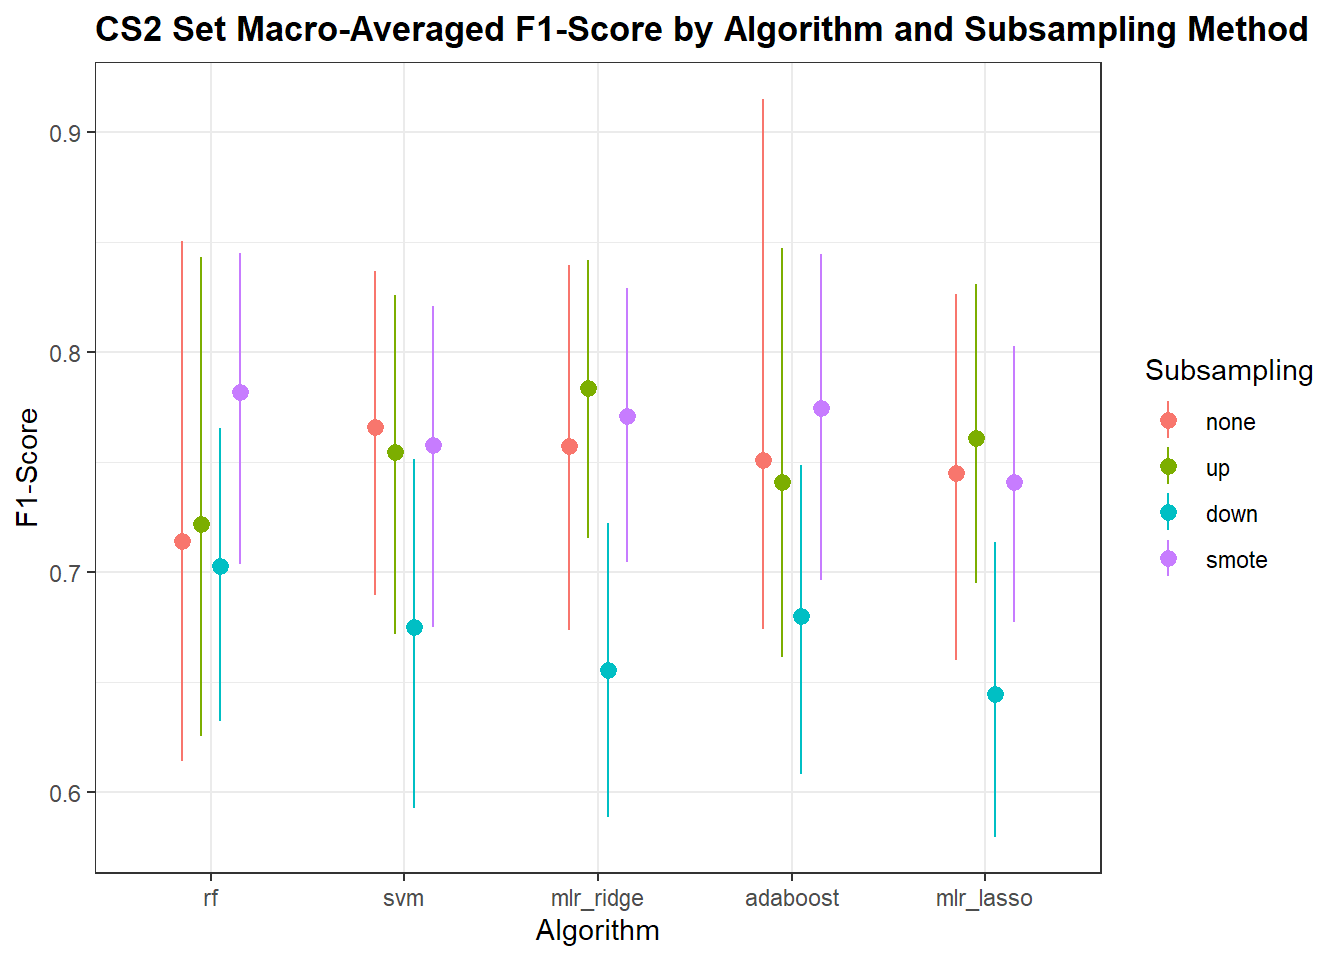
\includegraphics{OV_Histotypes_RSF_files/figure-latex/cs2-f1-1} 

}

\caption{CS2 Set F1-Score}\label{fig:cs2-f1}
\end{figure}

\begin{table}

\caption{\label{tab:cs2-f1-table}CS2 Set Macro-Averaged F1-Score by Algorithm and Subsampling Method}
\centering
\begin{tabular}[t]{l|l|l|l|l|l}
\hline
sampling & rf & svm & mlr\_ridge & adaboost & mlr\_lasso\\
\hline
none & 0.718 & 0.762 & 0.752 & 0.736 & 0.74\\
\hline
up & 0.719 & 0.751 & 0.773 & 0.74 & 0.754\\
\hline
down & 0.699 & 0.668 & 0.652 & 0.675 & 0.645\\
\hline
smote & \textbf{0.782} & 0.755 & 0.762 & 0.769 & 0.732\\
\hline
\end{tabular}
\end{table}

\begin{figure}[H]

{\centering 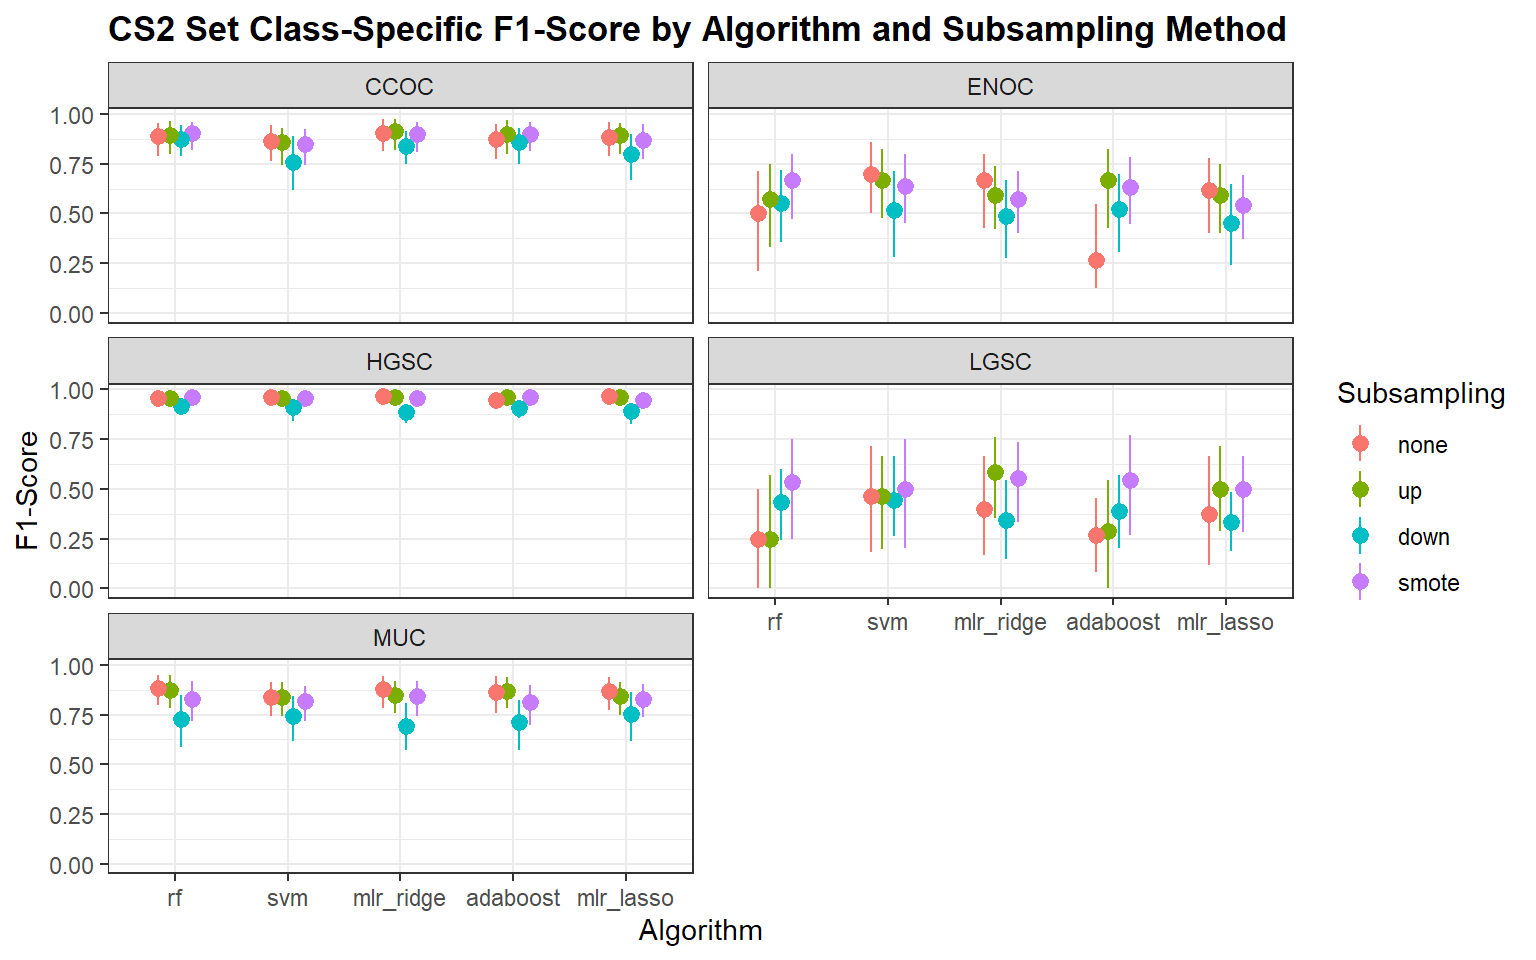
\includegraphics{OV_Histotypes_RSF_files/figure-latex/cs2-f1-class-1} 

}

\caption{CS2 Set Class-Specific F1-Score}\label{fig:cs2-f1-class}
\end{figure}

\begin{table}

\caption{\label{tab:cs2-f1-class-table}CS2 Set Class-Specific F1-Score by Algorithm and Subsampling Method}
\centering
\begin{tabular}[t]{l|l|l|l|l|l|l}
\hline
sampling & histotype & rf & svm & mlr\_ridge & adaboost & mlr\_lasso\\
\hline
none & CCOC & 0.889 & 0.857 & 0.905 & 0.857 & 0.878\\
\hline
none & ENOC & 0.5 & 0.667 & 0.636 & 0.222 & 0.609\\
\hline
none & HGSC & 0.955 & 0.96 & \textbf{0.966} & 0.945 & 0.964\\
\hline
none & LGSC & 0.222 & 0.5 & 0.364 & 0.268 & 0.4\\
\hline
none & MUC & 0.87 & 0.842 & 0.875 & 0.851 & 0.863\\
\hline
up & CCOC & 0.894 & 0.842 & 0.909 & 0.9 & 0.896\\
\hline
up & ENOC & 0.571 & 0.667 & 0.606 & 0.667 & 0.581\\
\hline
up & HGSC & 0.958 & 0.957 & 0.958 & 0.963 & 0.959\\
\hline
up & LGSC & 0.25 & 0.5 & 0.571 & 0.308 & 0.526\\
\hline
up & MUC & 0.864 & 0.833 & 0.84 & 0.86 & 0.837\\
\hline
down & CCOC & 0.875 & 0.739 & 0.84 & 0.863 & 0.809\\
\hline
down & ENOC & 0.563 & 0.519 & 0.515 & 0.545 & 0.452\\
\hline
down & HGSC & 0.916 & 0.907 & 0.888 & 0.908 & 0.89\\
\hline
down & LGSC & 0.435 & 0.444 & 0.341 & 0.375 & 0.34\\
\hline
down & MUC & 0.72 & 0.742 & 0.696 & 0.7 & 0.75\\
\hline
smote & CCOC & 0.9 & 0.839 & 0.903 & 0.898 & 0.872\\
\hline
smote & ENOC & 0.667 & 0.632 & 0.581 & 0.645 & 0.533\\
\hline
smote & HGSC & 0.961 & 0.958 & 0.953 & 0.961 & 0.947\\
\hline
smote & LGSC & 0.556 & 0.545 & 0.545 & 0.556 & 0.5\\
\hline
smote & MUC & 0.821 & 0.818 & 0.833 & 0.8 & 0.824\\
\hline
\end{tabular}
\end{table}

\hypertarget{kappa-3}{%
\subsection{Kappa}\label{kappa-3}}

\begin{figure}[H]

{\centering 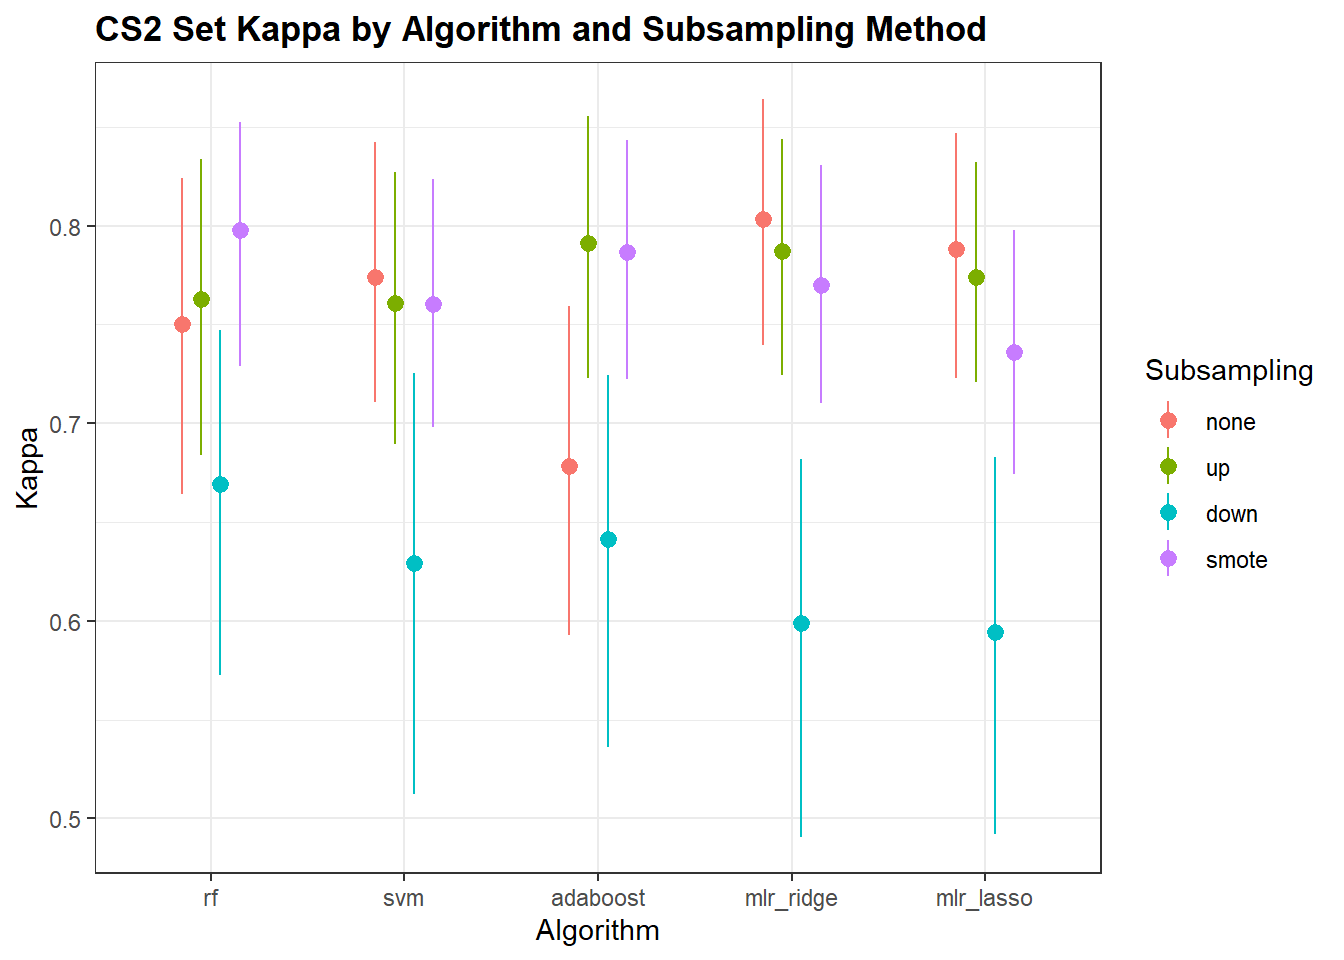
\includegraphics{OV_Histotypes_RSF_files/figure-latex/cs2-kappa-1} 

}

\caption{CS2 Set Kappa}\label{fig:cs2-kappa}
\end{figure}

\begin{table}

\caption{\label{tab:cs2-kappa-table}CS2 Set Kappa by Algorithm and Subsampling Method}
\centering
\begin{tabular}[t]{l|l|l|l|l|l}
\hline
sampling & rf & svm & mlr\_ridge & adaboost & mlr\_lasso\\
\hline
none & 0.75 & 0.774 & \textbf{0.803} & 0.678 & 0.788\\
\hline
up & 0.763 & 0.76 & 0.787 & 0.791 & 0.775\\
\hline
down & 0.67 & 0.629 & 0.601 & 0.642 & 0.594\\
\hline
smote & 0.798 & 0.762 & 0.77 & 0.788 & 0.736\\
\hline
\end{tabular}
\end{table}

\begin{figure}[H]

{\centering 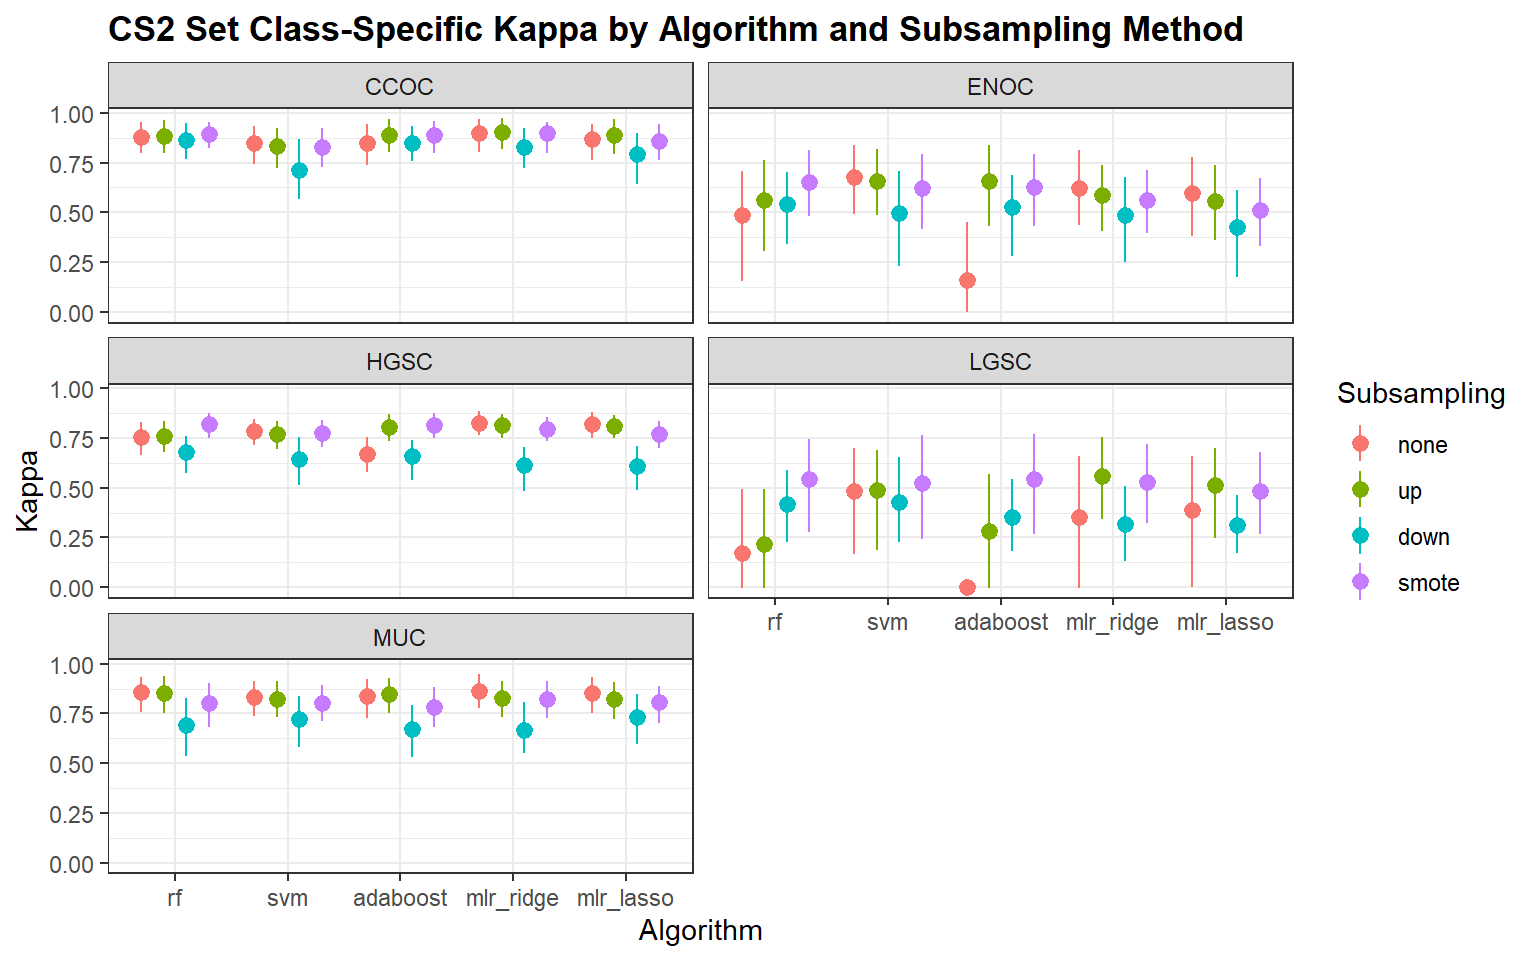
\includegraphics{OV_Histotypes_RSF_files/figure-latex/cs2-kappa-class-1} 

}

\caption{CS2 Set Class-Specific Kappa}\label{fig:cs2-kappa-class}
\end{figure}

\begin{table}

\caption{\label{tab:cs2-kappa-class-table}CS2 Set Class-Specific Kappa by Algorithm and Subsampling Method}
\centering
\begin{tabular}[t]{l|l|l|l|l|l|l}
\hline
sampling & histotype & rf & svm & mlr\_ridge & adaboost & mlr\_lasso\\
\hline
none & CCOC & 0.88 & 0.849 & 0.897 & 0.846 & 0.869\\
\hline
none & ENOC & 0.484 & 0.661 & 0.623 & 0.162 & 0.595\\
\hline
none & HGSC & 0.754 & 0.786 & 0.828 & 0.669 & 0.82\\
\hline
none & LGSC & 0.173 & 0.486 & 0.353 & 0 & 0.386\\
\hline
none & MUC & 0.859 & 0.831 & 0.865 & 0.84 & 0.85\\
\hline
up & CCOC & 0.885 & 0.831 & \textbf{0.902} & 0.893 & 0.888\\
\hline
up & ENOC & 0.559 & 0.656 & 0.588 & 0.655 & 0.559\\
\hline
up & HGSC & 0.761 & 0.769 & 0.813 & 0.804 & 0.812\\
\hline
up & LGSC & 0.214 & 0.488 & 0.558 & 0.282 & 0.512\\
\hline
up & MUC & 0.854 & 0.823 & 0.826 & 0.848 & 0.825\\
\hline
down & CCOC & 0.864 & 0.714 & 0.826 & 0.85 & 0.793\\
\hline
down & ENOC & 0.542 & 0.494 & 0.49 & 0.528 & 0.423\\
\hline
down & HGSC & 0.68 & 0.645 & 0.614 & 0.657 & 0.605\\
\hline
down & LGSC & 0.418 & 0.425 & 0.313 & 0.352 & 0.312\\
\hline
down & MUC & 0.693 & 0.72 & 0.665 & 0.673 & 0.73\\
\hline
smote & CCOC & 0.893 & 0.83 & 0.897 & 0.889 & 0.863\\
\hline
smote & ENOC & 0.655 & 0.62 & 0.559 & 0.627 & 0.511\\
\hline
smote & HGSC & 0.82 & 0.778 & 0.796 & 0.817 & 0.771\\
\hline
smote & LGSC & 0.542 & 0.523 & 0.531 & 0.542 & 0.482\\
\hline
smote & MUC & 0.805 & 0.805 & 0.82 & 0.783 & 0.809\\
\hline
\end{tabular}
\end{table}

\hypertarget{g-mean-3}{%
\subsection{G-mean}\label{g-mean-3}}

\begin{figure}[H]

{\centering 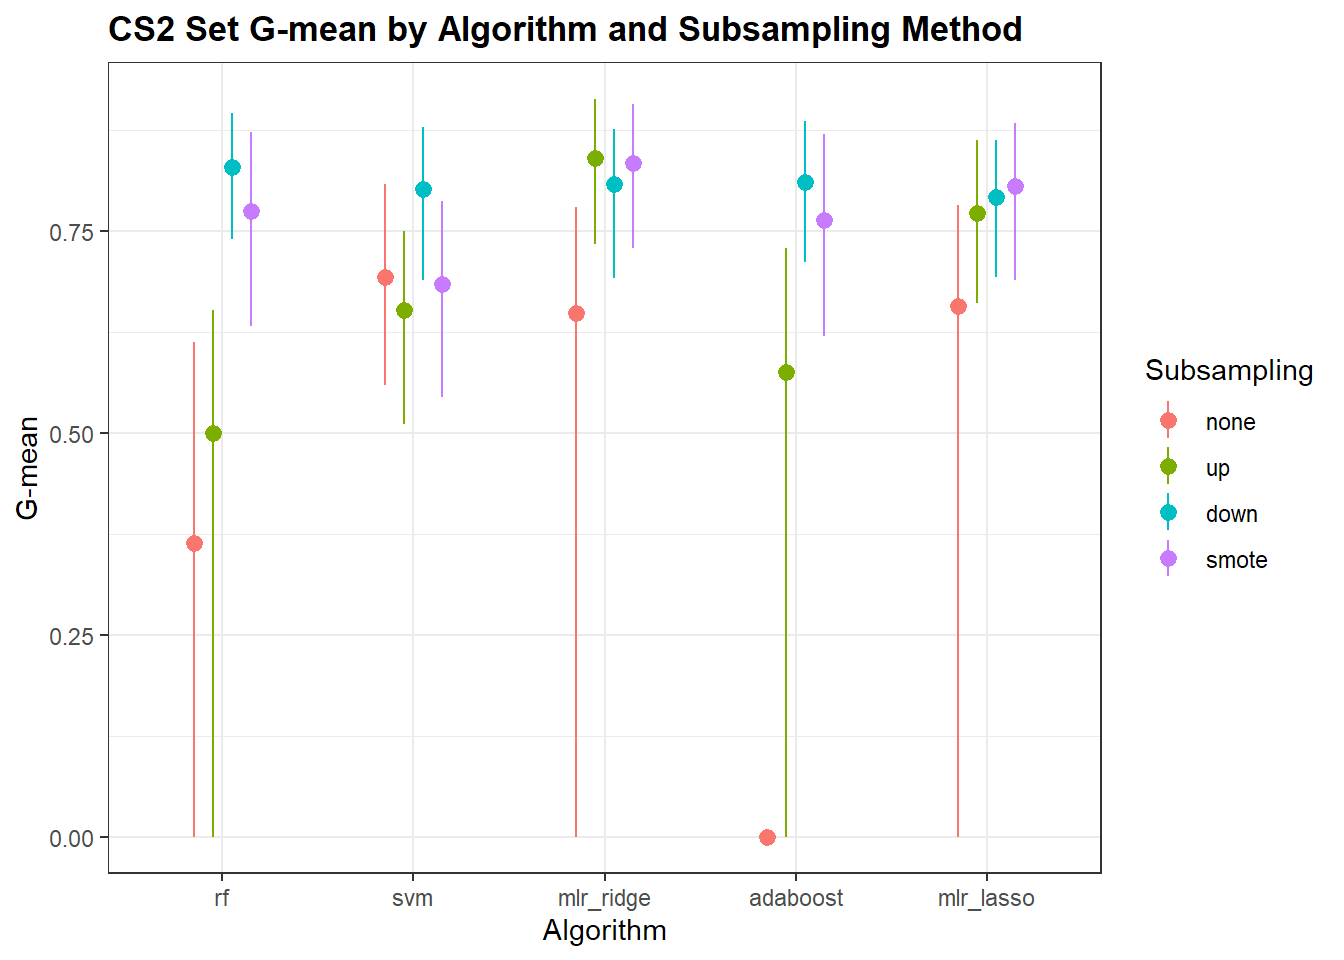
\includegraphics{OV_Histotypes_RSF_files/figure-latex/cs2-gmean-1} 

}

\caption{CS2 Set G-mean}\label{fig:cs2-gmean}
\end{figure}

\begin{table}

\caption{\label{tab:cs2-gmean-table}CS2 Set G-mean by Algorithm and Subsampling Method}
\centering
\begin{tabular}[t]{l|l|l|l|l|l}
\hline
sampling & rf & svm & mlr\_ridge & adaboost & mlr\_lasso\\
\hline
none & 0.401 & 0.683 & 0.645 & 0 & 0.654\\
\hline
up & 0.508 & 0.642 & \textbf{0.835} & 0.589 & 0.766\\
\hline
down & 0.829 & 0.792 & 0.801 & 0.804 & 0.786\\
\hline
smote & 0.776 & 0.677 & 0.825 & 0.763 & 0.801\\
\hline
\end{tabular}
\end{table}

\begin{figure}[H]

{\centering 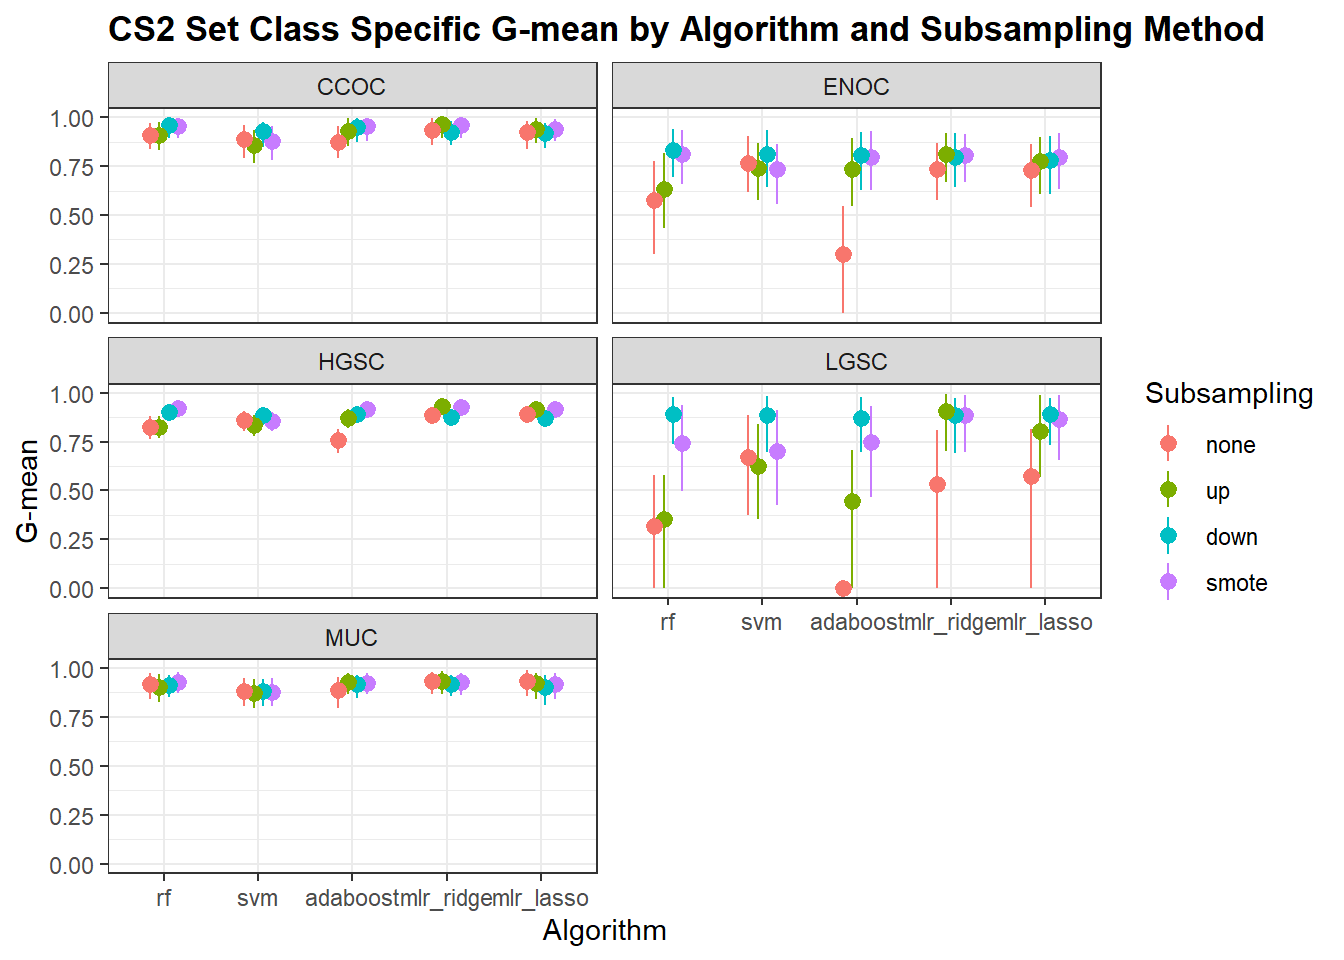
\includegraphics{OV_Histotypes_RSF_files/figure-latex/cs2-gmean-class-1} 

}

\caption{CS2 Set Class-Specific G-mean}\label{fig:cs2-gmean-class}
\end{figure}

\begin{table}

\caption{\label{tab:cs2-gmean-class-table}CS2 Set Class-Specific G-mean by Algorithm and Subsampling Method}
\centering
\begin{tabular}[t]{l|l|l|l|l|l|l}
\hline
sampling & histotype & rf & svm & mlr\_ridge & adaboost & mlr\_lasso\\
\hline
none & CCOC & 0.909 & 0.888 & 0.934 & 0.872 & 0.924\\
\hline
none & ENOC & 0.577 & 0.764 & 0.737 & 0.302 & 0.73\\
\hline
none & HGSC & 0.824 & 0.861 & 0.888 & 0.754 & 0.892\\
\hline
none & LGSC & 0.316 & 0.667 & 0.534 & 0 & 0.575\\
\hline
none & MUC & 0.918 & 0.884 & 0.932 & 0.887 & 0.932\\
\hline
up & CCOC & 0.909 & 0.858 & \textbf{0.965} & 0.929 & 0.941\\
\hline
up & ENOC & 0.632 & 0.737 & 0.81 & 0.73 & 0.78\\
\hline
up & HGSC & 0.826 & 0.836 & 0.933 & 0.871 & 0.919\\
\hline
up & LGSC & 0.354 & 0.628 & 0.902 & 0.446 & 0.807\\
\hline
up & MUC & 0.905 & 0.87 & 0.935 & 0.928 & 0.922\\
\hline
down & CCOC & 0.959 & 0.931 & 0.927 & 0.948 & 0.917\\
\hline
down & ENOC & 0.832 & 0.809 & 0.796 & 0.803 & 0.78\\
\hline
down & HGSC & 0.901 & 0.884 & 0.878 & 0.891 & 0.872\\
\hline
down & LGSC & 0.892 & 0.886 & 0.884 & 0.872 & 0.891\\
\hline
down & MUC & 0.916 & 0.882 & 0.92 & 0.917 & 0.901\\
\hline
smote & CCOC & 0.956 & 0.877 & 0.961 & 0.954 & 0.941\\
\hline
smote & ENOC & 0.812 & 0.734 & 0.808 & 0.796 & 0.793\\
\hline
smote & HGSC & 0.919 & 0.857 & 0.928 & 0.918 & 0.919\\
\hline
smote & LGSC & 0.744 & 0.703 & 0.887 & 0.749 & 0.861\\
\hline
smote & MUC & 0.93 & 0.88 & 0.93 & 0.926 & 0.919\\
\hline
\end{tabular}
\end{table}

\hypertarget{smote-kappa-summary}{%
\section{SMOTE Kappa Summary}\label{smote-kappa-summary}}

\begin{figure}[H]

{\centering 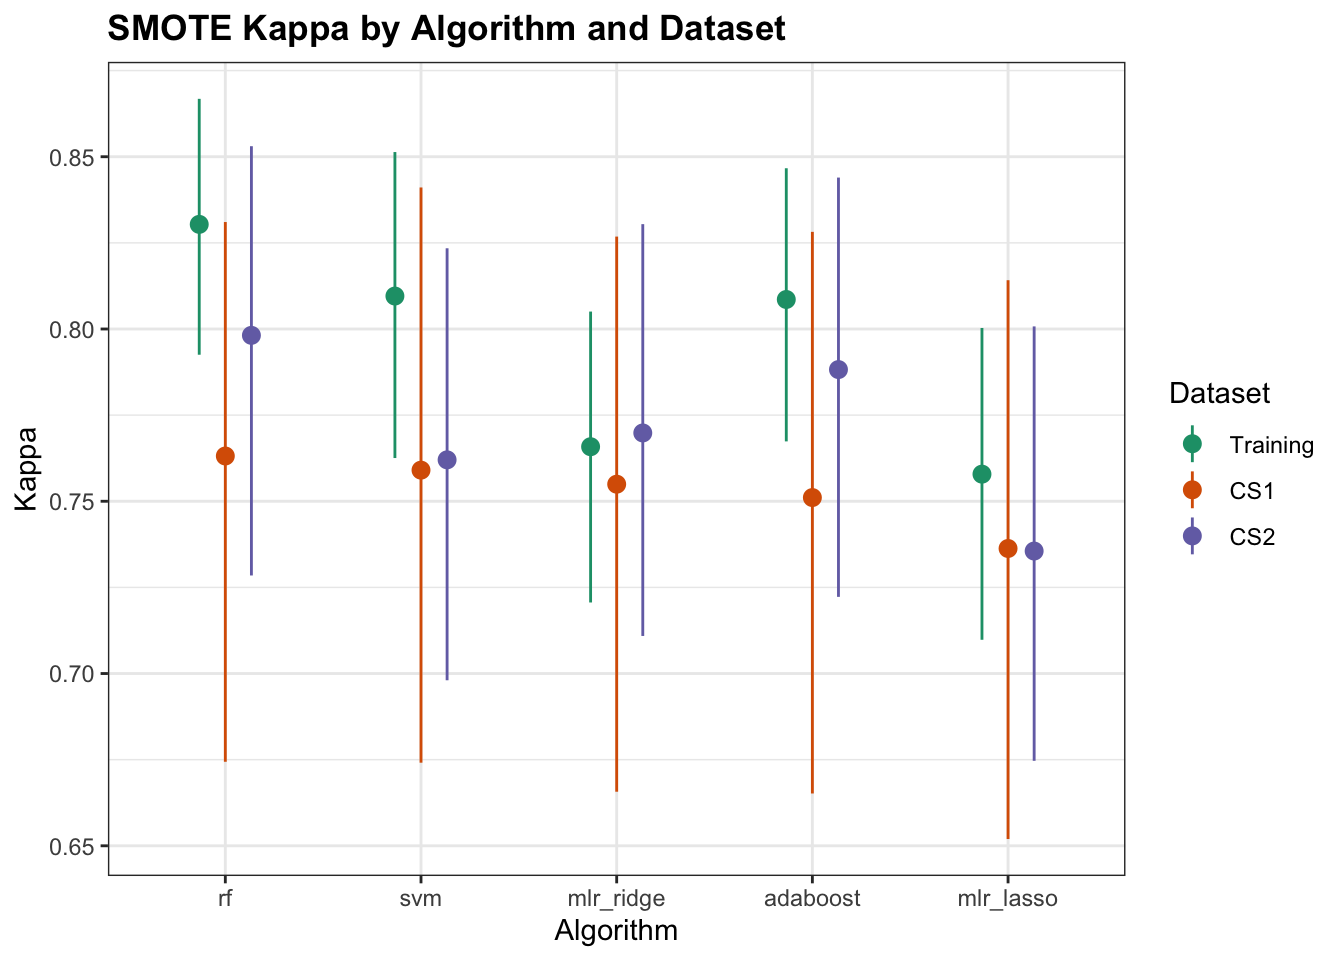
\includegraphics{OV_Histotypes_RSF_files/figure-latex/smote-kappa-1} 

}

\caption{SMOTE Kappa by Algorithm and Dataset}\label{fig:smote-kappa}
\end{figure}

\begin{table}

\caption{\label{tab:smote-kappa-table}SMOTE Kappa by Algorithm and Dataset}
\centering
\begin{tabular}[t]{l|l|l|l|l|l}
\hline
dataset & rf & svm & mlr\_ridge & adaboost & mlr\_lasso\\
\hline
Training & \textbf{0.83} & 0.81 & 0.766 & 0.809 & 0.758\\
\hline
CS1 & 0.763 & 0.759 & 0.755 & 0.751 & 0.736\\
\hline
CS2 & 0.798 & 0.762 & 0.77 & 0.788 & 0.736\\
\hline
\end{tabular}
\end{table}

\begin{figure}[H]

{\centering 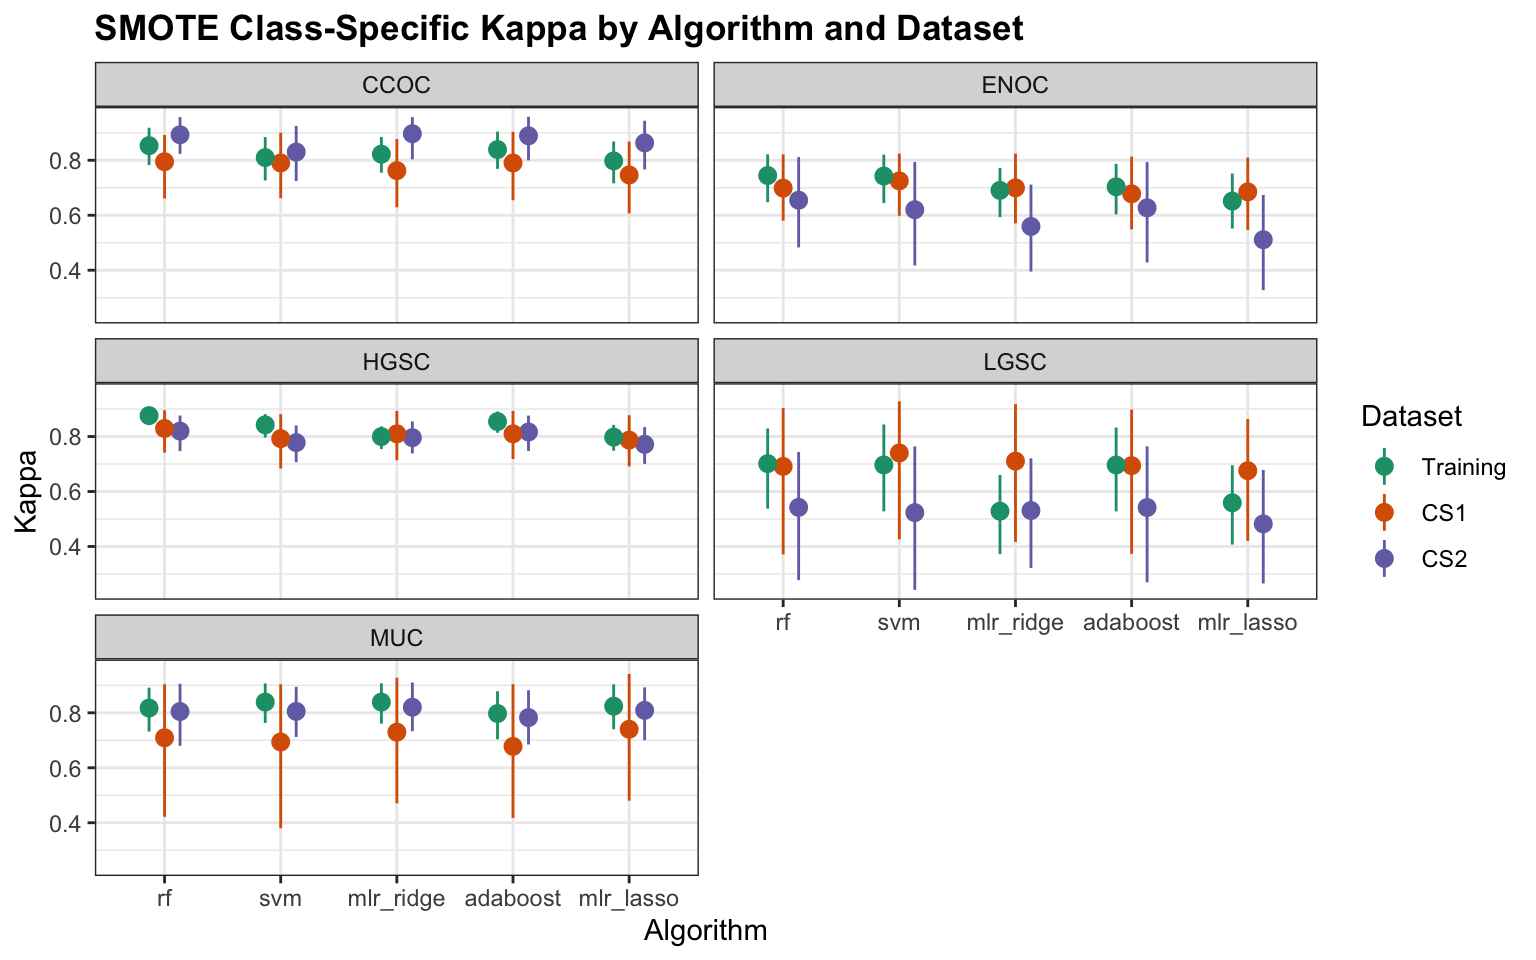
\includegraphics{OV_Histotypes_RSF_files/figure-latex/smote-kappa-class-1} 

}

\caption{SMOTE Class-Specific Kappa by Algorithm and Dataset}\label{fig:smote-kappa-class}
\end{figure}

\hypertarget{overlap-with-spot}{%
\section{Overlap with SPOT}\label{overlap-with-spot}}

There are 13 genes out of the 72 classifier set that overlap with the SPOT signature: HIF1A, CXCL10, DUSP4, SOX17, MITF, CDKN3, BRCA2, CEACAM5, ANXA4, SERPINE1, TCF7L1, CRABP2, DNAJC9.

\hypertarget{rank-aggregation}{%
\section{Rank Aggregation}\label{rank-aggregation}}

\begin{center}\includegraphics{OV_Histotypes_RSF_files/figure-latex/summary-1} \end{center}

The 44 methods (algorithm-sampling combinations) are ordered in the table by their aggregated ranks using the Genetic Algorithm. We see that the best performing methods involve the 2-stage and sequential algorithms.

\hypertarget{test-set-performance}{%
\section{Test Set Performance}\label{test-set-performance}}

Now we'd like to see how our best methods perform in the confirmation and validation sets. The class-specific F1-scores will be used.

The top 4 methods are:

\begin{itemize}
\tightlist
\item
  \textbf{2S-rf-none}: 2-step method using random forest algorithm with no subsampling
\item
  \textbf{sequential-none}: sequential algorithm with no subsampling. The sequence of models and algorithms used are:

  \begin{itemize}
  \tightlist
  \item
    HGSC vs.~non-HGSC using SVM
  \item
    MUC vs.~non-MUC using ridge regression
  \item
    CCOC vs.~non-CCOC using random forest
  \item
    ENOC vs.~LGSC using SVM
  \end{itemize}
\item
  \textbf{2S-rf-smote}: 2-step method using random forest algorithm with SMOTE subsampling
\item
  \textbf{sequential-smote}: sequential algorithm with SMOTE subsampling. The sequence of models and algorithms used are:

  \begin{itemize}
  \tightlist
  \item
    HGSC vs.~non-HGSC using random forest
  \item
    CCOC vs.~non-CCOC using random forest
  \item
    MUC vs.~non-MUC using SVM
  \item
    ENOC vs.~LGSC using random forest
  \end{itemize}
\end{itemize}

As a comparison we also show the F1-scores from the \textbf{rf-none} to see how the best methods improve from it.

\hypertarget{confirmation-set}{%
\subsection{Confirmation Set}\label{confirmation-set}}

\begin{table}

\caption{\label{tab:confirmation-set}Class-specific F1-scores on Confirmation Sets}
\centering
\begin{tabular}[t]{l|r|r|r|r|r}
\hline
method & HGSC & CCOC & ENOC & LGSC & MUC\\
\hline
2S-rf-none & 0.915 & 0.904 & 0.772 & 0.419 & 0.679\\
\hline
sequential-none & 0.905 & 0.917 & 0.917 & 0.485 & 0.711\\
\hline
2S-rf-smote & 0.908 & 0.878 & 0.750 & 0.383 & 0.691\\
\hline
sequential-smote & 0.907 & 0.923 & 0.916 & 0.514 & 0.679\\
\hline
rf-none & 0.893 & 0.887 & 0.486 & 0.133 & 0.745\\
\hline
\end{tabular}
\end{table}

In the confirmation set, \textbf{2S-rf-none} improves drastically in LGSC classification compard to \textbf{rf-none}, with moderate improvement in ENOC, and minor improvement in HGSC and CCOC. There is a decrease in MUC performance. \textbf{sequential-none} improves on \textbf{2S-rf-none} in all classes except for marginal decrease in HGSC performance.

\hypertarget{validation-set}{%
\subsection{Validation Set}\label{validation-set}}

\begin{table}

\caption{\label{tab:validation-set}Class-specific F1-scores on Validation Sets}
\centering
\begin{tabular}[t]{l|r|r|r|r|r}
\hline
method & HGSC & CCOC & ENOC & LGSC & MUC\\
\hline
2S-rf-none & 0.931 & 0.920 & 0.823 & 0.750 & 0.571\\
\hline
sequential-none & 0.943 & 0.862 & 0.964 & 0.750 & 0.725\\
\hline
2S-rf-smote & 0.917 & 0.920 & 0.788 & 0.732 & 0.538\\
\hline
sequential-smote & 0.926 & 0.902 & 0.953 & 0.698 & 0.617\\
\hline
rf-none & 0.920 & 0.839 & 0.540 & 0.174 & 0.686\\
\hline
\end{tabular}
\end{table}

Similarly in the validation set, \textbf{2S-rf-none} improves drastically in LGSC classification compared to \textbf{rf-none}, with large improvement in ENOC, and minor improvement in HGSC and CCOC. There is a decrease in MUC performance. \textbf{sequential-none} improves on \textbf{2S-rf-none} in all classes except for a small decrease in CCOC performance and same performance for LGSC.

  \bibliography{packages.bib}
\addcontentsline{toc}{chapter}{\bibname}

\end{document}
